\chapter{The sensitivity of CLIC to anomalous gauge couplings through vector boson scattering}
\label{chap:PhysicsAnalysis}

\chapterquote{Kids, you tried your best, and you failed miserably.  The lesson is, never try.}%
{Homer Simpson}

%========================================================================================
%========================================================================================

\section{Motivation}
Vector boson scattering is the interaction of the form $\text{VV} \rightarrow \text{VV}$ where V is any of the electroweak gauge bosons $\text{W}^{+}$, $\text{W}^{-}$, Z or $\gamma$.  This is an interesting process to look at because it gives a detailed understanding of how the standard model Higgs is able to unitarise the otherwise unbounded cross section for longitudinal gauge boson scattering.  Vector boson scattering also provides insights into beyond standard model physics that impacts the electroweak sector through the probing of anomalous triple and quartic gauge couplings.  Presented in this section is an analysis into the sensitivity of CLIC to two of these anomalous quartic gauge couplings through the vector boson scattering process.

Triple and quartic gauge couplings lead to interactions of the form $\text{V} \rightarrow \text{VV}$ and $\text{VV} \rightarrow \text{VV}$ respectively.  In the standard model there are five permissible  vertices, shown in figure \ref{fig:smtripleandquarticvertices}, which arise from the kinematic term $\mathcal{L}_{kin} = -\frac{1}{4}B_{\mu\nu}B^{\mu\nu} - \frac{1}{4}W_{\mu\nu}W^{\mu\nu}$.
% Feynam diagrams of triple and quartic vertices in the standard model.
\begin{figure}[h!]
\subfloat[]{\label{fig:smvertex1}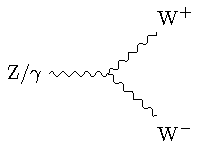
\includegraphics[width=0.3\textwidth]{PhysicsAnalysis/Plots/FeynmanDiagrams/SMVertex1.pdf}} 
\subfloat[]{\label{fig:smvertex2}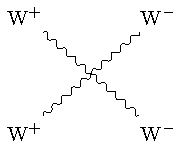
\includegraphics[width=0.3\textwidth]{PhysicsAnalysis/Plots/FeynmanDiagrams/SMVertex2.pdf}} 
\subfloat[]{\label{fig:smvertex3}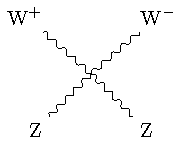
\includegraphics[width=0.3\textwidth]{PhysicsAnalysis/Plots/FeynmanDiagrams/SMVertex3.pdf}} \hfill
\subfloat[]{\label{fig:smvertex4}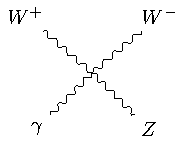
\includegraphics[width=0.3\textwidth]{PhysicsAnalysis/Plots/FeynmanDiagrams/SMVertex4.pdf}} 
\subfloat[]{\label{fig:smvertex5}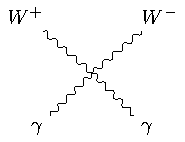
\includegraphics[width=0.3\textwidth]{PhysicsAnalysis/Plots/FeynmanDiagrams/SMVertex5.pdf}} 
\caption[Gauge boson self-coupling vertices in the standard model.]{Gauge boson self-coupling vertices in the standard model.}
\label{fig:smtripleandquarticvertices}
\end{figure}

Anomalous triple and quartic gauge couplings are introduced as parameters in effective field theories (EFTs).  These couplings either modify the standard model triple and quartic gauge boson couplings or introduce new triple and quartic couplings that were previously forbidden.  EFTs are a mathematical construct designed to introduce new physics in a manor that builds upon the standard model.  They work under the assumption than new physics exists at an energy scale, $\Lambda$, that is much higher than the energy scales currently accessible to modern day particle physics experiments.  In limit $\Lambda \rightarrow \infty$ the standard model should be reproduced as the new physics becomes kinematically inaccessible.  Such theories are model independent, giving them a wide span in the search for new physics.  A classic example of an EFT theory is the Fermi theory for beta decay \cite{Fermi:1934hr}.  The weak interaction occurring when a neutron decays into a proton, electron and anti-neutrino can, at energies much below the mass of the W boson, be treated as a four-point vertex with quartic coupling strength $\text{G}_{F}$, the Fermi Coupling constant as shown in figure \ref{fig:fermitheory}.

\begin{figure}[h!]
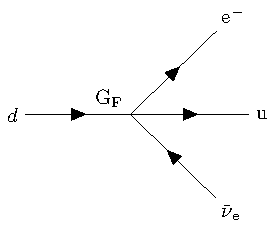
\includegraphics[width=0.5\textwidth]{PhysicsAnalysis/Plots/FeynmanDiagrams/FermiTheory.pdf}
\caption[Four-point vertex proposed for explanation of beta decay by Fermi.]{Four-point vertex proposed for explanation of beta decay by Fermi.} 
\label{fig:fermitheory}
\end{figure}

This analysis examines the anomalous quartic gauge couplings $\alpha_{4}$ and $\alpha_{5}$, which are introduced as part of an EFT described in chapter \ref{chap:anomalousgaugecouplingtheory}.  They appear in the Lagrangian through the following terms 

\begin{equation}
\alpha_{4}[\text{Tr}(V^{\mu}V_{\mu})]^{2} \text{ and } \alpha_{5}\text{Tr}(V^{\mu}V_{\nu})] \text{Tr}(V^{\nu}V_{\mu})]\text{,}
\end{equation}

\noindent where $V_{\mu}$ corresponds, in a carefully chosen gauge, to a linear combination of the massive gauge bosons $\text{W}^{+}$, $\text{W}^{-}$ and Z.  These terms affect the coupling constants for the standard model vertices $\text{W}^{+}\text{W}^{-} \rightarrow \text{W}^{+}\text{W}^{-}$ and $\text{W}^{+}\text{W}^{-} \rightarrow \text{Z}\text{Z}$ as well as introducing the new vertex $\text{Z}\text{Z} \rightarrow \text{Z}\text{Z}$.  Vector boson scattering is an appropriate process to consider for a study of the anomalous gauge couplings $\alpha_{4}$ and $\alpha_{5}$ as quartic gauge boson self-interaction vertices will be present in the dominant channels for such interactions.  Example vector boson scattering Feynman diagrams showing sensitivity to quartic gauge boson self-interaction vertices are shown in figure \ref{fig:vectorbosonscatteringclic}. 
% Feynam diagrams of sensitive processes 
\begin{figure}[h!]
\subfloat[]{\label{fig:vbsclic1}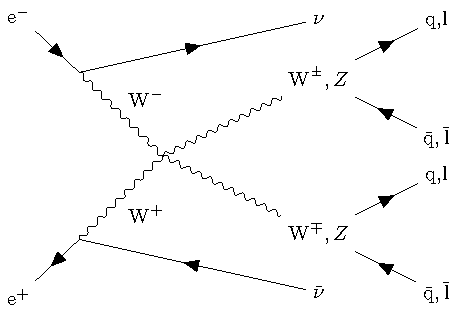
\includegraphics[width=0.5\textwidth]{PhysicsAnalysis/Plots/FeynmanDiagrams/VBSCLIC1.pdf}} \hfill
\subfloat[]{\label{fig:vbsclic2}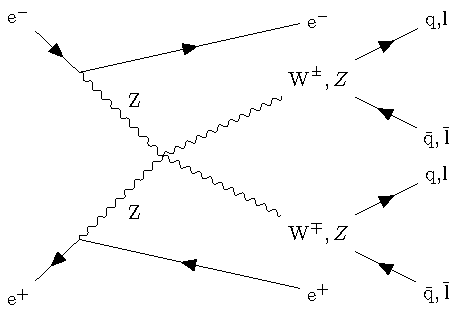
\includegraphics[width=0.5\textwidth]{PhysicsAnalysis/Plots/FeynmanDiagrams/VBSCLIC2.pdf}} \hfill
\subfloat[]{\label{fig:vbsclic3}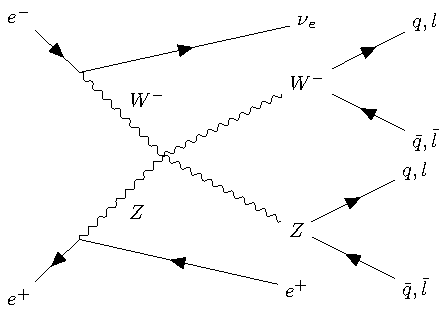
\includegraphics[width=0.5\textwidth]{PhysicsAnalysis/Plots/FeynmanDiagrams/VBSCLIC3.pdf}} \hfill
\subfloat[]{\label{fig:vbsclic4}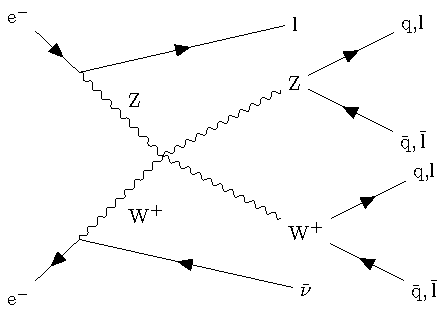
\includegraphics[width=0.5\textwidth]{PhysicsAnalysis/Plots/FeynmanDiagrams/VBSCLIC4.pdf}} \hfill
\caption[Example of vector boson scattering Feynman diagrams showing sensitivity to quartic gauge boson self-interaction vertices.  The diagrams selected here are relevant for the CLIC experiment.  In these diagrams q represents u, $\bar{\text{u}}$, d, $\bar{\text{d}}$, s, $\bar{\text{s}}$, c, $\bar{\text{c}}$, b or $\bar{\text{b}}$;  l represents $\text{e}^{\pm}$, $\mu^{\pm}$ or $\tau^{\pm}$; and $\nu$ represents $\nu_{e}$, $\overline{\nu_{e}}$, $\nu_{\mu}$, $\overline{\nu_{\mu}}$, $\nu_{\tau}$ and $\overline{\nu_{\tau}}$.]{Example of vector boson scattering Feynman diagrams showing sensitivity to quartic gauge boson self-interaction vertices.  The diagrams selected here are relevant for the CLIC experiment.  In these diagrams q represents u, $\bar{\text{u}}$, d, $\bar{\text{d}}$, s, $\bar{\text{s}}$, c, $\bar{\text{c}}$, b or $\bar{\text{b}}$;  l represents $\text{e}^{\pm}$, $\mu^{\pm}$ or $\tau^{\pm}$; and $\nu$ represents $\nu_{e}$, $\overline{\nu_{e}}$, $\nu_{\mu}$, $\overline{\nu_{\mu}}$, $\nu_{\tau}$ and $\overline{\nu_{\tau}}$.}
\label{fig:vectorbosonscatteringclic}
\end{figure}

As CLIC is purposefully deigned for high precision measurements it is ideal for a study into vector boson scattering.  The application of Particle Flow Calorimetry with fine granularity calorimeters gives CLIC excellent jet energy resolution, which allows it to clearly characterise multi-jet final states.  When considering the invariant mass of these paired up jets, the nominal jet energy resolution for CLIC allows for accurate separation of W and Z bosons, which will be invaluable for event selection.  This precision also helps CLIC to characterise final states containing missing energy in the form of neutrinos.  The cross sections for vector boson scattering processes are sufficiently large at the proposed running energies for CLIC to give a large signal sample size for this analysis.  Finally, this study offers the potential to give results several orders of magnitude better than the complementary studies performed at the LHC.  This is due to the reduction in hadronic backgrounds and the larger $\sqrt{s}$ obtained when colliding leptons as opposed to protons.  All of the above reasons make a strong case for performing this analysis at CLIC.  

This study focuses on determining the sensitivity of CLIC to the anomalous gauge couplings based solely upon the vector boson scattering processes where the outgoing bosons decay purely hadronically.  This decision was made as the hadronic channels are the dominant decay modes of the W and the Z boson, with branching fractions of the order of 70\% for both \cite{Beringer:1900zz}, and given CLIC has excellent jet energy resolution.  Therefore, the signal final states in this analysis are: $\nu\nu\text{qqqq}$, $\text{l}\nu\text{qqqq}$ and llqqqq.  

%========================================================================================
%========================================================================================

\section{Event Generation, Simulation and Reconstruction}
\label{sec:eventgenerationandbackgrounds}
Events were generated for this analysis using the Whizard \cite{0708.4233, hep-ph/0102195} version 1.95.  Due to the presence of beamstrahlung photons in the CLIC beam events were generated from collisions of $\text{e}^{+}\text{e}^{-}$, $\text{e}^{+}\gamma$, $\gamma\text{e}^{-}$ and $\gamma\gamma$.  The energy spectra used for all particles involved in these collisions took into account the effects of radiation in the form of beamstrahlung photons and the intrinsic energy spread of the CLIC beam.  Furthermore, events involving the interaction between the electromagnetic field of the beam particles involving quasi-real photon mediators with low momenta, described by the Weizsacker-Williams approximation or the Equivalent Photon Approximation (EPA), were generated using Whizard and included in this analysis.  Fragmentation and hadronisation was implemented using PYTHIA 6.4 \cite{Sjostrand:2006za} that was tuned for OPAL $\text{e}^{+}\text{e}^{-}$ collision data recorded at LEP \cite{Linssen:2012hp}.  The decays of tau leptons was simulated using Tauola \cite{Was:2000st}.  The full list of events simulated for this analysis, along with their standard model cross section at 1.4~TeV can be found in table \ref{table:crosssection1400GeV}.  The samples generated comprise all final states that would be relevant, either as signal or background processes, for an analysis involving the purely hadronic decay channels involved in a vector boson scattering process.  In full they are:

\begin{itemize}
\item Vector boson scattering signal final states that are expected to show sensitivity to the anomalous couplings: $\text{e}^{+}\text{e}^{-} \rightarrow \nu\nu\text{qqqq}$, $\text{e}^{+}\text{e}^{-} \rightarrow \text{l}\nu\text{qqqq}$ and $\text{e}^{+}\text{e}^{-} \rightarrow \text{llqqqq}$
\item Four jet final states arising from $\text{e}^{+}\text{e}^{-}$ interactions: $\text{e}^{+}\text{e}^{-} \rightarrow \text{qqqq}$.
\item Two jet final states arising from $\text{e}^{+}\text{e}^{-}$ interactions: $\text{e}^{+}\text{e}^{-} \rightarrow \nu{\nu}\text{qq}$, $\text{e}^{+}\text{e}^{-} \rightarrow \text{l}\nu\text{qq}$, $\text{e}^{+}\text{e}^{-} \rightarrow \text{llqq}$ and $\text{e}^{+}\text{e}^{-} \rightarrow \text{qq}$.
\item Four jet final states arising from the interactions of either $\text{e}^{+}$ or $\text{e}^{-}$ with a beamstrahlung photon: $\gamma_{\text{BS}}\text{e}^{-} \rightarrow \text{qqqq}\text{e}^{-}$, $\text{e}^{+}\gamma_{\text{BS}} \rightarrow \text{qqqq}\text{e}^{+}$, $\gamma_{\text{BS}}\text{e}^{-} \rightarrow \text{qqqq}\nu$ and $\text{e}^{+}\gamma_{\text{BS}} \rightarrow \text{qqqq}\nu$.
\item Four jet final states arising from the interactions of either $\text{e}^{+}$ or $\text{e}^{-}$ with the electromagnetic field of the opposing beam particle.  These cross sections are calculated using the EPA approximation, which represents the electromagnetic field of the opposing beam particle as a series of photons, so the final states appear as interactions of $\text{e}^{+}$ or $\text{e}^{-}$ with photons: $\gamma_{\text{EPA}}\text{e}^{-} \rightarrow \text{qqqq}\text{e}^{-}$, $\text{e}^{+}\gamma_{\text{EPA}} \rightarrow \text{qqqq}\text{e}^{+}$, $\gamma_{\text{EPA}}\text{e}^{-} \rightarrow \text{qqqq}\nu$ and $\text{e}^{+}\gamma_{\text{EPA}} \rightarrow \text{qqqq}\nu$.
\item Four jet final states arising from the interaction of the electromagnetic fields of opposing beam particles using the EPA approximation: $\gamma_{\text{EPA}}\gamma_{\text{EPA}} \rightarrow \text{qqqq}$.
\item Four jet final states arising from the interaction of the electromagnetic field of either $\text{e}^{+}$ or $\text{e}^{-}$ using the EPA approximation with a beamstrahlung photon: $\gamma_{\text{EPA}}\gamma_{\text{BS}} \rightarrow \text{qqqq}$ or $\gamma_{\text{BS}}\gamma_{\text{EPA}} \rightarrow \text{qqqq}$.
\item Four jet final states arising from the interaction of two beamstrahlung photons: $\gamma_{\text{BS}}\gamma_{\text{BS}} \rightarrow \text{qqqq}$.
\end{itemize}

\noindent In the above list q represents u, $\bar{\text{u}}$, d, $\bar{\text{d}}$, s, $\bar{\text{s}}$, c, $\bar{\text{c}}$, b or $\bar{\text{b}}$;  l represents $\text{e}^{\pm}$, $\mu^{\pm}$ or $\tau^{\pm}$; and $\nu$ represents $\nu_{e}$, $\overline{\nu_{e}}$, $\nu_{\mu}$, $\overline{\nu_{\mu}}$, $\nu_{\tau}$ and $\overline{\nu_{\tau}}$.

\begin{table}[h!]
\centering
\begin{tabular}{ l r }
\hline
Final State & Cross Section 1.4~TeV [fb] \\ 
\hline
$\text{e}^{+}\text{e}^{-} \rightarrow \nu{\nu}\text{qqqq}$ & 24.7 \\
$\text{e}^{+}\text{e}^{-} \rightarrow \text{l}\nu\text{qqqq}$ & 110.4\\
$\text{e}^{+}\text{e}^{-} \rightarrow \text{llqqqq}$ & 62.1\\
$\text{e}^{+}\text{e}^{-} \rightarrow \text{qqqq}$ & 1245.1\\
$\text{e}^{+}\text{e}^{-} \rightarrow \nu{\nu}\text{qq}$ & 787.7\\
$\text{e}^{+}\text{e}^{-} \rightarrow \text{l}\nu\text{qq}$ & 4309.7\\
$\text{e}^{+}\text{e}^{-} \rightarrow \text{llqq}$ & 2725.8\\
$\text{e}^{+}\text{e}^{-} \rightarrow \text{qq}$ & 4009.5\\
$\gamma_{\text{EPA}}\text{e}^{-} \rightarrow \text{qqqq}\text{e}^{-}$ & 287.1\\
$\gamma_{\text{BS}}\text{e}^{-} \rightarrow \text{qqqq}\text{e}^{-}$ & 1160.7\\
$\text{e}^{+}\gamma_{\text{EPA}} \rightarrow \text{qqqq}\text{e}^{+}$ & 286.9\\
$\text{e}^{+}\gamma_{\text{BS}} \rightarrow \text{qqqq}\text{e}^{+}$ & 1156.3\\
$\gamma_{\text{EPA}}\text{e}^{-} \rightarrow \text{qqqq}\nu$ & 32.6\\
$\gamma_{\text{BS}}\text{e}^{-} \rightarrow \text{qqqq}\nu$ & 136.9\\
$\text{e}^{+}\gamma_{\text{EPA}} \rightarrow \text{qqqq}\nu$ & 32.6\\
$\text{e}^{+}\gamma_{\text{BS}} \rightarrow \text{qqqq}\nu$ & 136.4\\
$\gamma_{\text{EPA}}\gamma_{\text{EPA}} \rightarrow \text{qqqq}$ & 753.0\\
$\gamma_{\text{EPA}}\gamma_{\text{BS}} \rightarrow \text{qqqq}$ & 4034.8\\
$\gamma_{\text{BS}}\gamma_{\text{EPA}} \rightarrow \text{qqqq}$ & 4018.7\\
$\gamma_{\text{BS}}\gamma_{\text{BS}} \rightarrow \text{qqqq}$ & 21406.2\\
\hline
\end{tabular}
\caption[Cross sections of signal and background processes at 1.4~TeV]{Cross sections of signal and background processes at 1.4~TeV.  In the above table q represents u, $\bar{\text{u}}$, d, $\bar{\text{d}}$, s, $\bar{\text{s}}$, c, $\bar{\text{c}}$, b or $\bar{\text{b}}$;  l represents $\text{e}^{\pm}$, $\mu^{\pm}$ or $\tau^{\pm}$; and $\nu$ represents $\nu_{e}$, $\overline{\nu_{e}}$, $\nu_{\mu}$, $\overline{\nu_{\mu}}$, $\nu_{\tau}$ and $\overline{\nu_{\tau}}$.  The EPA and BS subscript on the incoming photon indicates whether the photon is generated from the equivalent photon approximation or beamstrahlung.}
\label{table:crosssection1400GeV}
\end{table}

The samples used in this analysis were simulated with the CLID\_ILD detector model \cite{arXiv:1006.3396}.  Further details of this detector model can be found in chapter \ref{chap:reconstructionchain}.  The simulation was performed in MOKKA \cite{MoradeFreitas:2002kj}, a GEANT4 \cite{Agostinelli:2002hh} wrapper providing detailed geometric descriptions of detector concepts for the linear collider.  Events were reconstructed using MARLIN \cite{Gaede:2006pj}, a c++ framework designed for reconstruction at the linear collider.  PandoraPFA \cite{arXiv:0907.3577, arXiv:1209.4039} was used to apply Particle Flow Calorimetry in the reconstruction, the full details of which can be found in chapter \ref{chap:reconstructionchain}.
 
%========================================================================================
%========================================================================================

\section{Modelling of Anomalous Gauge Couplings}
\label{sec:modellingofanomalouscouplings}
It was necessary when generating samples that are sensitive to the anomalous gauge couplings $\alpha_{4}$ and $\alpha_{5}$ to use Whizard version 1.97, instead of the previously quoted version 1.95.  This change was required as version 1.97 contained a unitarisation scheme that ensured cross sections for processes involving longitudinal gauge boson scattering were bound at the energies considered i.e. the TeV scale.  

The sensitivity of an individual event to the anomalous gauge couplings is determined through an event weight. This weight is given by the ratio of the squares of the matrix element used in the cross section calculation, one matrix element using non-zero values of $\alpha_{4}$ and $\alpha_{5}$ and the other matrix element using the standard model values of $\alpha_{4}$ and $\alpha_{5}$, i.e. 0.  The weight varies as a function of $\alpha_{4}$ and $\alpha_{5}$ as well as varying on an event by event basis as the kinematics of the final state changes.  Examples of the event weights as a function of $\alpha_{4}$ and $\alpha_{5}$ for selected events is shown in figure \ref{fig:eventweights1400raw} for 1.4~TeV \nu{\nu}qqqq final state events.

\begin{figure}[h!]
\centering
\subfloat[]{\label{fig:weight1}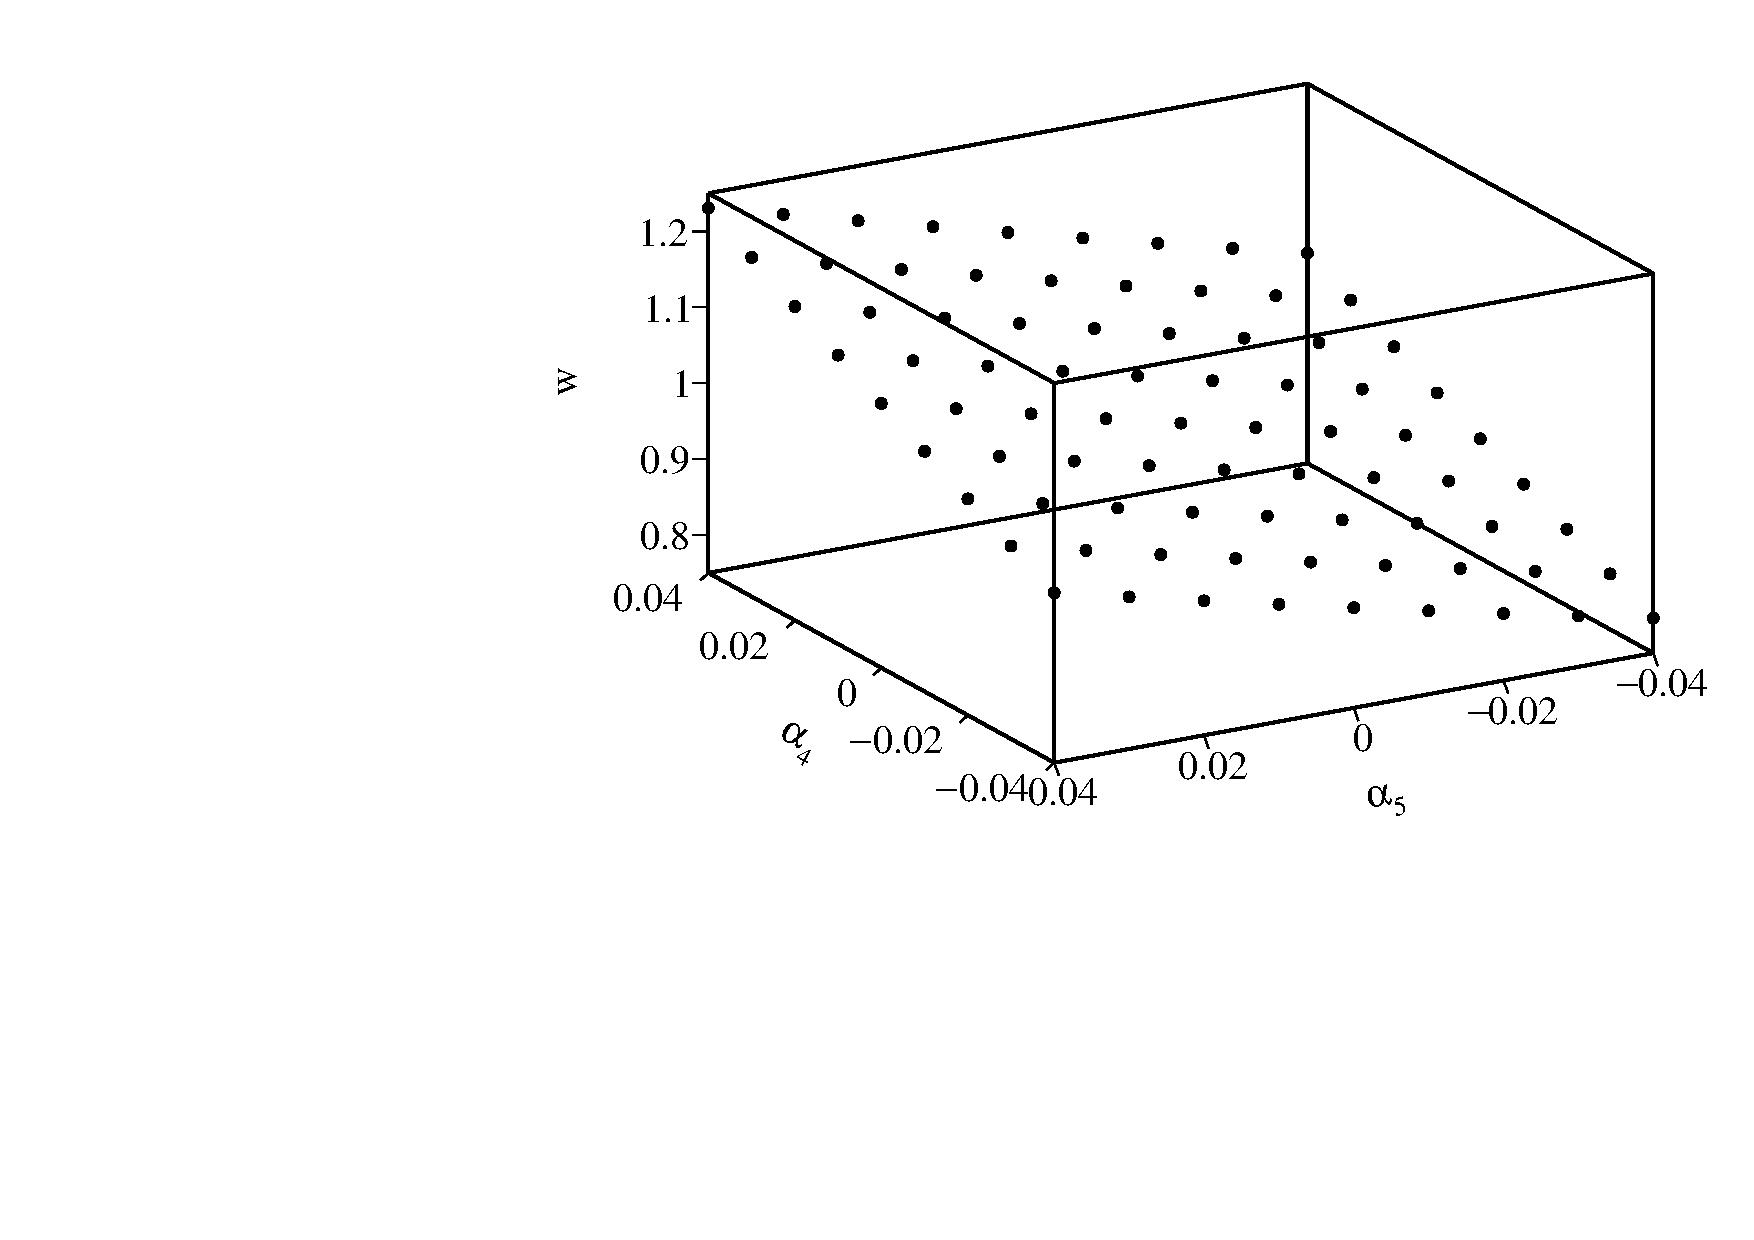
\includegraphics[width=0.5\textwidth]{PhysicsAnalysis/Plots/EventWeights/1400GeV/EventWeightsForEvent100001009_1400GeV_SPFOs_kt_0p70_10Bins_Start_0_End_10_1400GeV_Raw.pdf}}
\subfloat[]{\label{fig:weight2}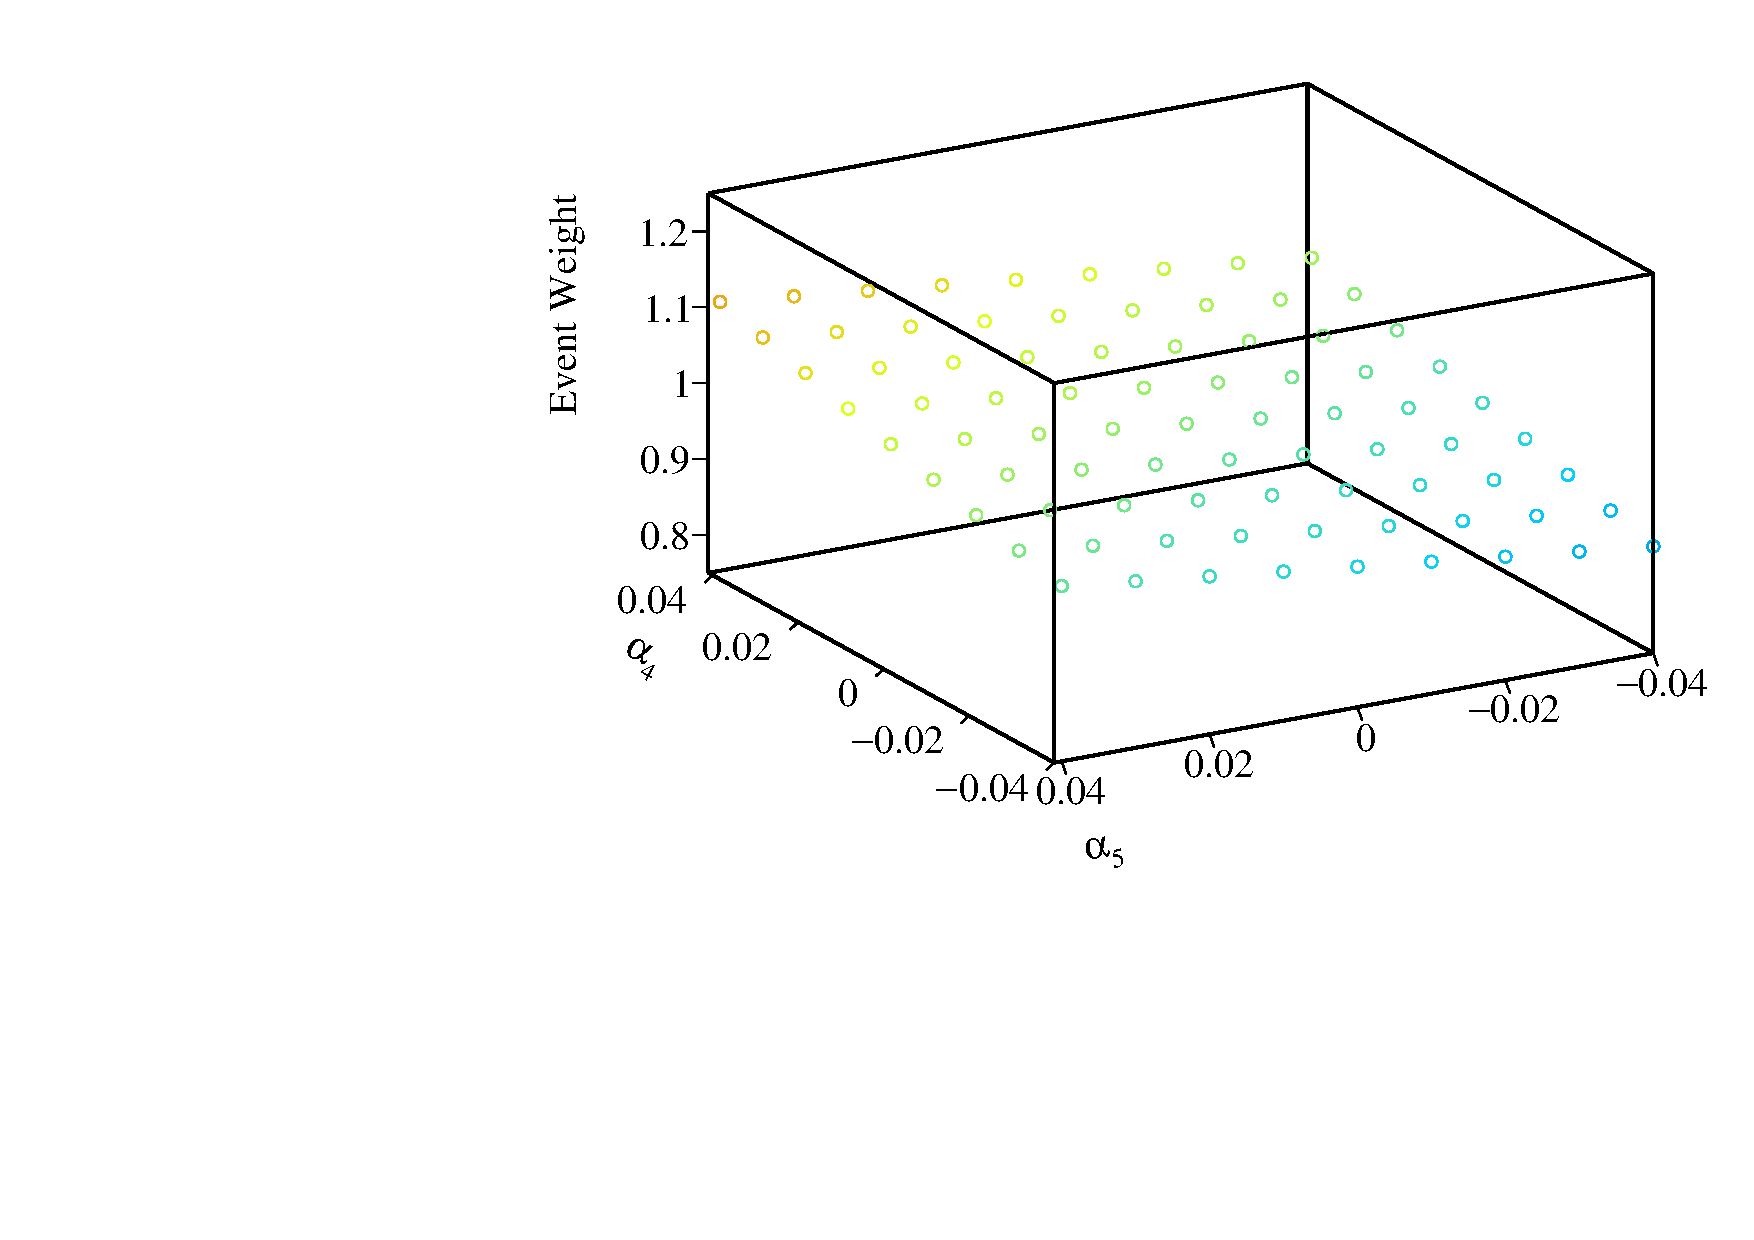
\includegraphics[width=0.5\textwidth]{PhysicsAnalysis/Plots/EventWeights/1400GeV/EventWeightsForEvent100001014_1400GeV_SPFOs_kt_0p70_10Bins_Start_0_End_10_1400GeV_Raw.pdf}} \hfill
\subfloat[]{\label{fig:weight3}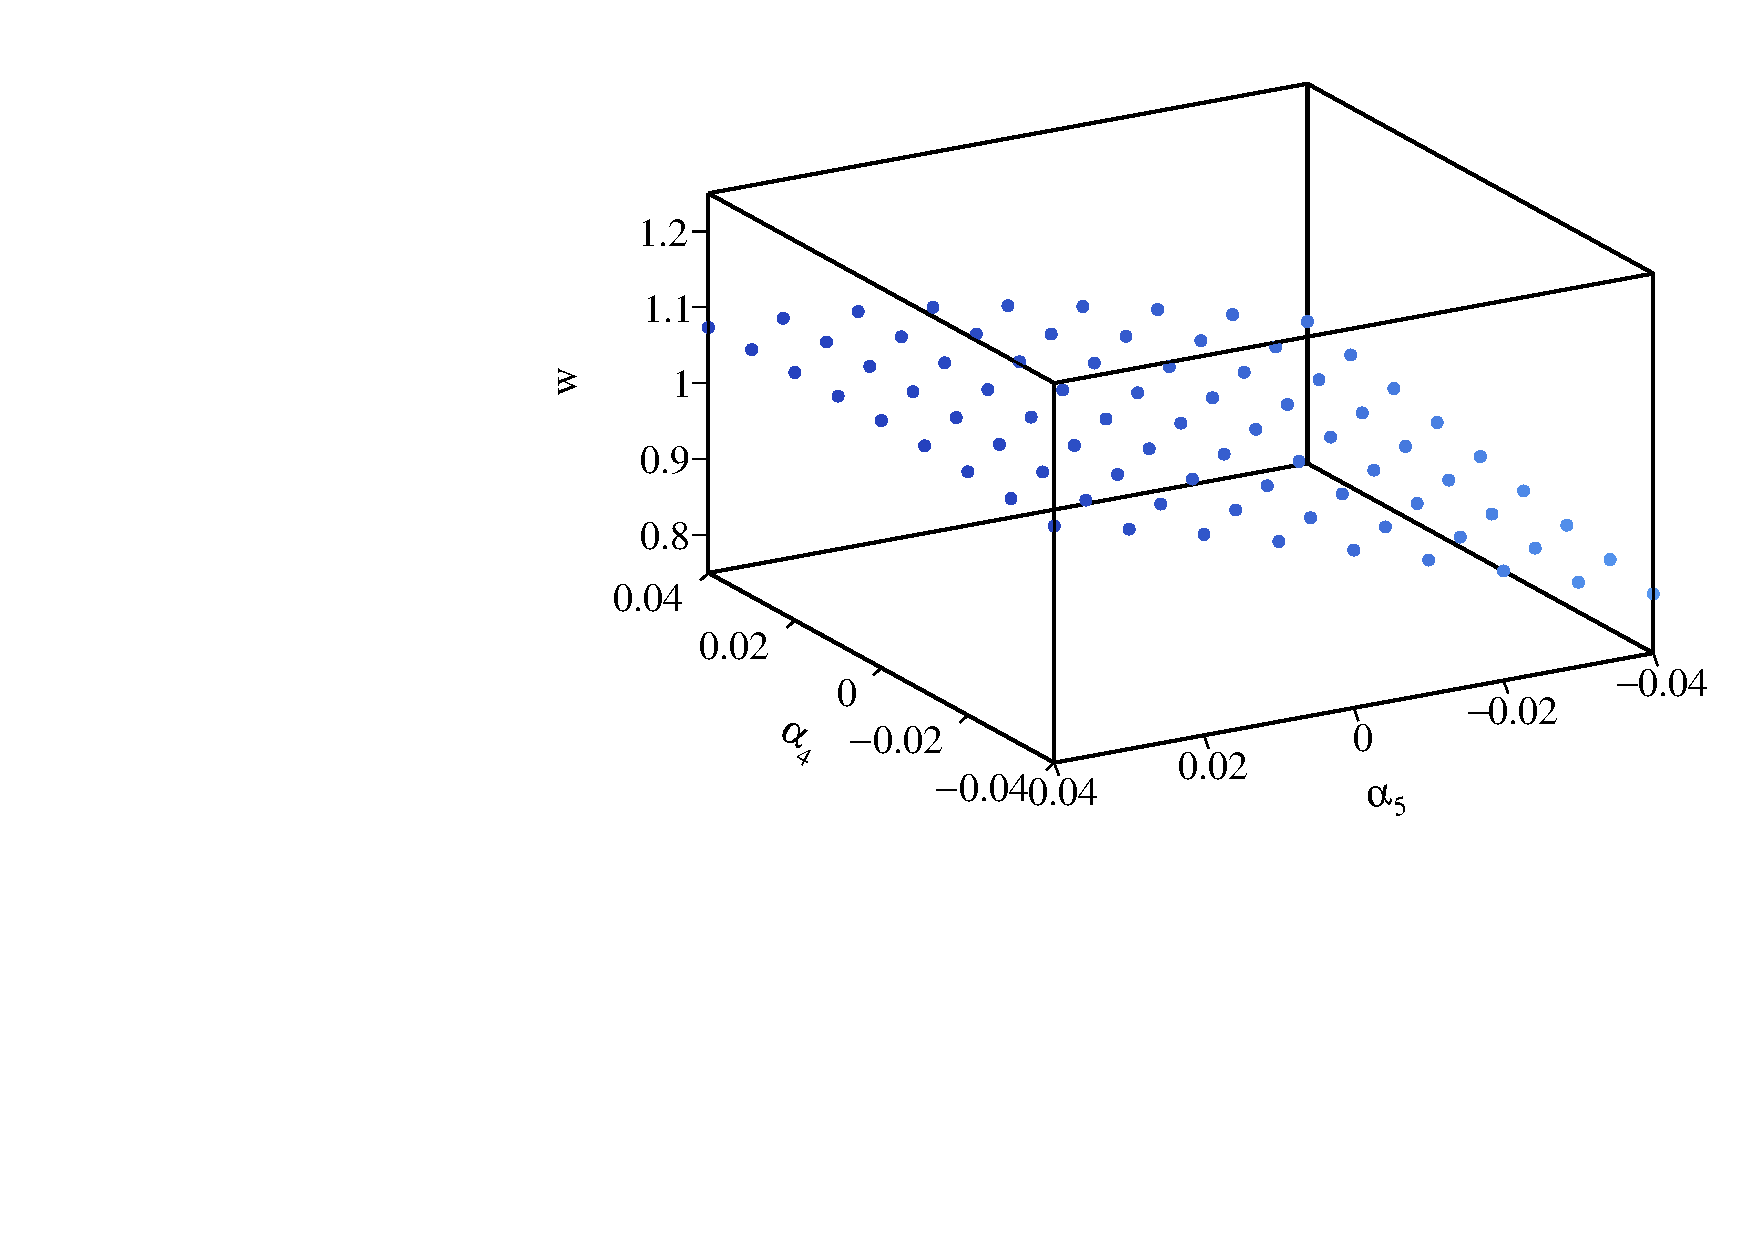
\includegraphics[width=0.5\textwidth]{PhysicsAnalysis/Plots/EventWeights/1400GeV/EventWeightsForEvent100001044_1400GeV_SPFOs_kt_0p70_10Bins_Start_0_End_10_1400GeV_Raw.pdf}}
\subfloat[]{\label{fig:weight4}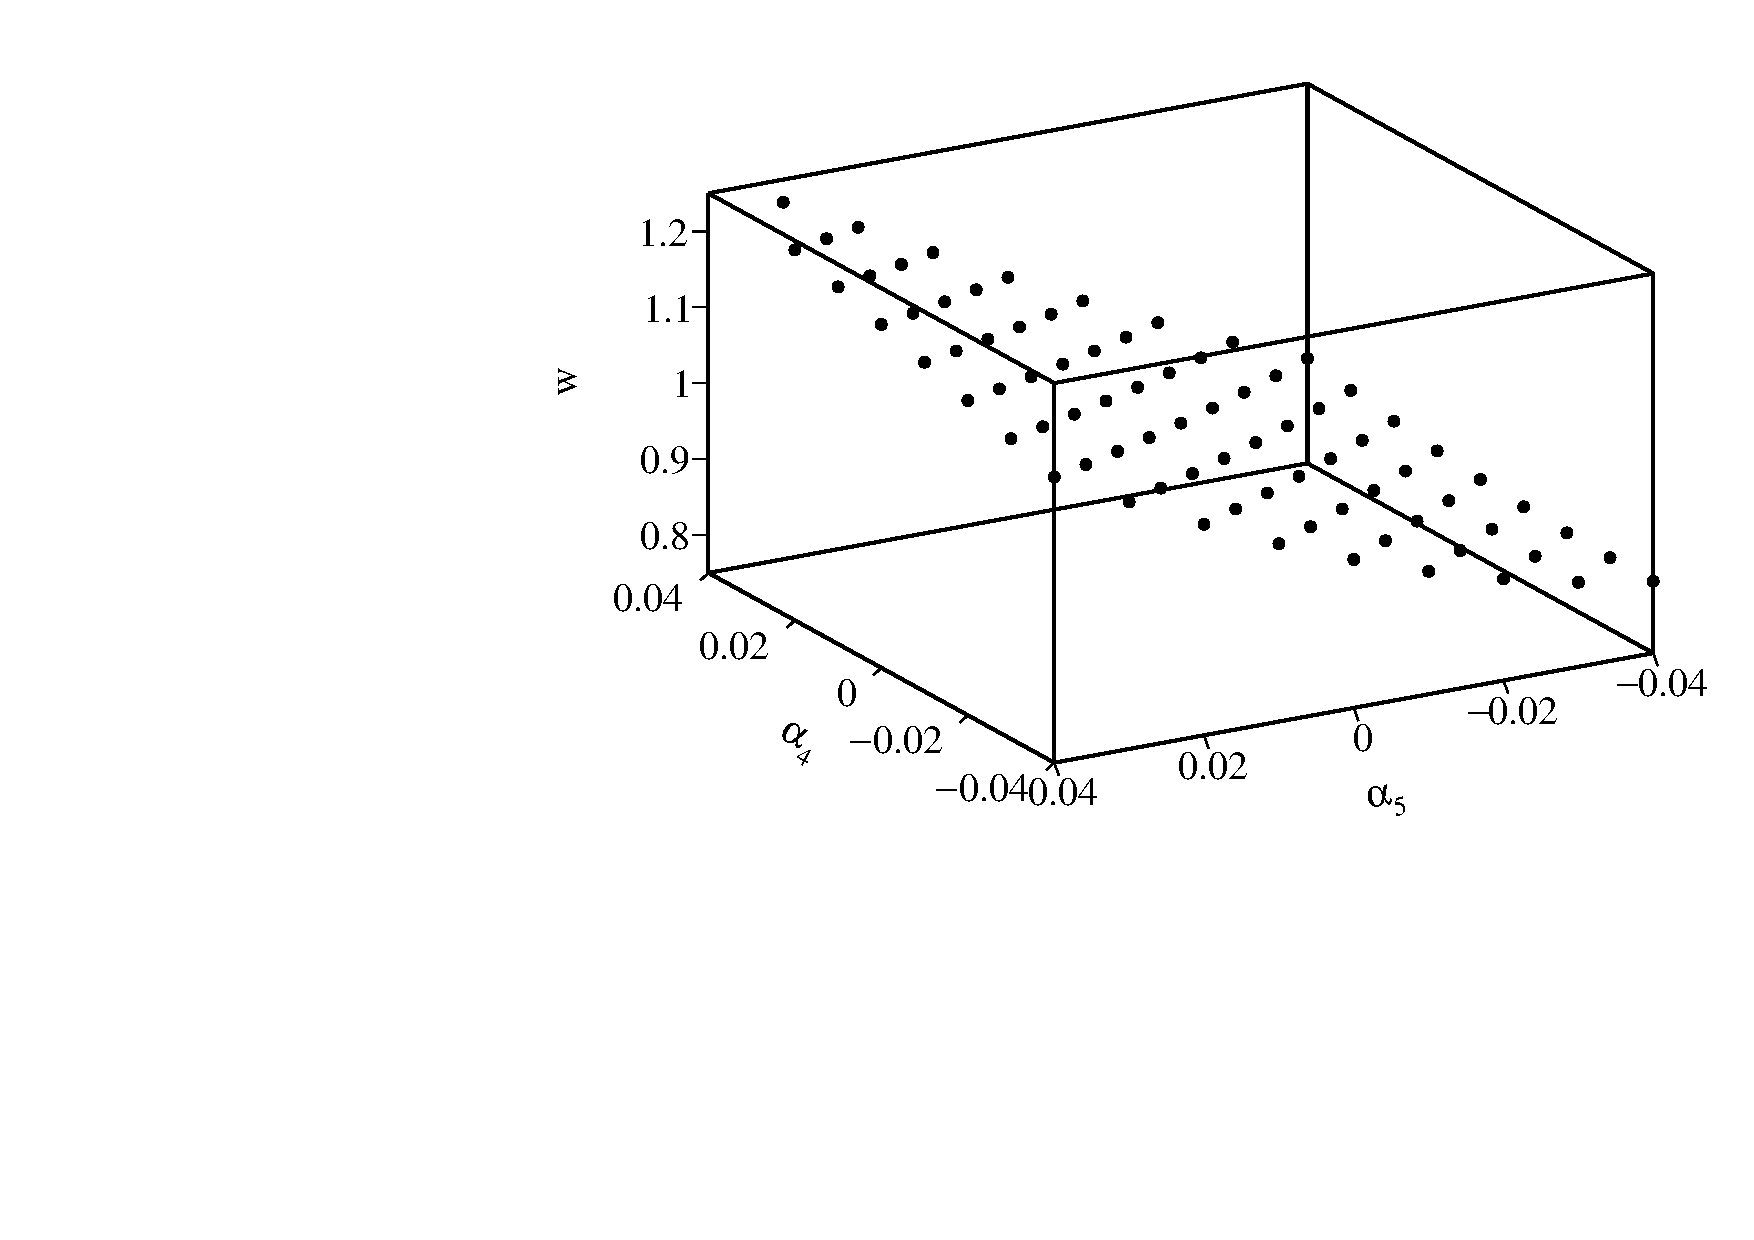
\includegraphics[width=0.5\textwidth]{PhysicsAnalysis/Plots/EventWeights/1400GeV/EventWeightsForEvent100001051_1400GeV_SPFOs_kt_0p70_10Bins_Start_0_End_10_1400GeV_Raw.pdf}}
\caption[The event weight as a function of the anomalous couplings $\alpha_{4}$ and $\alpha_{5}$ for a selection of \nu{\nu}qqqq final state events at 1.4~TeV.]{The event weight as a function of the anomalous couplings $\alpha_{4}$ and $\alpha_{5}$ for a selection of \nu{\nu}qqqq final state events at 1.4~TeV.}
\label{fig:eventweights1400raw}
\end{figure}

This reweighting procedure has many advantages over the alternative of generating new samples with fixed $\alpha_{4}$ and $\alpha_{5}$, notably the absence of systematic errors arising from new event generation, simulation and reconstruction.  Only final states showing a sensitivity to $\alpha_{4}$ and $\alpha_{5}$ require reweighting.  To determine those states a comparison was made between the cross section using the standard model values of $\alpha_{4}$ and $\alpha_{5}$, i.e. 0, and the same calculation using non-zero values of these couplings at 1.4~TeV.  This comparison was performed on all of the generated samples listed in table \ref{table:crosssection1400GeV} and the results for samples showing sensitivity to the couplings can be found in table \ref{table:crosssectionsensitivity1400}

\begin{table}[h!]
\centering
\begin{tabular}{ l r r r r }
\hline
Final State & Cross Section [fb] & Cross Section [fb] & Percentage \\ 
& ($\alpha_{4} = \alpha_{5} = 0.00$) & ($\alpha_{4} = \alpha_{5} = 0.05$) & Change[\%] \\ 
\hline
$\text{e}^{+}\text{e}^{-} \rightarrow \nu{\nu}\text{qqqq}$ & 24.7 & 34.6 & +40.1 \\
$\text{e}^{+}\text{e}^{-} \rightarrow \text{l}{\nu}\text{qqqq}$ & 115.3 & 113.0 & -2.0 \\
$\text{e}^{+}\text{e}^{-} \rightarrow \text{llqqqq}$ & 62.1 & 68.6 & +10.5 \\
\hline
\end{tabular}
\caption[Cross sections for selected processes showing the effect of the anomalous gauge couplings $\alpha_{4}$ and $\alpha_{5}$ at 1.4~TeV.]{Cross sections for selected processes showing the effect of the anomalous gauge couplings $\alpha_{4}$ and $\alpha_{5}$ at 1.4~TeV.}
\label{table:crosssectionsensitivity1400}
\end{table}

The cross sections were found to differ when using non-zero values for the anomalous couplings in comparison to the standard model prediction only for the vector boson scattering signal final states $\nu\nu\text{qqqq}$, $\text{l}\nu\text{qqqq}$ and llqqqq.  In reality, non-zero anomalous couplings would change the cross sections of all processes considered; however, the sensitivity would only arise from high order terms in the Lagrangian.  Such terms would not be dominant in determining the cross section and so are omitted from the generator making certain final states appear invariant to changes in the anomalous couplings.

The cross section calculations show that the most sensitive final state to the anomalous gauge couplings is \nu{\nu}qqqq; therefore, this analysis will focus entirely upon this final state.  As the l{\nu}qqqq final state has a much reduced sensitivity in comparison to the \nu{\nu}qqqq state and as the llqqqq can be easily vetoed from the analysis, as will be shown in subsequent chapters, it is only necessary to consider the sensitivity of the \nu{\nu}qqqq final state.  For the aforementioned reasons the l{\nu}qqqq and llqqqq final states will be treated as backgrounds that are invariant to changes in the anomalous couplings $\alpha_{4}$ and $\alpha_{5}$.  

In order to determine the anomalous gauge coupling sensitive event weights, it was necessary to use the anomalous gauge coupling model in Whizard, however, this enforced a unit CKM matrix.  This has a negligible impact on this analysis as no significant differences were observed when comparing a variety of reconstructed level distributions for samples of \nu{\nu}qqqq generated with a standard model and a unit CKM matrix.  Furthermore, flavour tagging of jets was not used in this analysis as it offered negligible gains when performing event selection, which means any differences in quark flavour due to the unit CKM matrix for the \nu{\nu}qqqq final state should be irrelevant.

%========================================================================================
%========================================================================================

\section{Data Analysis}
\label{sec:dataanalysis}
The focus of this section is to describe the post reconstruction procedure applied to the signal and background events, described in \ref{sec:eventgenerationandbackgrounds}, to extract the relevant information needed for the sensitivity study. 

%========================================================================================

\subsection{Jet Finding} 
\label{sec:jetpairing}
After the standard reconstruction, described in chapter \ref{chap:reconstructionchain}, two further processors are applied to remove reconstructed particle flow objects (PFOs) that originate from beam related backgrounds, also described in chapter \ref{chap:reconstructionchain}, from the event.  The first processor, the CLICTrackSelection, is designed to veto poorly reconstructed tracks and to reject tracks where the time of arrival at the calorimeter when comparing a helix fit to the track and a straight line of flight differ by 50ns.  The latter would indicate the tracked particle does not create the calorimetric energy deposits that it has been associated to.  The second processor, the CLICPfoSelector, applies cuts to the $p_{\text{T}}$ and timing information of the PFOs.  These cuts vary as a function of position in the detector and the reconstructed particle type to target regions of the detector where backgrounds are more prominent, primarily low $p_{\text{T}}$ from $\gamma\gamma \rightarrow \text{Hadrons}$ events.  Three configurations of the CLICPfoSelector have been developed for the CLIC environment and were considered for this analysis.  They are, in order of increasing background rejection, the Loose, Default and Tight selections. The full details of each can be found here \cite{arXiv:1209.4039}.

After the application of the CLICTrackSelection and CLICPfoSelector the MarlinFastJet processor, a wrapper for the FastJet \cite{Cacciari:2011ma} processor, was used to cluster the events into four jets.  These jets are then paired up to form two candidate bosons.  This pairing is performed on the assumption that the correct pairing is achieved when the difference between the invariant masses of the candidate bosons is a minima.  In the case of the signal final state, $\nu\nu$qqqq, it is assumed that the four jets and two candidate bosons map onto the four quarks and the two outgoing bosons involved in the vector boson scattering process.  The jet clustering was done using the longitudinally invariant $k_{t}$ jet algorithm in exclusive mode.  In contrast to the inclusive mode, the exclusive mode allows the user to request a fixed number of jets in the output from MarlinFastJet.  The longitudinally invariant $k_{t}$ algorithm proceeds as follows:

\begin{itemize}
\item For each pair of particles, $i$ and $j$, the $k_{t}$ distance, $d_{ij}$, and beam distance, $d_{iB} = p_{t}^{2}$, are calculated.  $d_{ij}$ is defined as:
\begin{equation}
d_{ij} = \text{min}(p_{ti}^{2}, p_{tj}^{2}){\Delta}R^{2}_{ij}/R^{2}
\end{equation}
where ${\Delta}R^{2}_{ij} = (y_{i} - y_{j})^2 + (\phi_{i} - \phi_{j})^2$, $p_{t}$ is the transverse momentum of the particle with respect to the beam axis, $y_{i}$ is the rapidity of particle i and $\phi_{i}$ is the azimuthal angle of particle $i$. $R$ is a configurable parameter that typically is of the order of 1.
\item The minimum distance, $d_\text{min}$, of all the $k_{t}$ and beam distances is found.  If the minimum occurs for a $k_{t}$ distance, particles $i$ and $j$ are merged, summing their 4-momenta.  If the beam distance is the minima, particle $i$ was declared to be part of the "beam" jet and the particle is removed from the list of particles and not included in the final jet output.
\item This is repeated until the desired number of jets was created.  Alternatively, in inclusive mode this would be repeated until no particles are left in the event.
\end{itemize}

Two other clustering algorithms were considered, but, as figure \ref{fig:invariantmassalgoveto} shows, were found to be inappropriate for the experimental conditions at CLIC.  These alternative algorithm choices are applied in the same manor as the longitudinally invariant $k_{t}$ algorithm, however, they differ in the definition of $d_{ij}$ and $d_{iB}$.

\begin{figure}[h!]
\centering
\subfloat[]{\label{fig:invariantmassalgoveto1400GeV}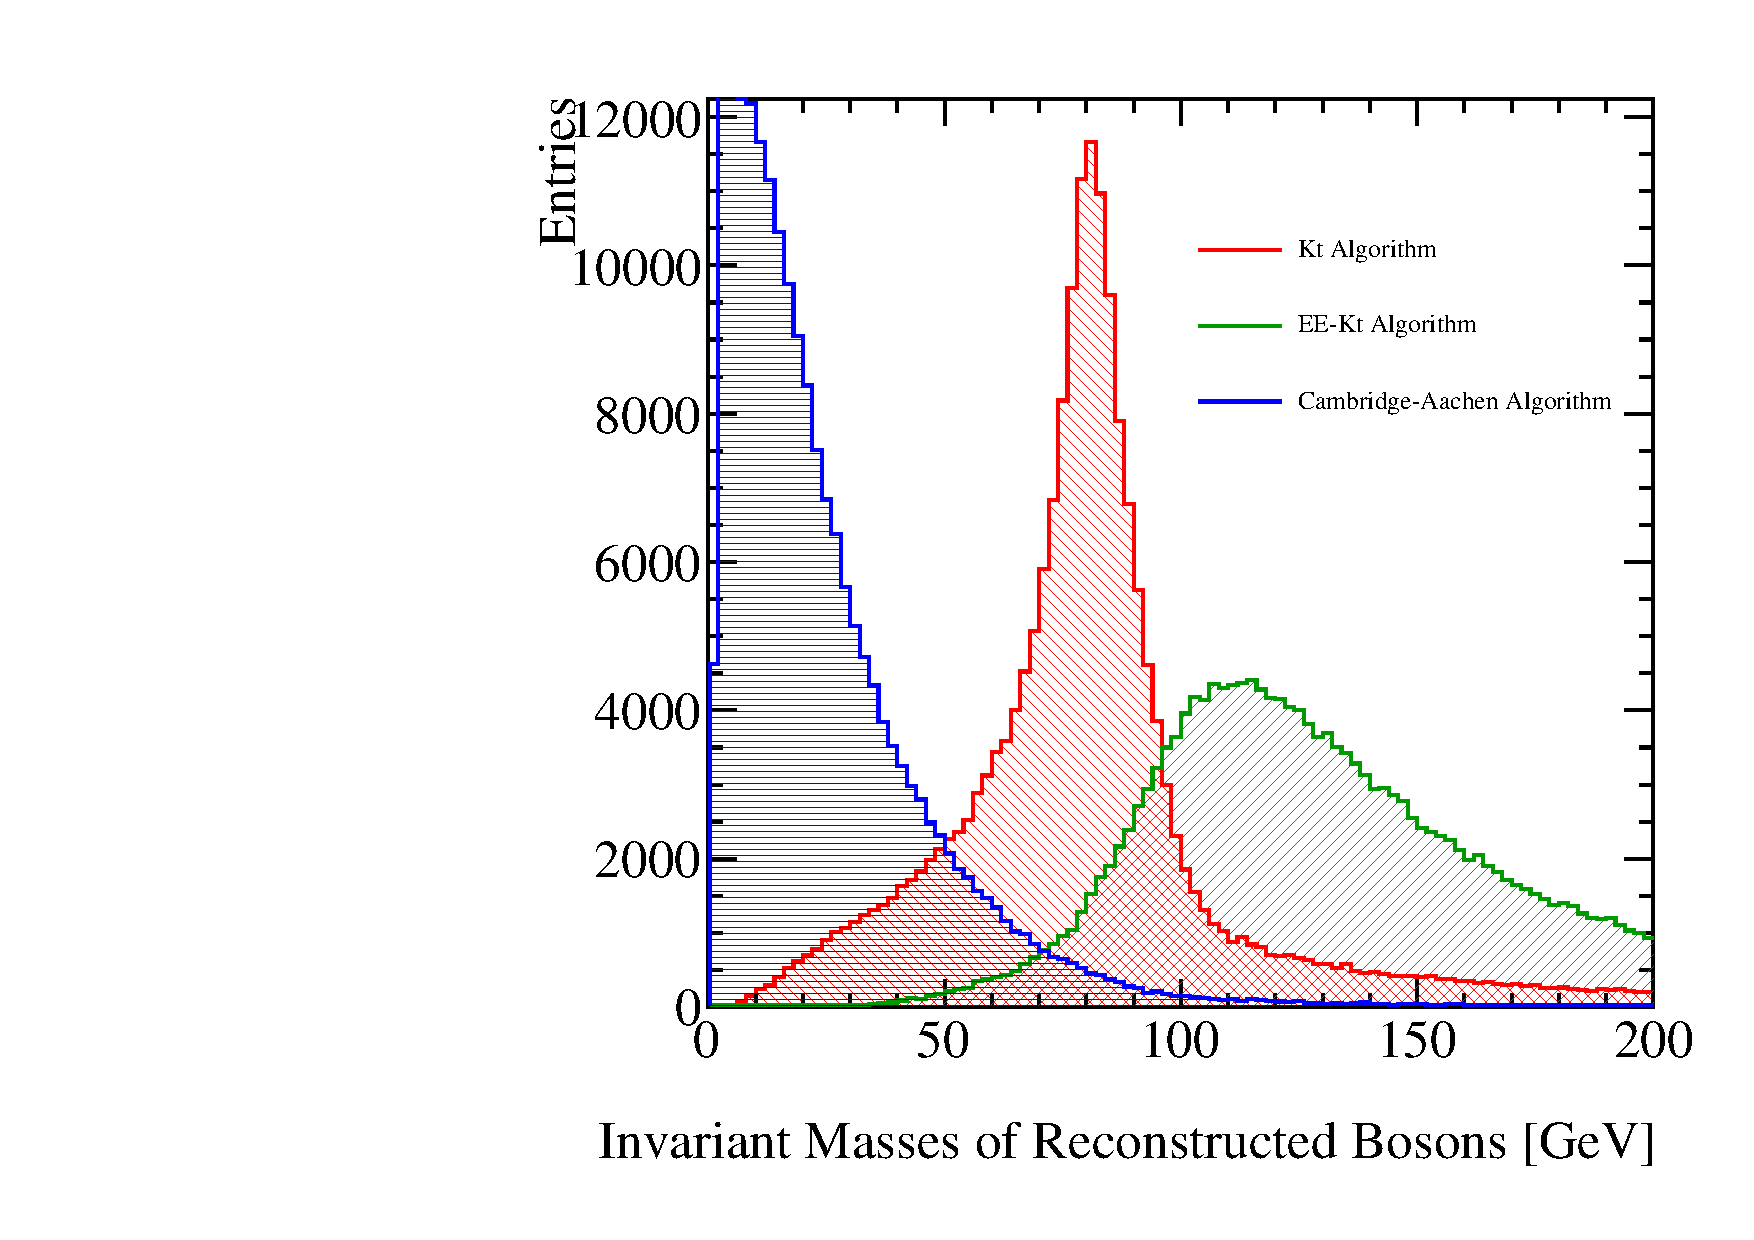
\includegraphics[width=0.5\textwidth]{PhysicsAnalysis/Plots/SimpleInvMassPlot/InvariantMassesAlgorithmVeto.pdf}}
\caption[The reconstructed masses for different choices of jet algorithm for 1.4~TeV \nu{\nu}qqqq final state events.  The masses are determined by forcing the events into 4 jets and then pairing the jet pairs to form candidate bosons.  The jet pairing configuration is determined by pairing jets such that the mass differences between the two candidate bosons is a minimum.  These samples should be dominated by vector boson scattering involving pairs of outgoing W bosons and so it is expected that a peak at the W boson mass, $m_{W} = 80.385 \pm 0.015$~GeV \cite{Beringer:1900zz}, should be observed.  As this does not occur for the Cambridge-Aachen algorithm or the EE\_kt algorithm they were deemed unsuitable for this analysis. In the case of the kt algorithm and the EE\_kt algorithm an R parameter of 0.7 was used.]{The reconstructed masses for different choices of jet algorithm for 1.4~TeV \nu{\nu}qqqq final state events.  The masses are determined by forcing the events into 4 jets and then pairing the jet pairs to form candidate bosons.  The jet pairing configuration is determined by pairing jets such that the mass differences between the two candidate bosons is a minimum.  These samples should be dominated by vector boson scattering involving pairs of outgoing W bosons and so it is expected that a peak at the W boson mass, $m_{W} = 80.385 \pm 0.015$~GeV \cite{Beringer:1900zz}, should be observed.  As this does not occur for the Cambridge-Aachen algorithm or the EE\_kt algorithm they were deemed unsuitable for this analysis. In the case of the kt algorithm and the EE\_kt algorithm an R parameter of 0.7 was used.}
\label{fig:invariantmassalgoveto}
\end{figure}

The first alternative jet algorithm considered was the $k_{t}$ algorithm for $\text{e}^{+}\text{e}^{-}$ colliders, the EE\_kt or Durham algorithm, where $d_{ij} = 2\text{min}(E_{i}^{2}, E_{j}^{2})(1-cos\theta_{ij})$ and $d_{iB}$ is not used.  $\theta_{ij}$ is the opening angle of particles $i$ and $j$ meaning that in the collinear limit $d_{ij}$ corresponds to the relative transverse momenta of the particles.  The major failure of this algorithm when applied to CLIC is the absence of $d_{iB}$, which leads to many beam related background particles being associated to jets.  As figure \ref{fig:invariantmassalgoveto} shows, the invariant mass of the paired jets, which should peak around the W and Z boson masses, is much larger than expected, due to the presence of the beam related backgrounds in the jets.  Also this algorithm is not invariant to boosts along the beam direction making it inappropriate to use at CLIC as the beam induced backgrounds modify the nominal collision kinematics.  

The second alternative jet algorithm considered was the Cambridge-Aachen jet algorithm where $d_{ij} = {\Delta}R_{ij}^{2}/R^2$ and $d_{iB} = 1$.  This algorithm performed poorly as it does not accounts for the transverse momentum or the energy of the particles being clustered. In essence, this is a cone clustering algorithm with a cone radius defined through ${\Delta}R_{ij} = R$, which even for large R was found to discard too much energy in the event to be useful for this analysis.  This can be seen in figure \ref{fig:invariantmassalgoveto} where the invariant mass of the paired jets is much lower than expected.  This algorithm is appropriate for events that contain highly boosted jets, however, at CLIC the jets are too disperse for this algorithm to be successful.

%========================================================================================

\subsubsection{Optimal Jet Finding Algorithm}
\label{sec:optimaljetalgorithm}
Optimisation of the jet finding procedure was performed on both the PFO selection, described in section \ref{sec:jetpairing}, and the value of the R parameter used in the longitudinally invariant $k_{t}$ algorithm.   The optimal configuration for the jet algorithm at 1.4~TeV was found to use default selected PFOs and an R parameter of 0.9.

The optimisation procedure involved performing the sensitivity study, described in section \ref{sec:fitting}, using solely the {\nu}{\nu}qqqq signal final state.  This led to the construction of a $\chi^{2}$ surface from which confidence contours can be extracted in the $\alpha_{4}$ and $\alpha_{5}$ space.  The $\chi^{2}$ surface was constructed by comparing the distribution of the invariant mass of the visible system, $M_{VV}$, with and without the effect of the anomalous couplings $\alpha_{4}$ and $\alpha_{5}$.  The $\chi^{2}$ surface for the optimal jet configuration at 1.4~TeV using the {\nu}{\nu}qqqq signal final state is shown in figure \ref{fig:chi2jetalgoideal1400GeV}.  This methodology ensured that the optimisation was done with respect to the physics of interest without having to perform the jet reconstruction for the large number of background events for each jet algorithm configuration considered.  

Confidence limits on the individual parameters $\alpha_{4}$ and $\alpha_{5}$ were determined by setting the corresponding coupling term to zero and examining the one dimensional $\chi^{2}$ distribution.  A fourth order polynomial was fitted to the minima of this distribution and the one sigma confidence limit defined using $\Delta\chi^{2}$ of 1.  $\Delta\chi^{2}$ is defined as the change in $\chi^{2}$ with respect to the minima in the $\chi^{2}$ surface.  Note that for the two dimensional $\chi^{2}$ surface a one sigma confidence limit is given by a $\Delta\chi^{2}$ of 2.28 due to the additional degree of freedom in the fit.  The one dimensional $\chi^{2}$ distribution for $\alpha_{4}$ and $\alpha_{5}$, assuming $\alpha_{5} = 0$ and $\alpha_{4} = 0$ respectively, for the optimal jet configuration at 1.4~TeV using the {\nu}{\nu}qqqq signal final state is shown in figures \ref{fig:a4chi2jetalgoideal1400GeV} and \ref{fig:a5chi2jetalgoideal1400GeV}.  Using these distributions the one sigma confidence limits on $\alpha_{4}$ are -0.0038 to 0.0047 and on $\alpha_{5}$ are -0.0027 to 0.0030.

\begin{figure}
\centering
\subfloat[]{\label{fig:chi2jetalgoideal1400GeV}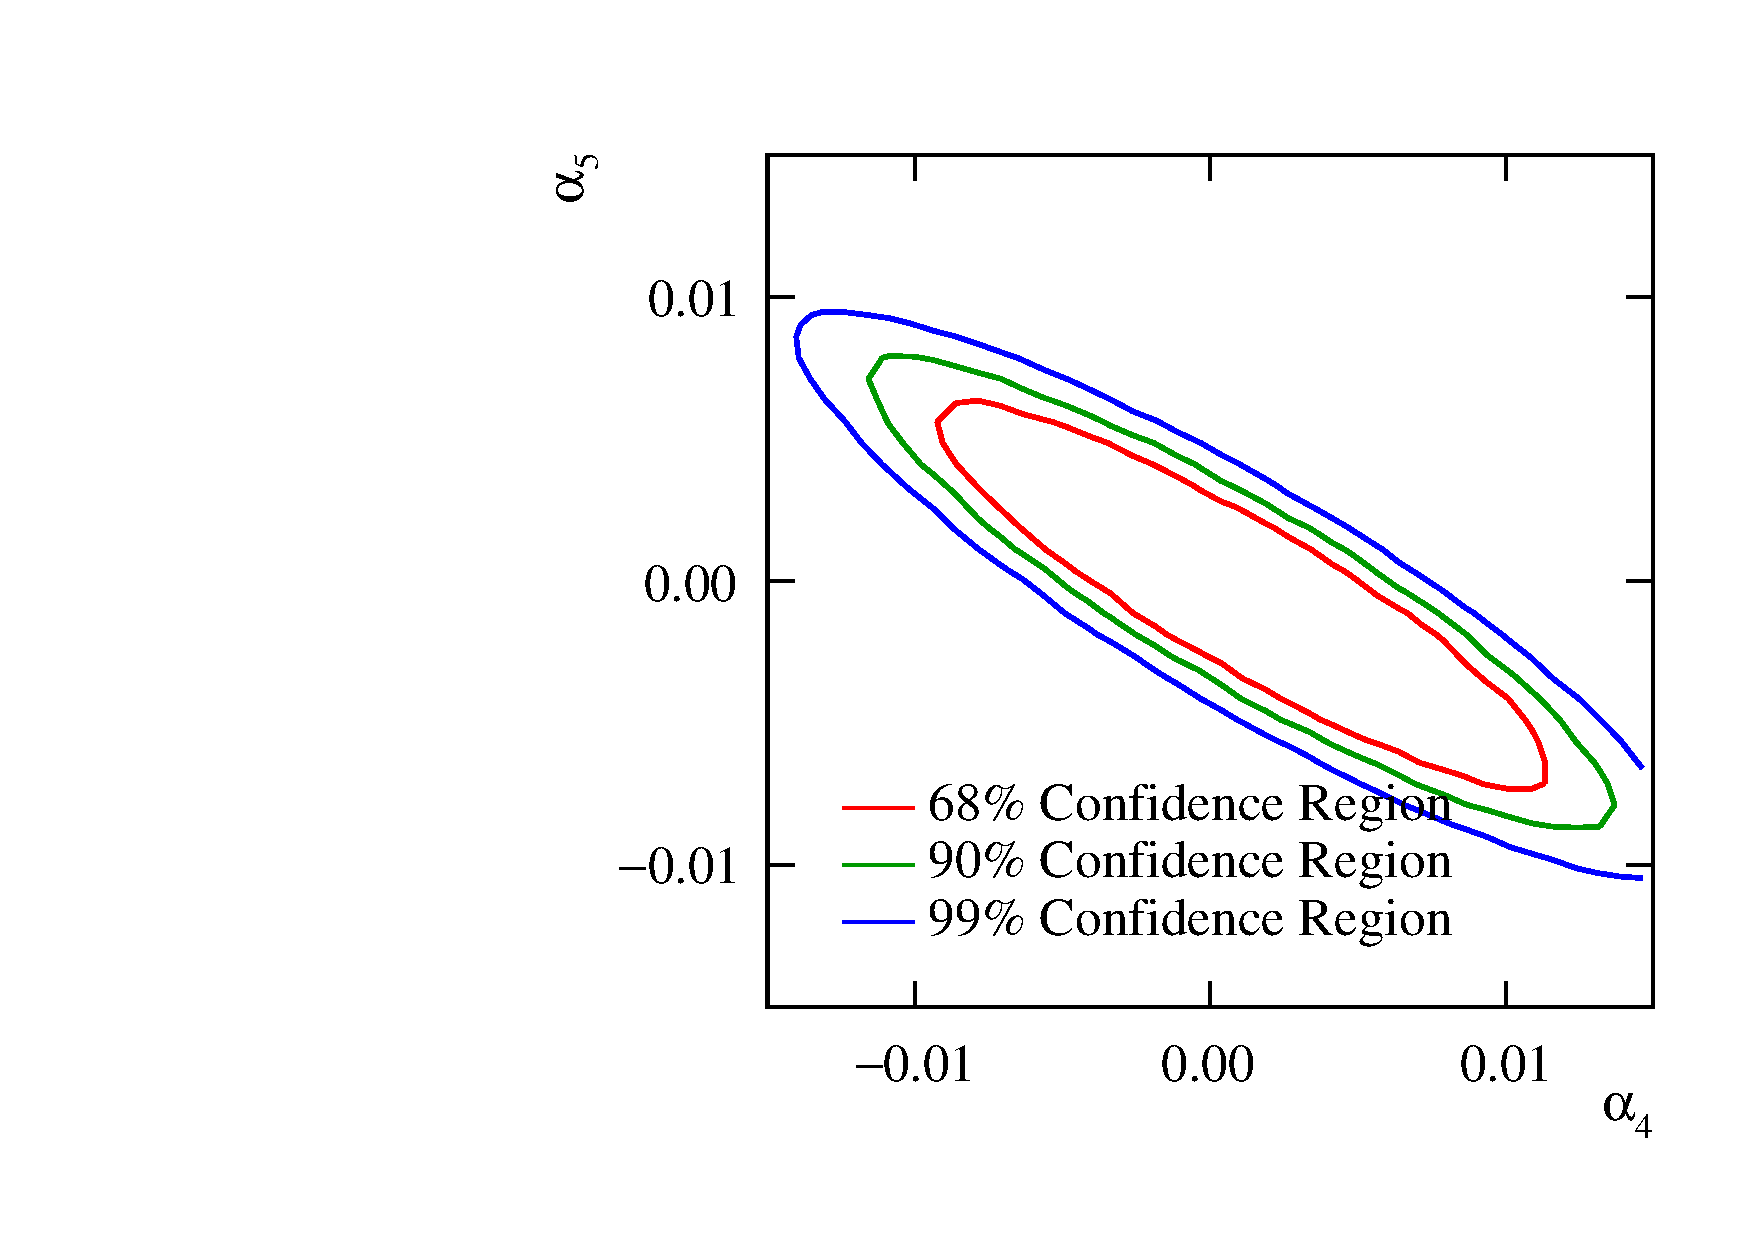
\includegraphics[width=0.5\textwidth]{PhysicsAnalysis/Plots/Chi2ContoursOptimisation/1400GeV/KtSPFOsR0p90_Optimal.pdf}}\hfill
\subfloat[]{\label{fig:a4chi2jetalgoideal1400GeV}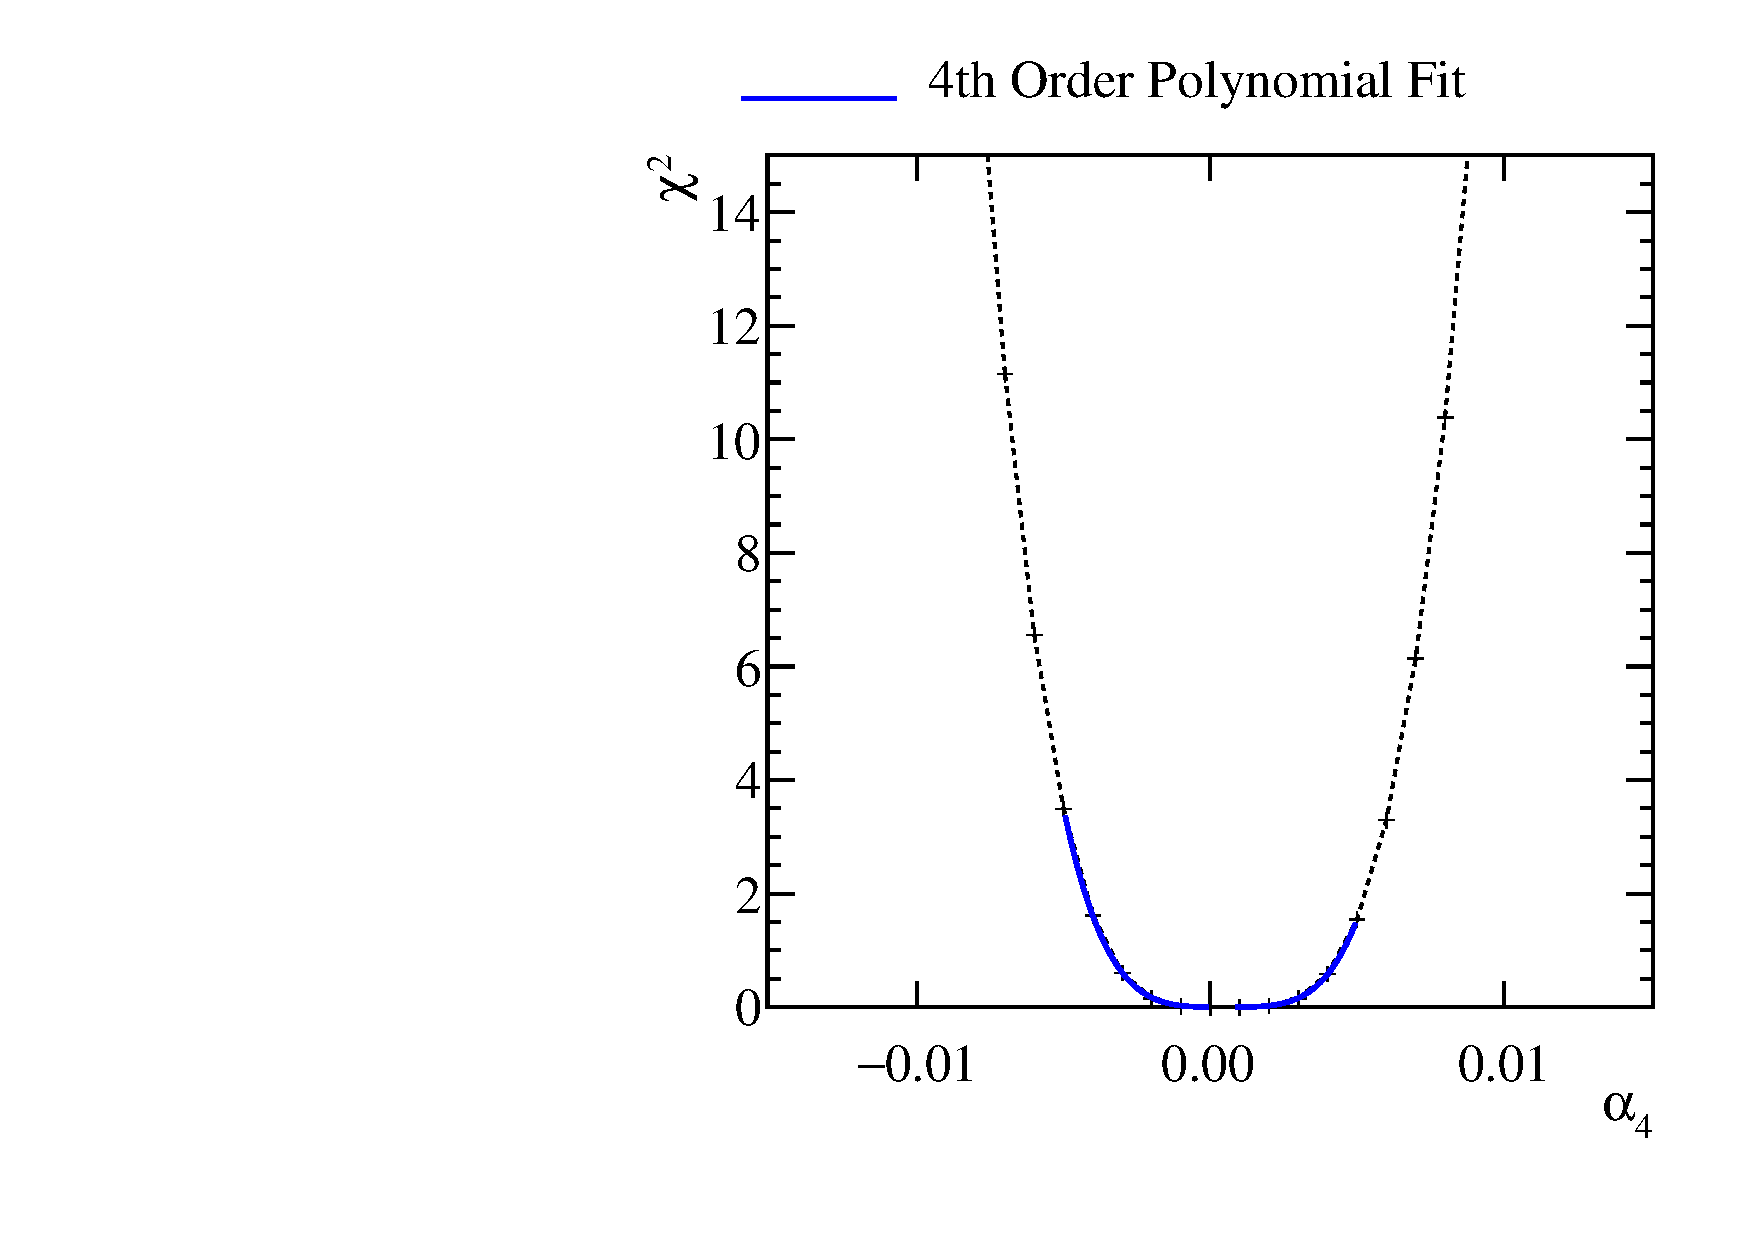
\includegraphics[width=0.5\textwidth]{PhysicsAnalysis/Plots/Chi2ContoursOptimisation/1400GeV/KtSPFOsR0p90_alpha4_Optimal.pdf}}
\subfloat[]{\label{fig:a5chi2jetalgoideal1400GeV}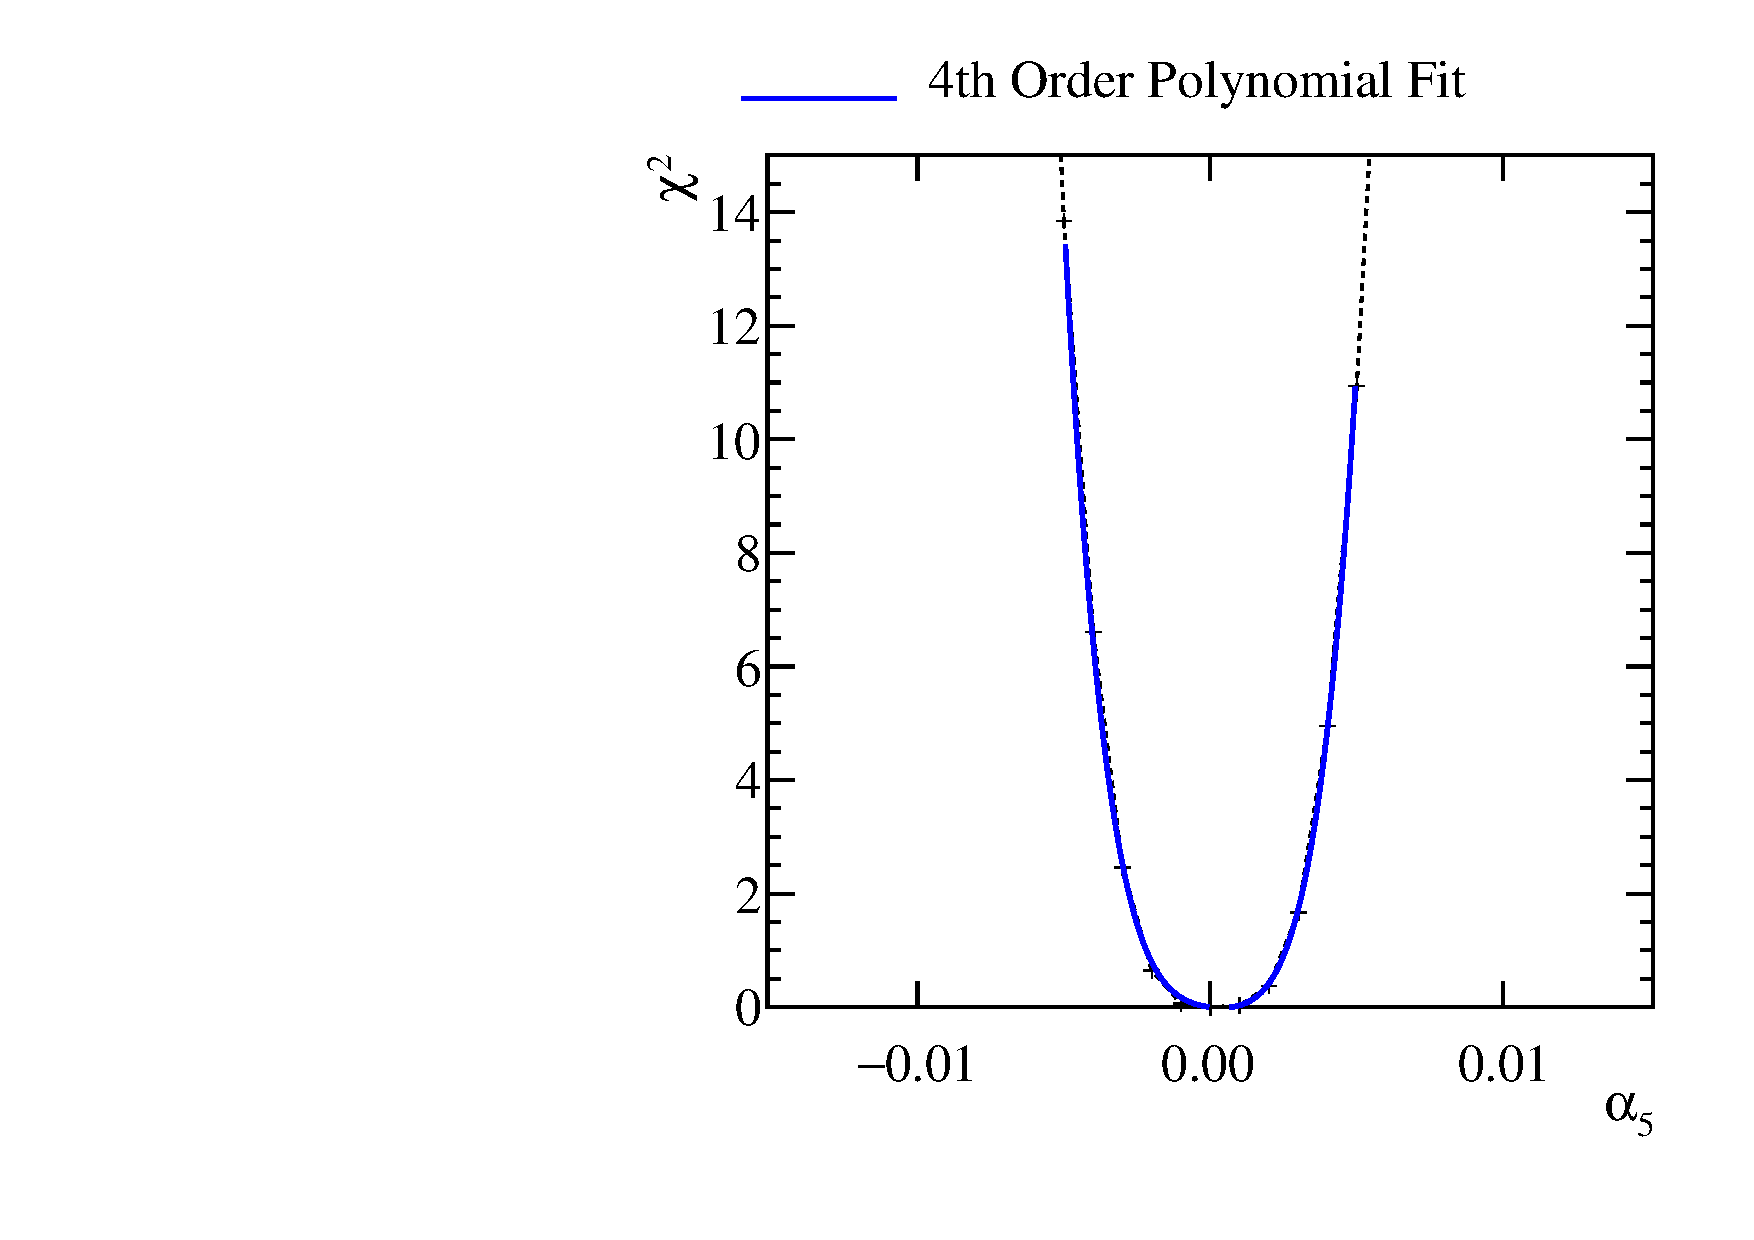
\includegraphics[width=0.5\textwidth]{PhysicsAnalysis/Plots/Chi2ContoursOptimisation/1400GeV/KtSPFOsR0p90_alpha5_Optimal.pdf}}
\caption[$\chi^{2}$ sensitivity distributions from a fit to $M_{VV}$ for the signal $\text{qqqq}\nu\nu$ final state only at 1.4~TeV.  These results use the optimal jet algorithm configuration of selected PFOs and an R parameter of 0.9 in the $k_{t}$ algorithm.  \protect\subref{fig:chi2jetalgoideal1400GeV} $\chi^{2}$ sensitivity contours in $\alpha_{4}$ and $\alpha_{5}$ space.  \protect\subref{fig:a4chi2jetalgoideal1400GeV} $\chi^{2}$ as a function of $\alpha_{4}$ assuming $\alpha_{5} = 0$.  \protect\subref{fig:a5chi2jetalgoideal1400GeV} $\chi^{2}$ as a function of $\alpha_{5}$ assuming $\alpha_{4} = 0$.]{$\chi^{2}$ sensitivity distributions from a fit to $M_{VV}$ for the signal $\text{qqqq}\nu\nu$ final state only at 1.4~TeV.  These results use the optimal jet algorithm configuration of selected PFOs and an R parameter of 0.9 in the $k_{t}$ algorithm.  \protect\subref{fig:chi2jetalgoideal1400GeV} $\chi^{2}$ sensitivity contours in $\alpha_{4}$ and $\alpha_{5}$ space.  \protect\subref{fig:a4chi2jetalgoideal1400GeV} $\chi^{2}$ as a function of $\alpha_{4}$ assuming $\alpha_{5} = 0$.  \protect\subref{fig:a5chi2jetalgoideal1400GeV} $\chi^{2}$ as a function of $\alpha_{5}$ assuming $\alpha_{4} = 0$.}
\label{fig:allchi2jetalgoideal1400GeV}
\end{figure}

%========================================================================================

\subsection{Lepton Finding} 
\label{sec:isolatedleptonfinding}
An isolated lepton finder was included in the analysis chain in an attempt to reject background final states containing leptons.  As it is unlikely that isolated leptons will form via hadronisation, because all hadronisation products are boosted along the direction of the parent quark, it is likely that they originate from the primary interaction occurring at the IP.  This makes the number of isolated leptons a powerful discriminating variable for discerning final states containing leptons. 

The isolated lepton finder attempts to find whether a PFO is an electron or muon based on the calorimetric energy deposits.  If the calorimetric energy deposits for a PFO are consistent with that of an electron or muon and there is a single associated track then cuts are placed on that that associated track to determine whether the track originates from the IP.  If the track cuts deem the PFO to have originated from the IP, isolation cuts restricting the energy deposited in the calorimeters within a cone surrounding the PFO are applied to ensure the particles does not belong to a jet.  If a PFO passes all of these criteria then it is counted as an isolated lepton.  The efficiency of the lepton finder is summarised in table \ref{table:efficiencyleptonfinding}.   

\begin{table}[h!]
\centering
\begin{tabular}{ l r }
\hline
Final State & $\epsilon_{\text{Lepton Finding}}$ \\ 
\hline
$\text{e}^{+}\text{e}^{-} \rightarrow \nu{\nu}\text{qqqq}$ & 99.7 \\
$\text{e}^{+}\text{e}^{-} \rightarrow \text{l}\nu\text{qqqq}$ & 48.9 \\
\hline
\end{tabular}
\caption[The efficiency of isolated lepton finding at 1.4~TeV for the {\nu}{\nu}qqqq and l{\nu}qqqq final states.]{The efficiency of isolated lepton finding at 1.4~TeV for the {\nu}{\nu}qqqq and l{\nu}qqqq final states.  Efficiency here is defined as the fraction of events where no isolated leptons were found.}
\label{table:efficiencyleptonfinding}
\end{table}

%========================================================================================

\subsection{Discriminant Variables} 
\label{sec:analysisprocessor}
The next stage of the analysis involved the calculation of a number of event-based variables that were found to be useful for this analysis.  The variables that were calculated are as follows:

\begin{itemize}
\item \textbf{Particle level} variables:

\begin{itemize}
\item Number of PFOs in each jet.
\item Energy of the highest energy PFO.
\item Energy of the highest energy electron.
\item Cosine of the polar angle of the highest energy track.
\item The number of isolated leptons found using the isolated lepton finder.
\end{itemize}

\item \textbf{Candidate boson} variables:

\begin{itemize}
\item Energy of the candidate bosons.
\item Invariant mass of the candidate bosons.
\item Acolinearity of the candidate boson pair, which is defined as 180 degrees minus the opening angle of the pair of bosons in the rest frame of the detector.
\end{itemize}

\item \textbf{Event based} variables:  

\begin{itemize}
\item The invariant mass of the visible system, $M_{VV}$.
\item The vector sum of the transverse momentum of all PFOs in the event. 
\item Sphericity, defined through the sphericity tensor $S^{ab}$:
\begin{equation}
S^{ab} = \frac{\Sigma_{i}p^{\alpha}_{i}p^{\alpha}_{j}}{\Sigma_{i,\alpha=1,2,3}|p^{\alpha}_{i|^{2}}}
\end{equation}
Where $p_{i}$ are the components of the momenta of PFO $i$ in the rest frame of the detector and the sum $\Sigma_{i}$ runs over all particles in the event.  Sphericity is defined as $\text{S} = \frac{3}{2}(\lambda_{2} + \lambda_{3})$, where $\lambda_{i}$ are the eigenvalues of the sphericity tensor defined such $\lambda_{1} \geq \lambda_{2} \geq \lambda_{3}$.  This provides a measure of how spherical the reconstructed event topology is with isotropic events having $S \approx 1$, while two jet events have $S \approx 0$.
\end{itemize}

\item \textbf{Jet clustering parameter} variables, $y_{ij}$ where $i = 3,4$ and $j=i+1$.  These are the smallest $k_{t}$ distance found when combining $j$ jets into $i$ jets.  The variable used in the multivariate analysis is $-\text{log}_{10}(y_{ij})$.
\end{itemize}

%========================================================================================
%========================================================================================

\section{Event Selection}
\label{sec:eventselection}
As described in section \ref{sec:modellingofanomalouscouplings}, the signal for this analysis is the \nu{\nu}qqqq final state, while the backgrounds consist of all two and four jet final states that could be confused with the signal after reconstruction.  A complete list of signal and background final states used for this analysis, alongside their standard model cross sections, can be found in table \ref{table:crosssection1400GeV}.  In an attempt to isolate the signal final state from the backgrounds an event selection procedure consisting of a set of preselection cuts followed by the application of a multivariate analysis (MVA), was applied.  The full details of this procedure are given in the following section.  All event numbers used in this analysis have been normalised, prior to event selection, to the correct luminosity for CLIC running at 1.4~TeV.

%========================================================================================

\subsection{Preselection}
\label{sec:preselection1400GeV}
A refined selection of the \nu{\nu}qqqq signal final state is achieved using MVA.  However, to ensure efficiency in the training and application of that MVA a number of simple preselection cuts were developed to veto obvious background final states prior to the application of the MVA.  These cuts were developed to reject as much background as possible, while retaining enough signal to make the analysis viable.  Preselection cuts were applied to the transverse momentum of the system and the number of isolated leptons found in the event.  The raw distributions of these variables is shown in figure \ref{fig:preselection1400} and based on these distributions the following cuts were applied:

\begin{itemize}
\item Transverse momentum of system > 100~GeV.  This cut is effective due to the presence of missing energy in the form of neutrinos in the signal final state.
\item Number of isolated leptons in system = 0.  This cut is effective as the signal final state does not contain leptons, while numerous background final states do.  
\end{itemize}

The impact of these preselection cuts can be found in table \ref{table:selectionsummary1400GeV} in section \ref{sec:eventselsummary1400GeV}.

\begin{figure}[h!]
\centering
\subfloat[]{\label{fig:preselection1400_1}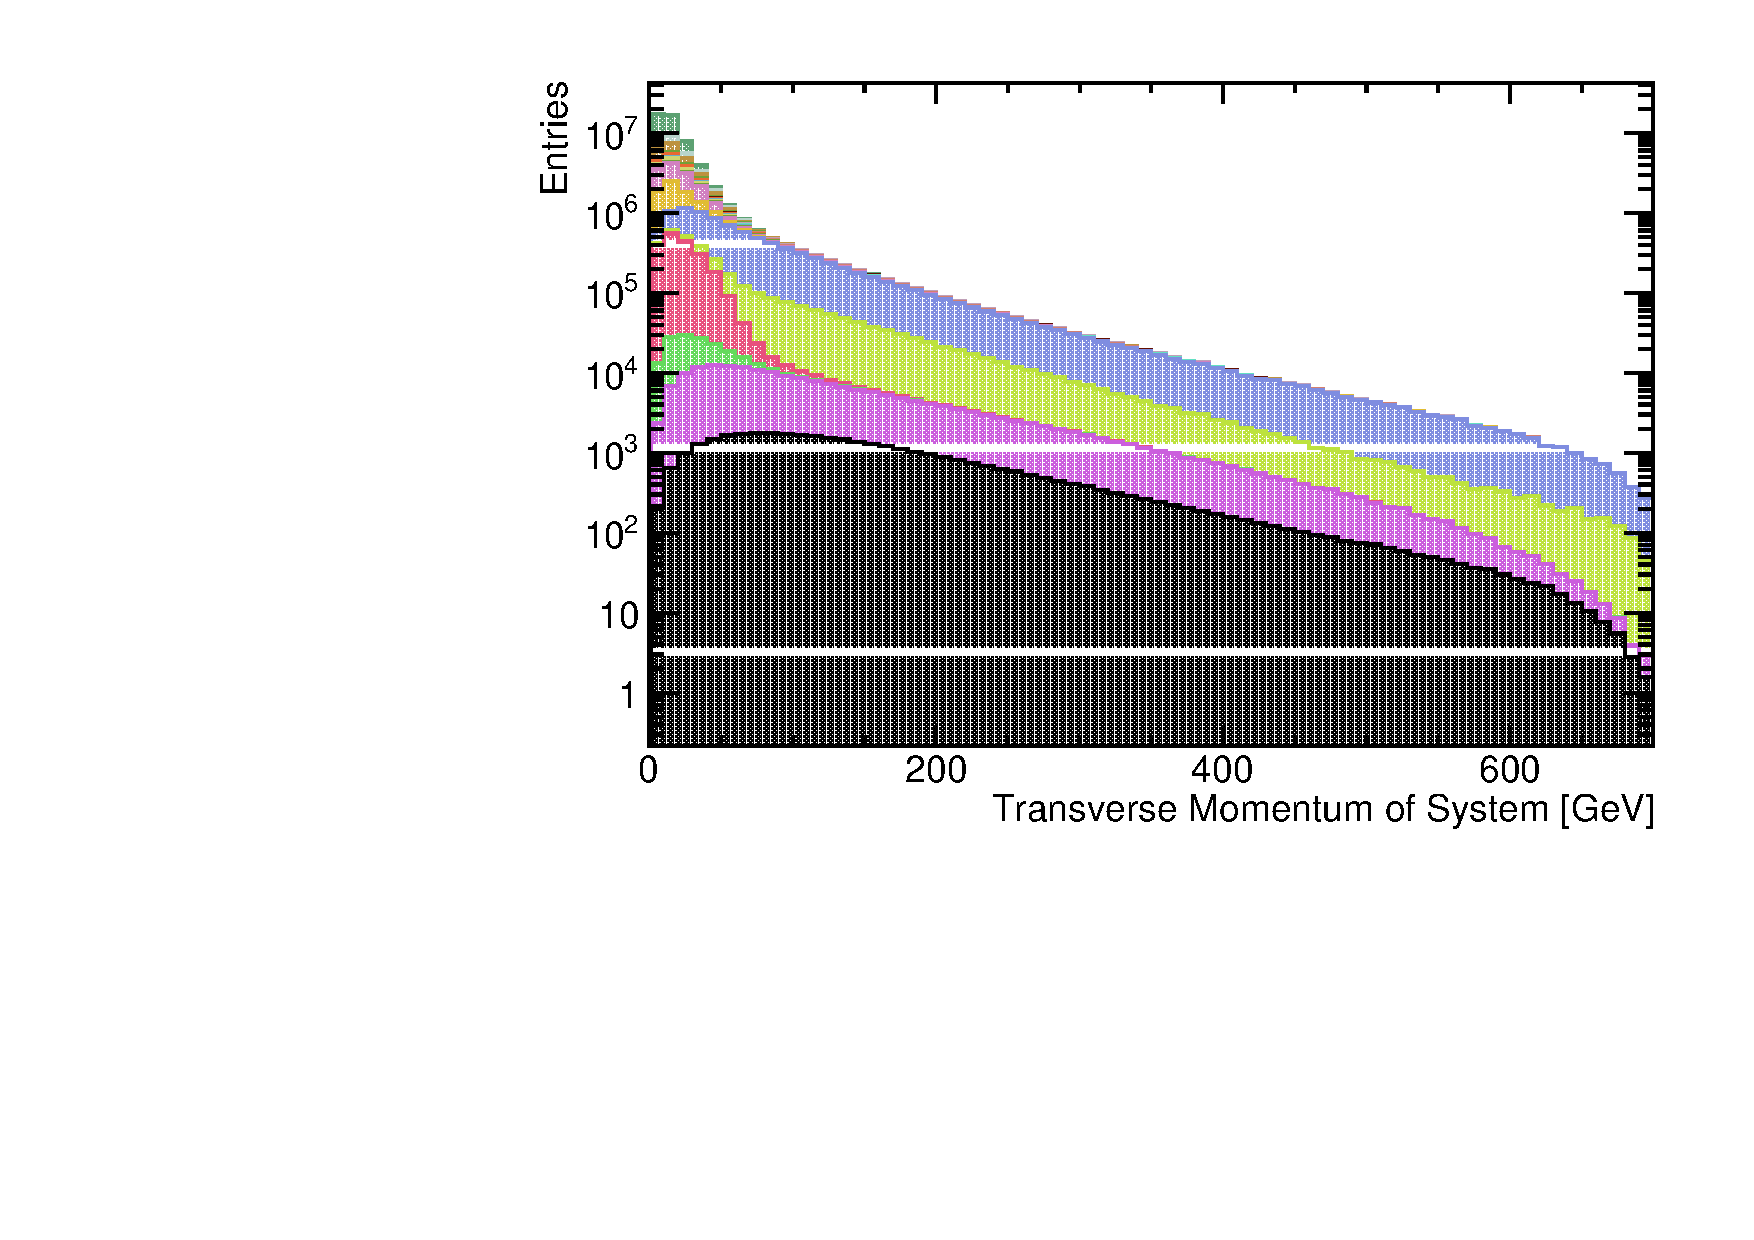
\includegraphics[width=0.5\textwidth]{PhysicsAnalysis/Plots/PreSelection/1400GeV/TransverseMomentum.pdf}}
\subfloat[]{\label{fig:preselection1400_2}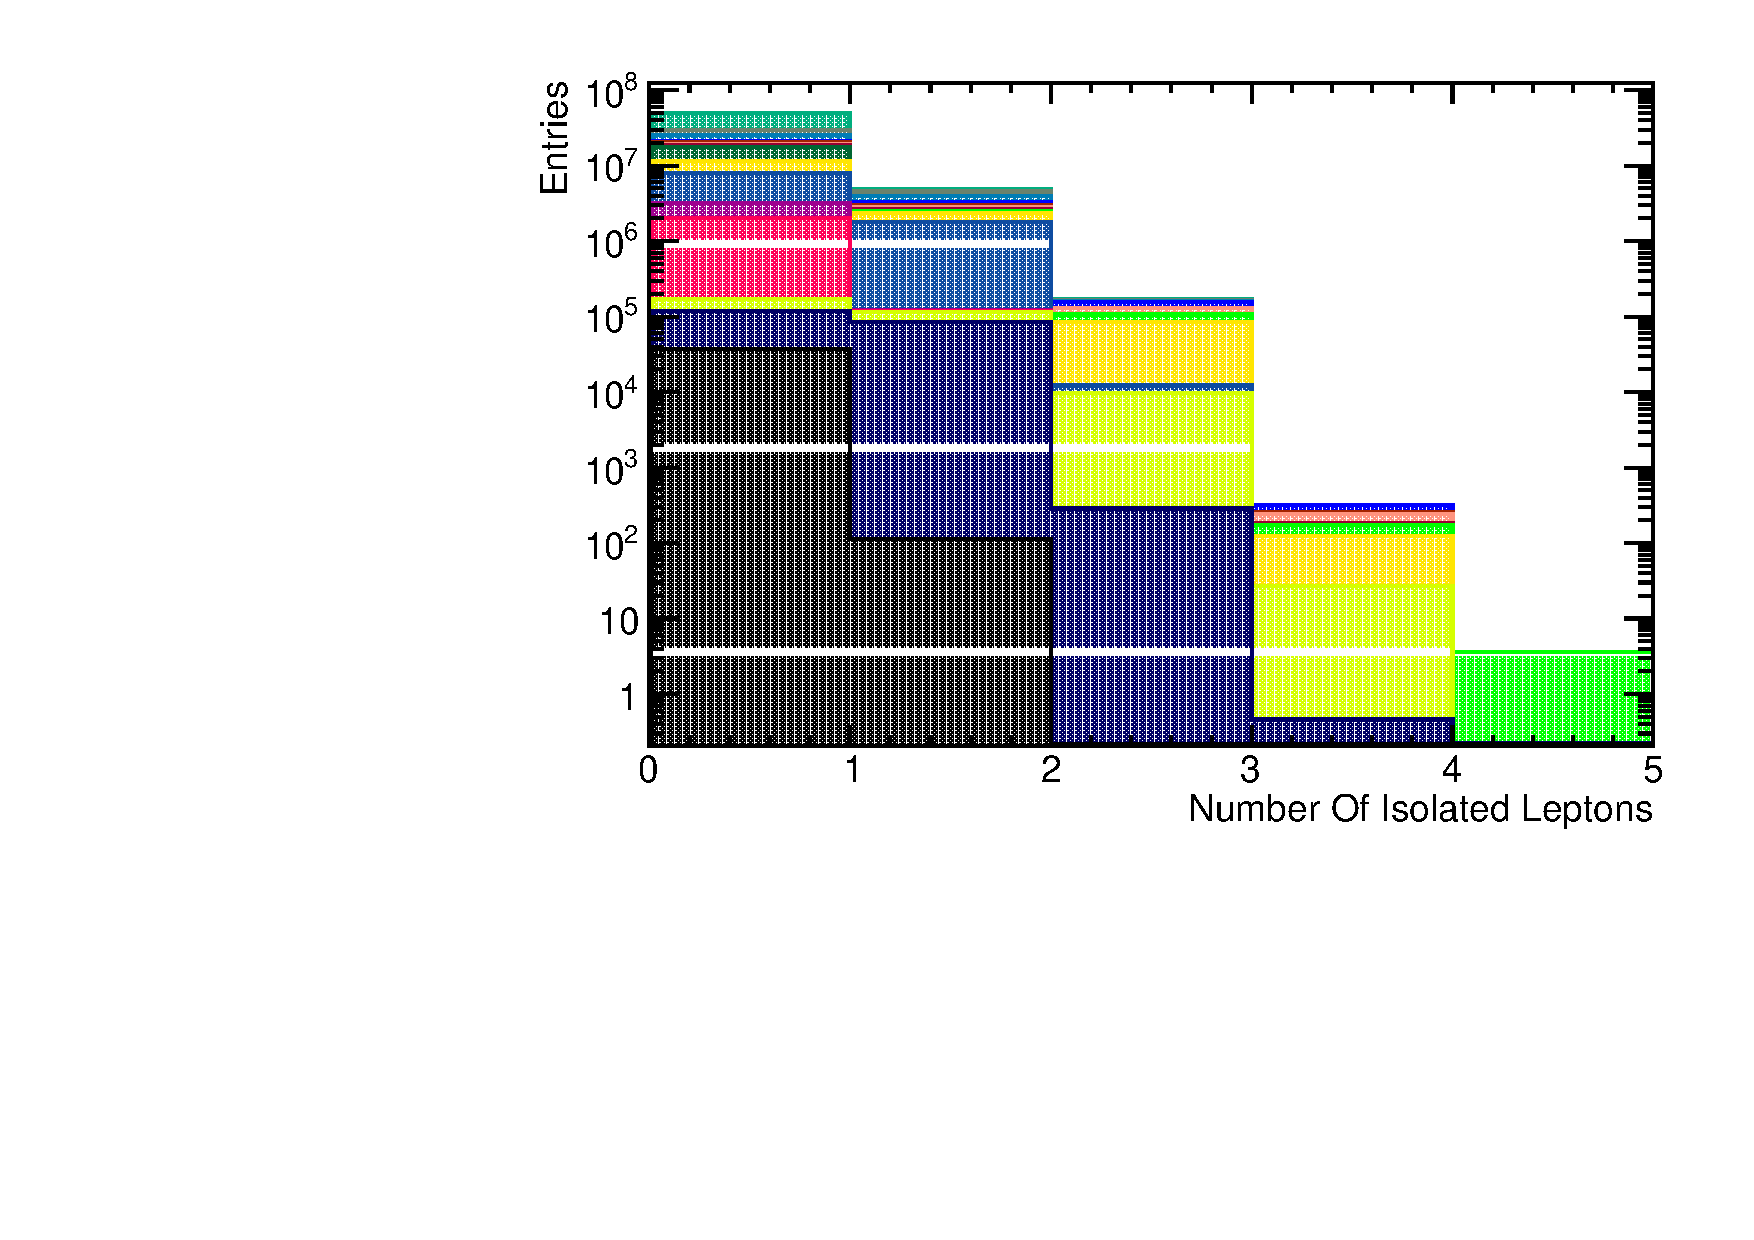
\includegraphics[width=0.5\textwidth]{PhysicsAnalysis/Plots/PreSelection/1400GeV/NumberOfIsolatedLeptons.pdf}} \hfill
\subfloat[]{\label{fig:preselection1400_3}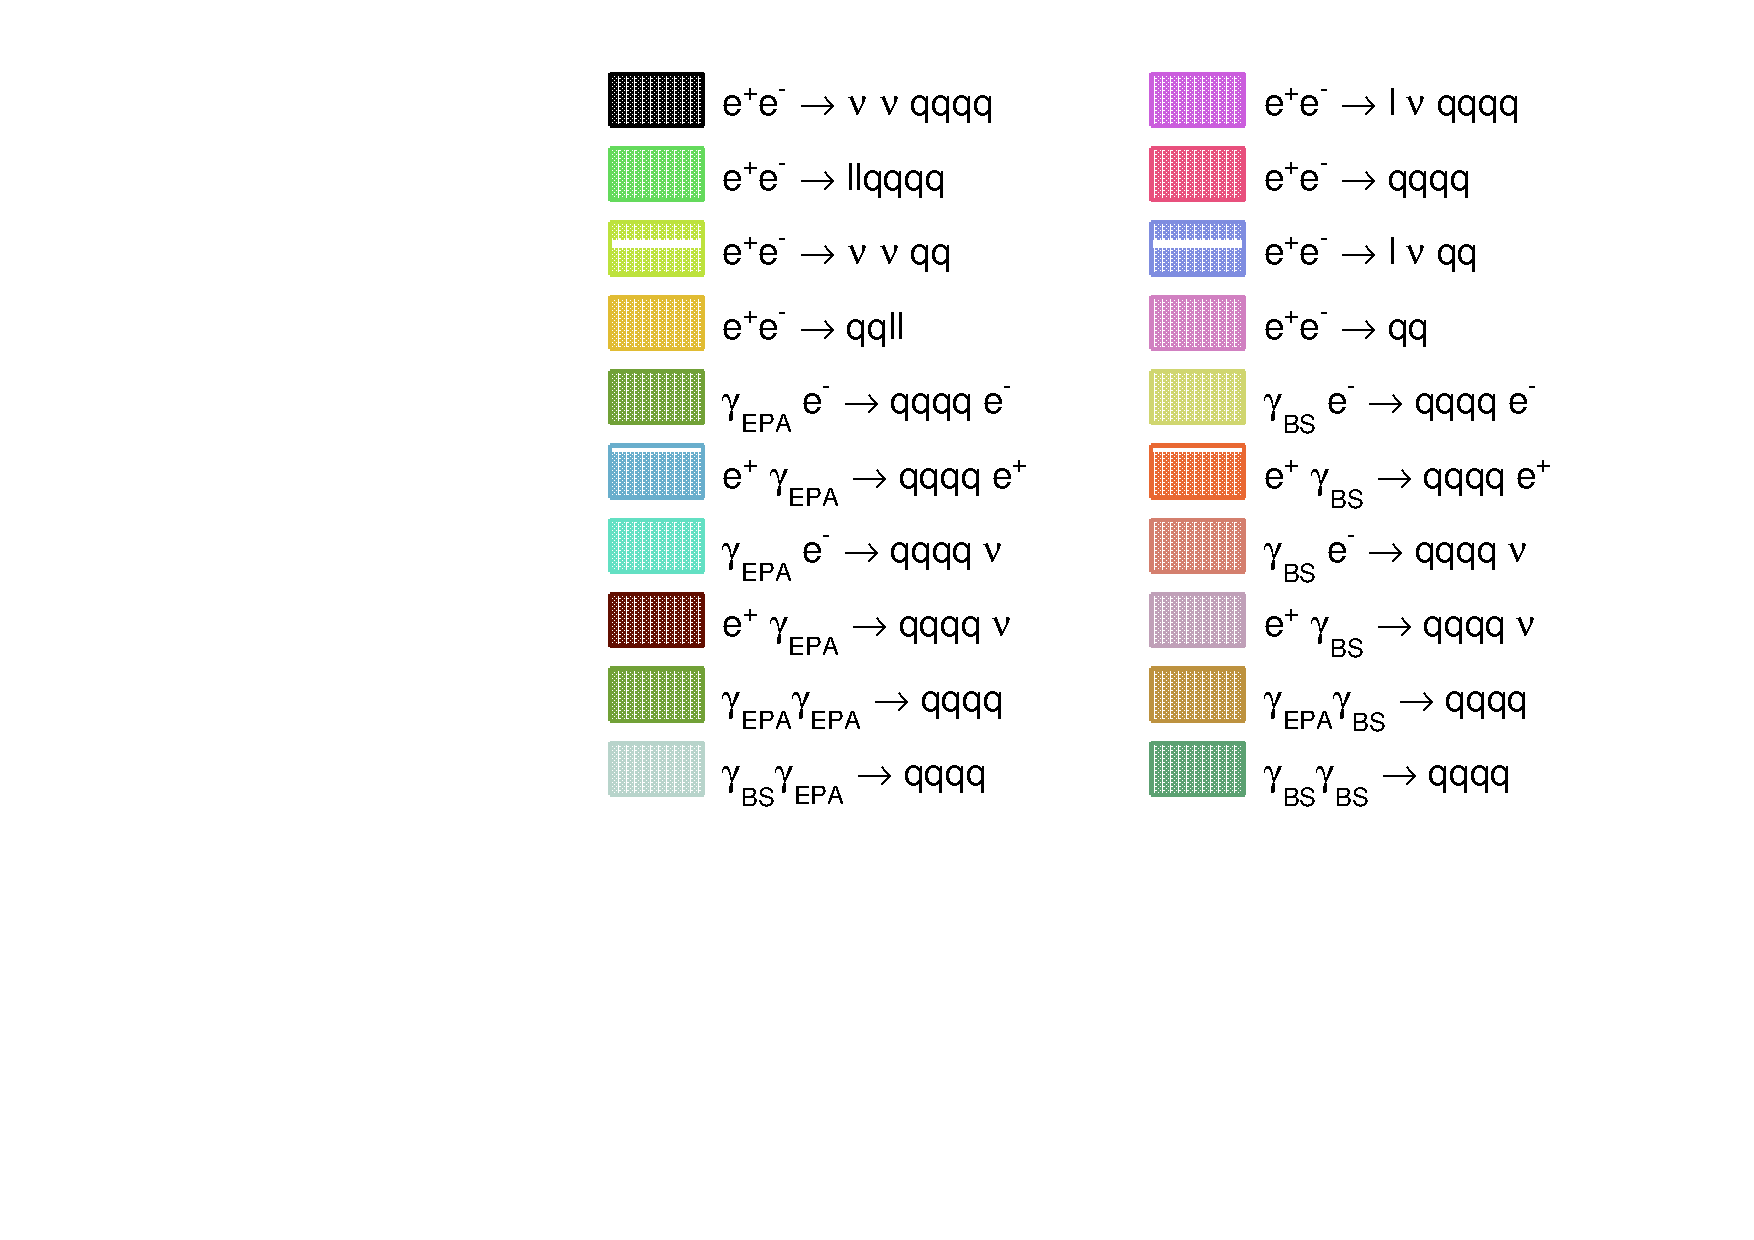
\includegraphics[width=0.5\textwidth]{PhysicsAnalysis/Plots/PreSelection/1400GeV/Legend.pdf}}
\caption[Distribution of variables cut on in the preselection at 1.4~TeV.  \protect\subref{fig:preselection1400_1} The transverse momentum of the visible system.  \protect\subref{fig:preselection1400_2} The number of isolated leptons in the system.  \protect\subref{fig:preselection1400_3} The legend for the preceding plots.]{Distribution of variables cut on in the preselection at 1.4~TeV.  \protect\subref{fig:preselection1400_1} The transverse momentum of the visible system.  \protect\subref{fig:preselection1400_2} The number of isolated leptons in the system.  \protect\subref{fig:preselection1400_3} The legend for the preceding plots.}
\label{fig:preselection1400}
\end{figure}

%========================================================================================

\subsection{Multivariate analysis}
\label{sec:mva1400GeV}
Having established the preselection cuts a MVA was applied, using the TMVA toolkit \cite{Hocker:2007ht}, to refine the event selection.  The signal and background final state samples were halved; one half sample was used to train the MVA and the remaining half sample was used in the subsequent analysis.  The sample sizes for the signal and backgrounds were sufficiently large that halving them in this way had a negligible impact on the subsequent analysis.  The following variables were used for training of the MVA:
\begin{itemize}
\item Number of PFOs in each jet. 
\item Energy of the highest energy PFO.
\item Energy of the highest energy electron.
\item Cosine of the polar angle of the highest energy track.
\item Energy of the candidate bosons.
\item Invariant mass of the candidate bosons.
\item Acolinearity of the candidate boson pair.
\item The vector sum of the transverse momentum of all PFOs in the event. 
\item Sphericity. 
\item Jet clustering parameter variables, $y_{ij}$ where $i = 3,4$ and $j=i+1$.  The variable used in the multivariate analysis is $-\text{log}_{10}(y_{ij})$.
\end{itemize}

A variety of MVA options were considered and it was found that the optimal algorithm was the boosted decision tree (BDT) as shown by figure \ref{fig:mvaalternatives1400GeV}.  

\begin{figure}
\centering
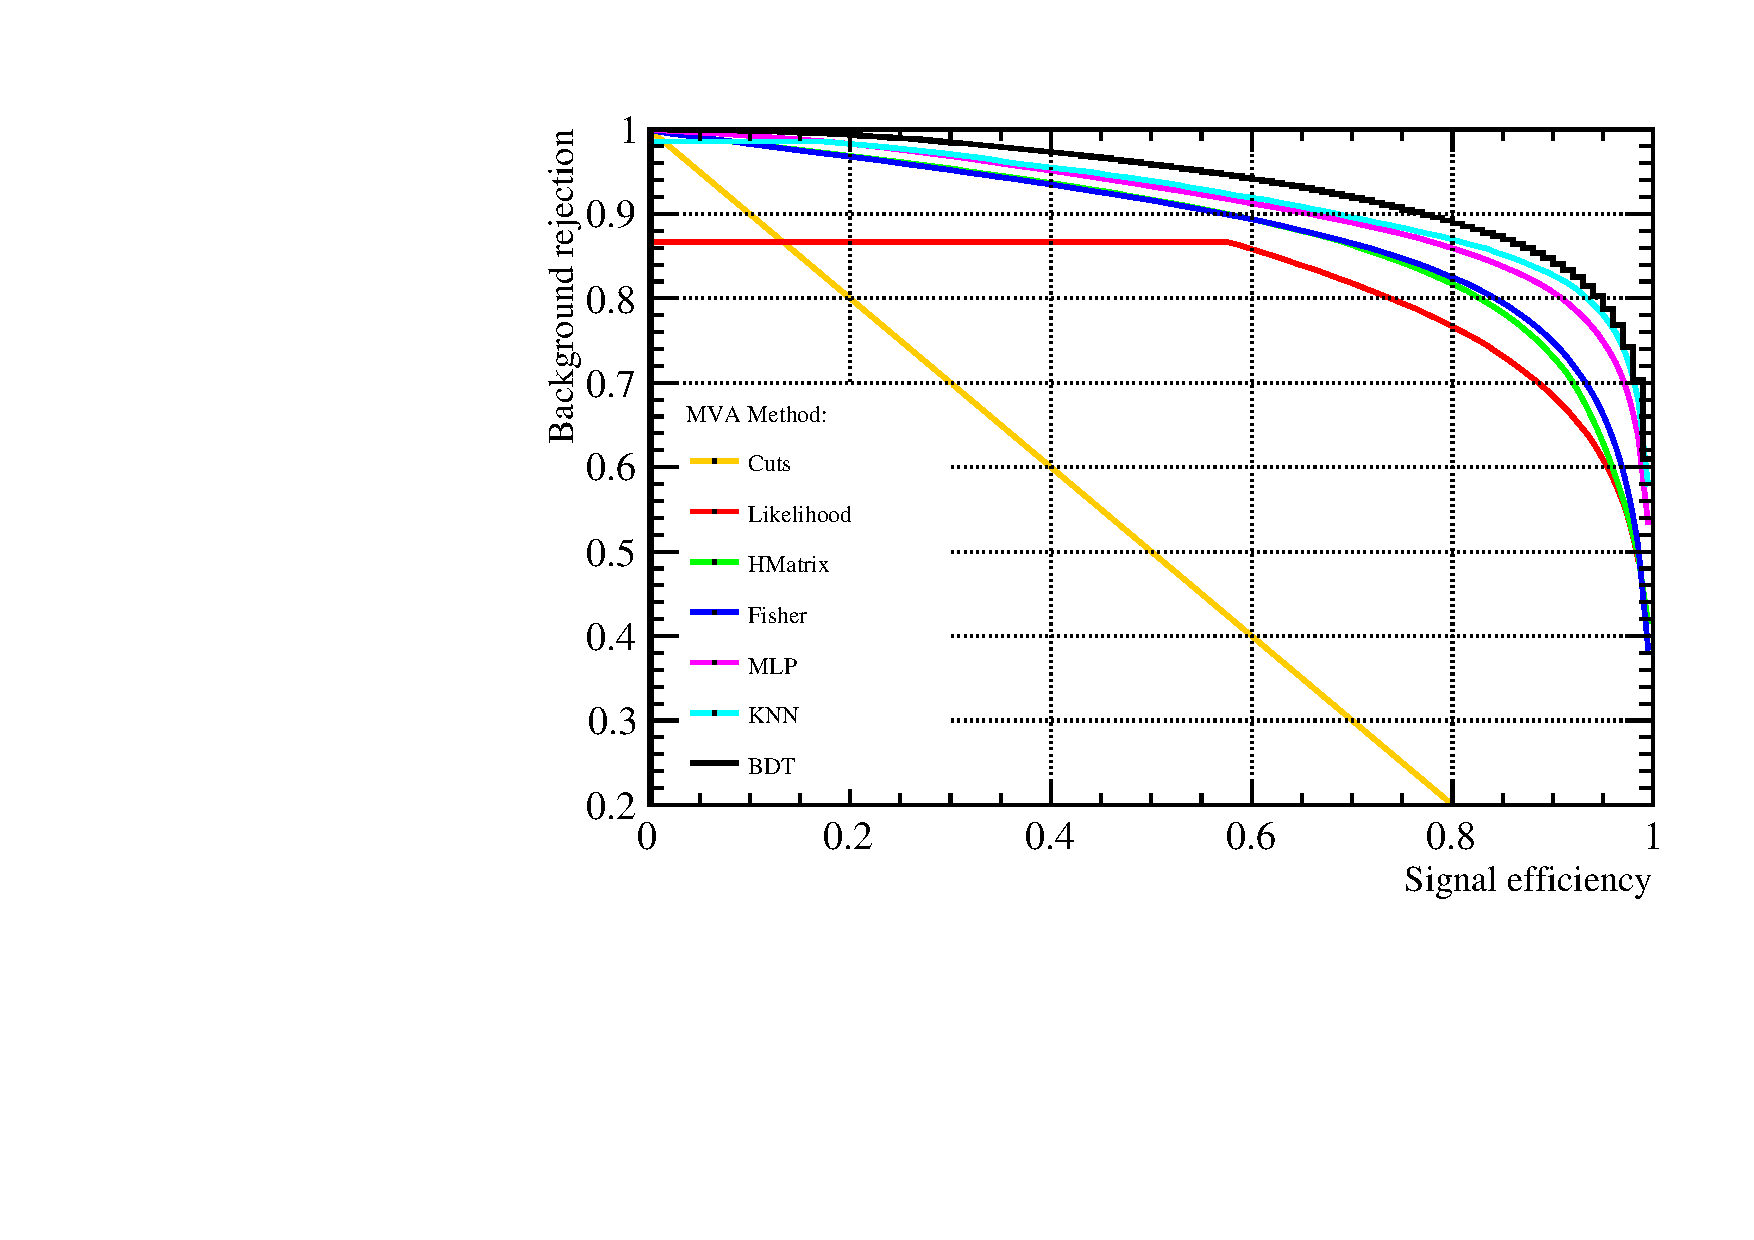
\includegraphics[width=0.75\textwidth]{PhysicsAnalysis/Plots/MVAPlots/1400GeV/ThesisPlotMVAAlternatives1400GeV.pdf}
\caption[Background rejection as a function of signal efficiency for a variety of MVA options at 1.4~TeV.]{Background rejection as a function of signal efficiency for a variety of MVA options at 1.4~TeV.} 
\label{fig:mvaalternatives1400GeV}
\end{figure}

The BDT was further optimised by varying the number of trees used, the depth of the trees and the number of cuts applied and an optimal significance, S/$\sqrt(\text{S + B})$, of 52.7 was obtained.  In the determination of the significance S (B) is the number of signal (background) events passing the preselection.

%========================================================================================

\subsection{Event Selection Summary}
\label{sec:eventselsummary1400GeV}
The event selection is summarised using the distribution of the invariant mass of the candidate bosons, which for the signal final state should peak around the W mass.  This distribution is shown in figure \ref{fig:synbosonmass1400GeVMVAimpact} with no event selection, with the preselection cuts applied and with both preselections cuts and MVA applied.  The event selection is also summarised using efficiencies shown in table \ref{table:selectionsummary1400GeV}.

As expected the dominant background processes after the MVA is applied are those that will look identical to the signal process, i.e. qqqq with missing energy.  Two smaller sources of background are also present: two jet events with missing energy that are confused with four jet events with missing energy and events where a lepton is not properly reconstructed causing the event to look like four jets and missing energy.  

\begin{figure}
\centering
\subfloat[]{\label{fig:nocutssynbosonmass1400GeVMVAimpact}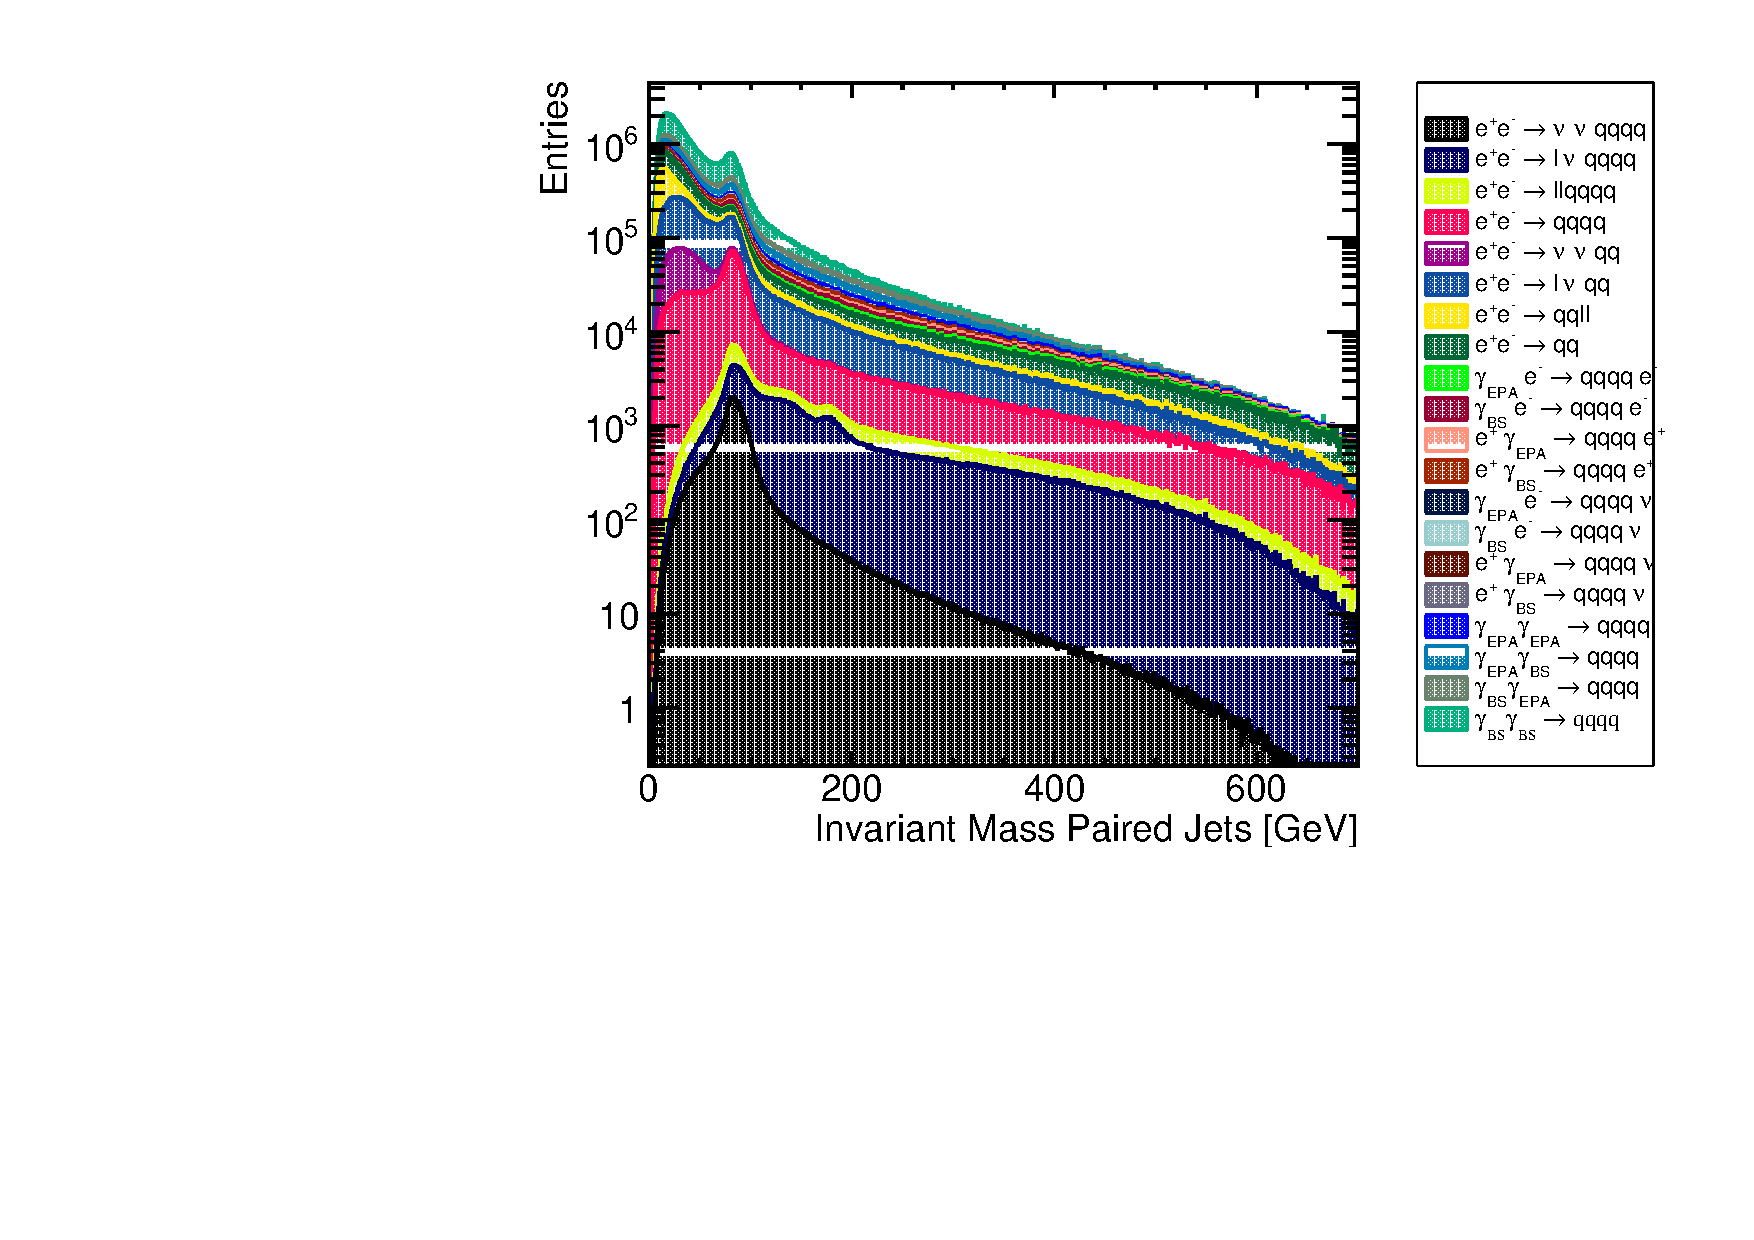
\includegraphics[width=0.5\textwidth]{PhysicsAnalysis/Plots/PostMVASelection/1400GeV/InvariantMassSynBosons_1400GeV_No_Cuts_StackPlot.pdf}}
\subfloat[]{\label{fig:nocutssynbosonmass1400GeVMVAimpact}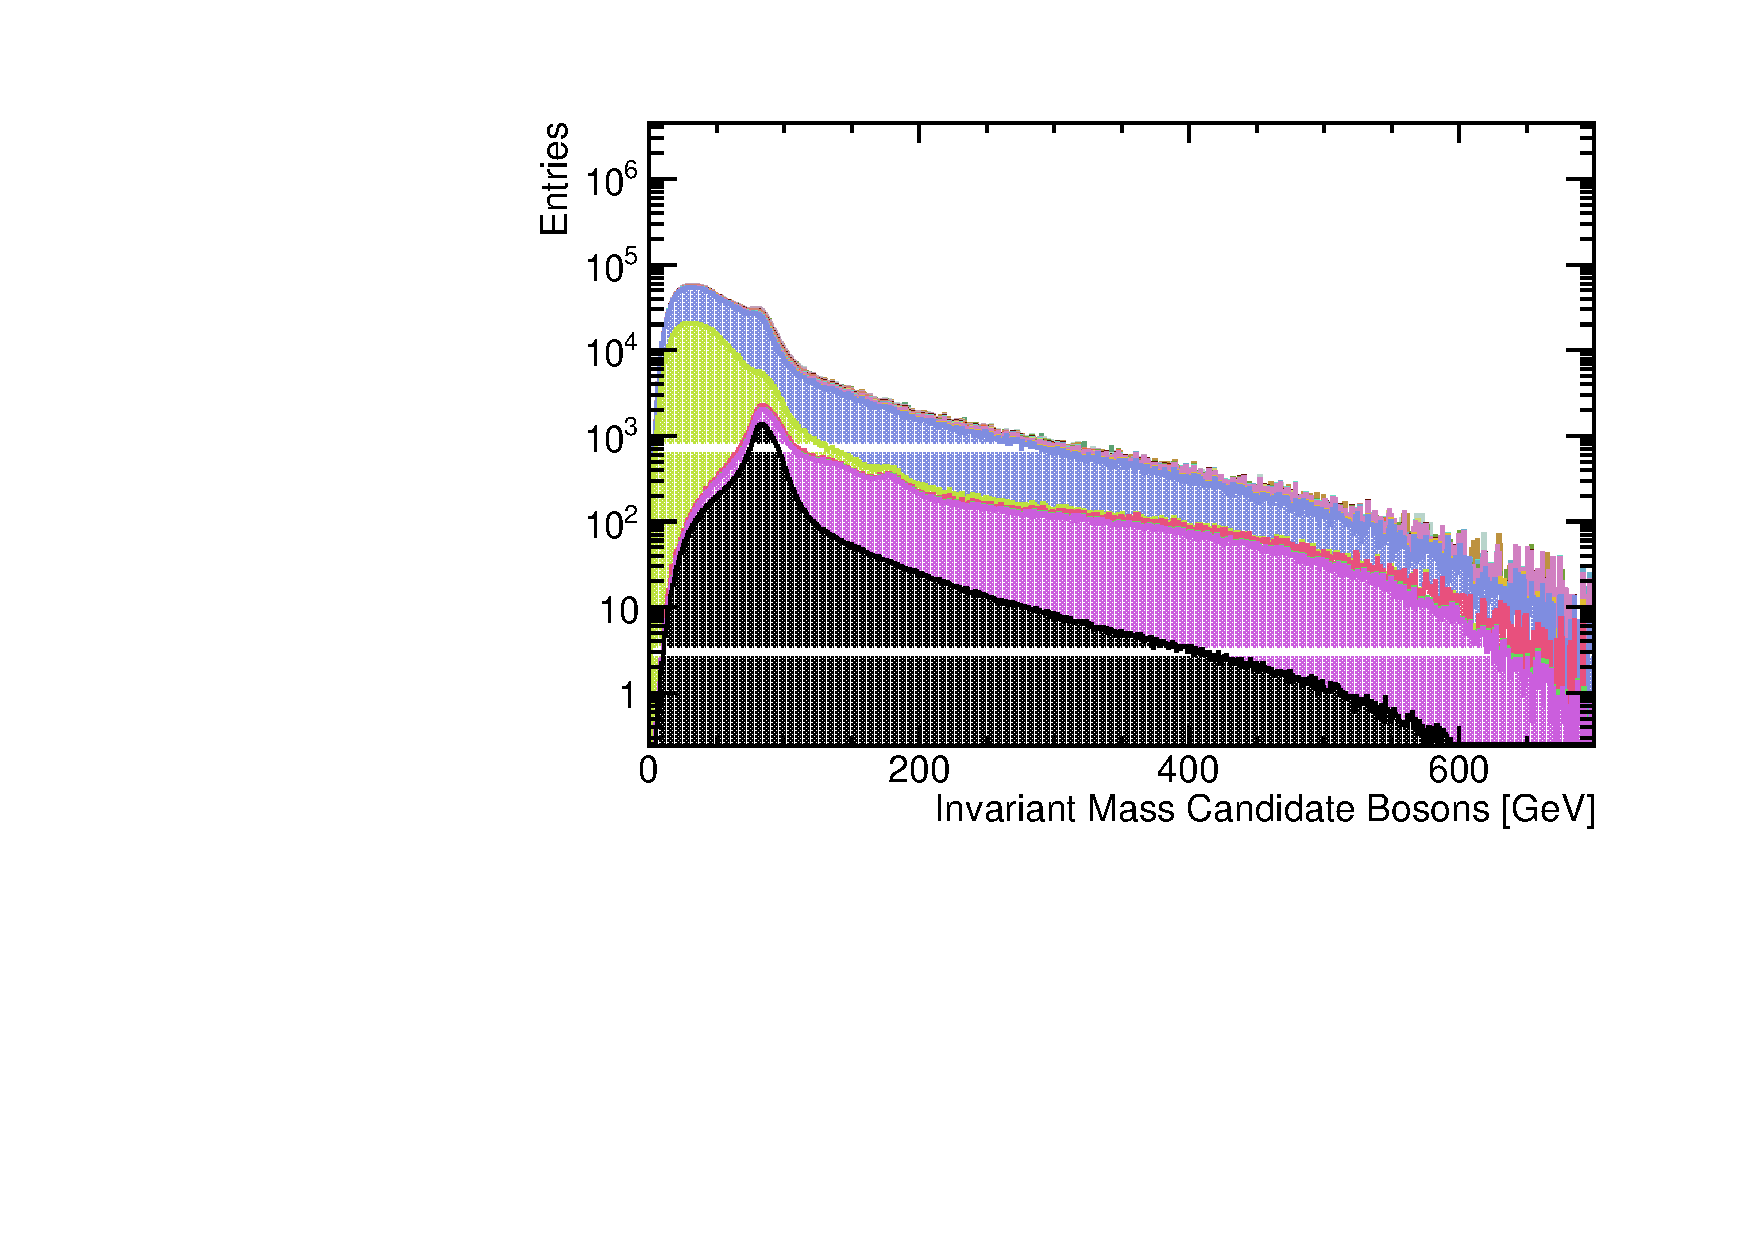
\includegraphics[width=0.5\textwidth]{PhysicsAnalysis/Plots/PostMVASelection/1400GeV/InvariantMassSynBosons_1400GeV_Pt_gt100GeV_NIsoLep_eq0_Cuts_StackPlot.pdf}}\hfill
\subfloat[]{\label{fig:postmvasynbosonmass1400GeVMVAimpact}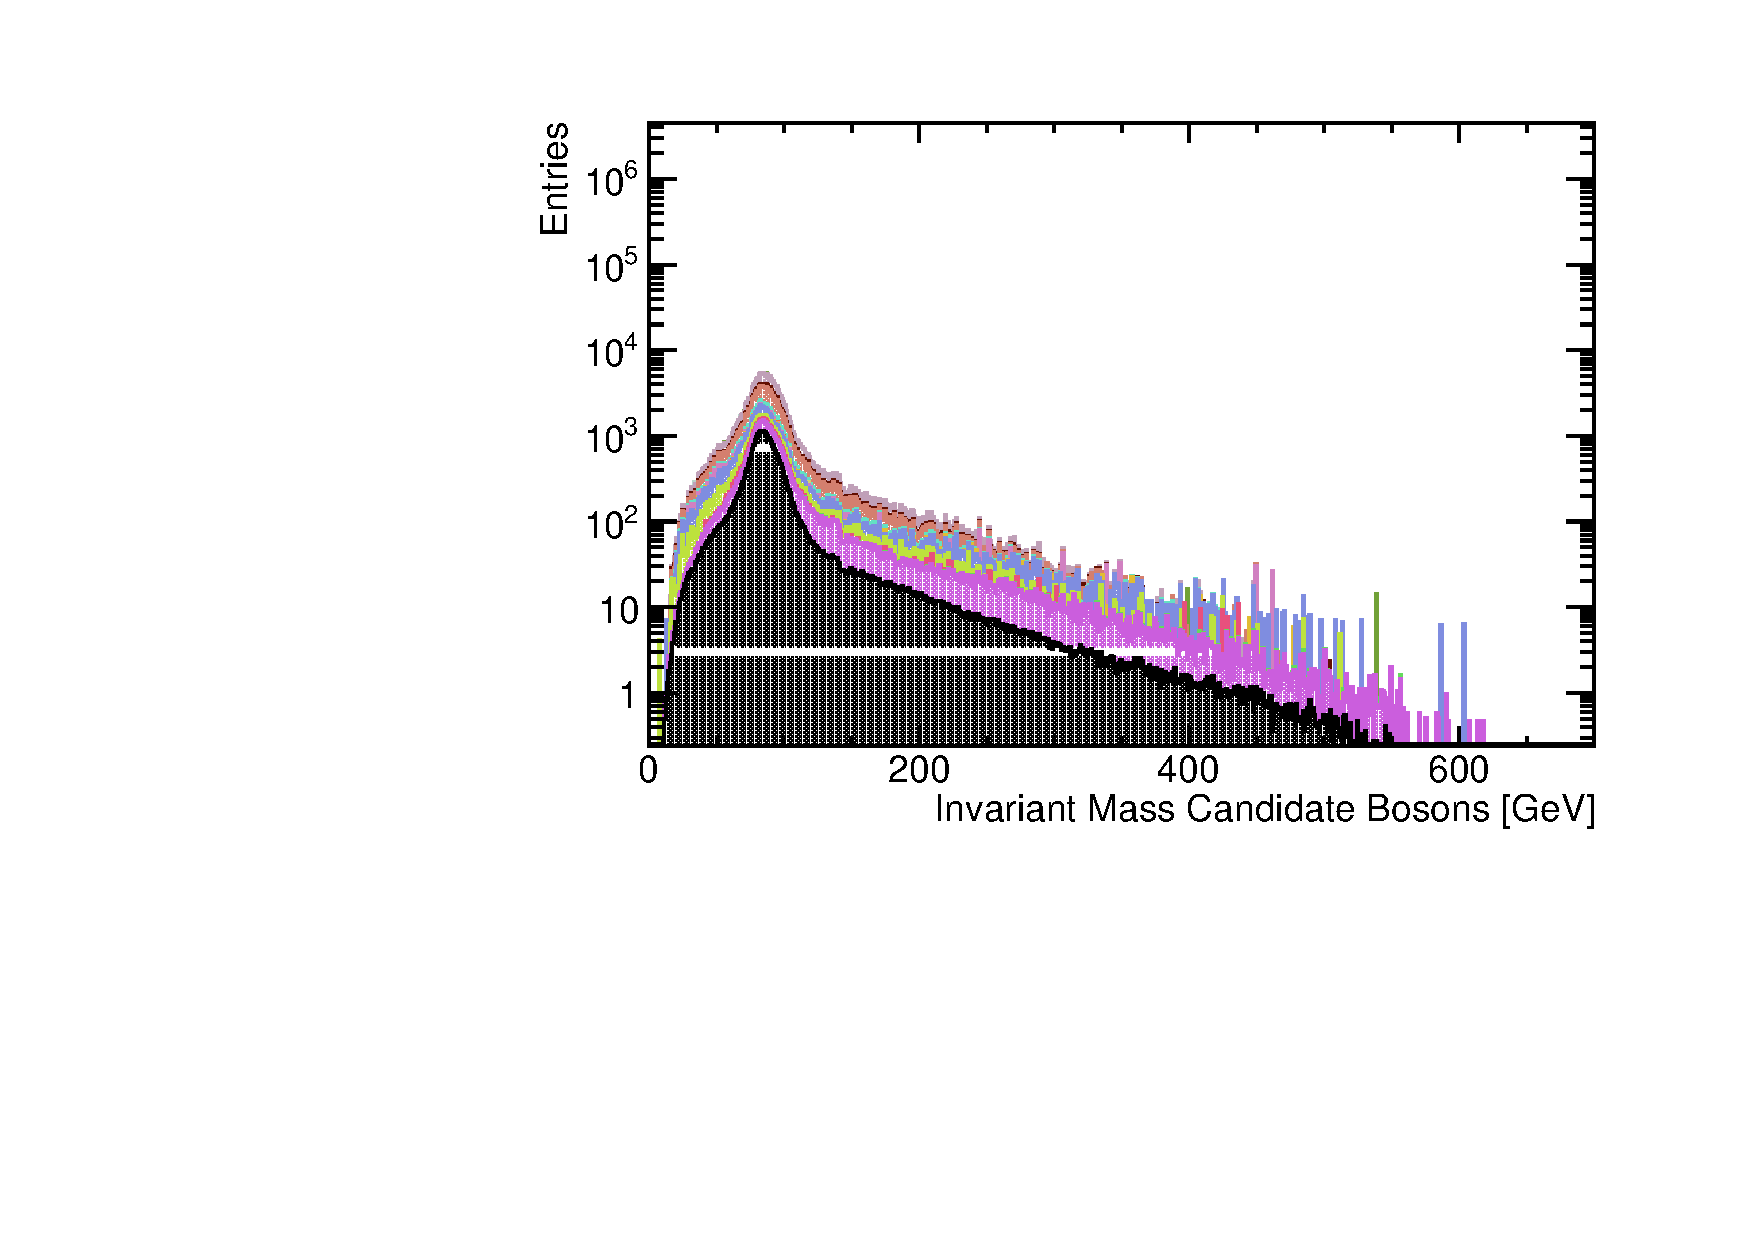
\includegraphics[width=0.5\textwidth]{PhysicsAnalysis/Plots/PostMVASelection/1400GeV/InvariantMassSynBosons_1400GeV_PostPreSelection_PostMVA_Cuts_StackPlot.pdf}} 
\subfloat[]{\label{fig:legendselection}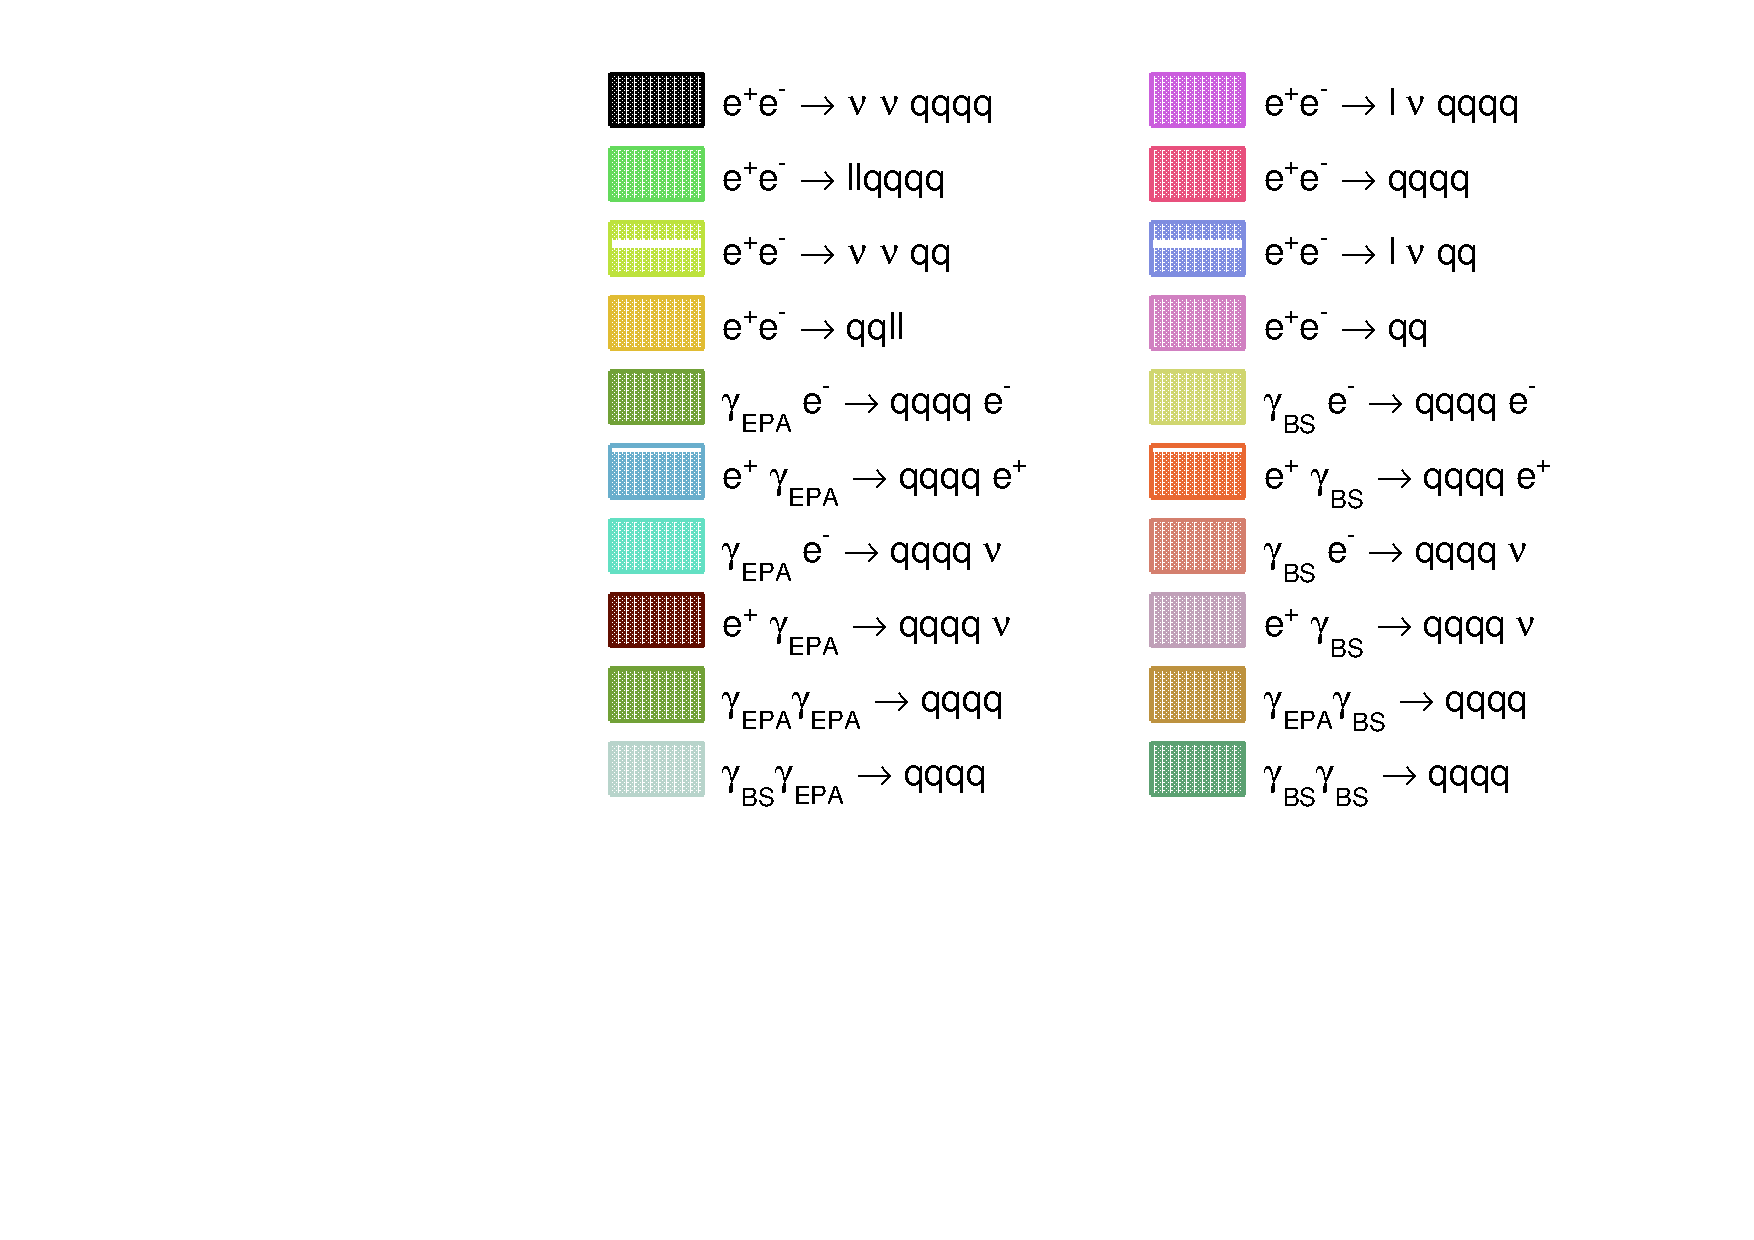
\includegraphics[width=0.5\textwidth]{PhysicsAnalysis/Plots/PreSelection/1400GeV/Legend.pdf}}
\caption[Impact of preselection and MVA on the reconstructed invariant mass of the bosons arising from jet pairing at 1.4~TeV.   \protect\subref{fig:nocutssynbosonmass1400GeVMVAimpact} No cuts applied.  \protect\subref{fig:nocutssynbosonmass1400GeVMVAimpact} Preselection cuts applied.  \protect\subref{fig:postmvasynbosonmass1400GeVMVAimpact} MVA with preselection applied.  \protect\subref{fig:legendselection} The legend for the event selection plots.]{Impact of preselection and MVA on the reconstructed invariant mass of the bosons arising from jet pairing at 1.4~TeV.   \protect\subref{fig:nocutssynbosonmass1400GeVMVAimpact} No cuts applied.  \protect\subref{fig:nocutssynbosonmass1400GeVMVAimpact} Preselection cuts applied.  \protect\subref{fig:postmvasynbosonmass1400GeVMVAimpact} MVA with preselection applied.  \protect\subref{fig:legendselection} The legend for the event selection plots.}
\label{fig:synbosonmass1400GeVMVAimpact}
\end{figure}

\begin{table}[h!]
\centering
\begin{tabular}{ l r r r }
\hline
Final State & $\epsilon_{\text{presel}}$ & $\epsilon_{\text{BDT}}$ & $N_{\text{BDT}}$ \\ 
\hline
$\text{e}^{+}\text{e}^{-} \rightarrow \nu{\nu}\text{qqqq}$ & 64.1\% & 44.5\% & 16,470 \\
$\text{e}^{+}\text{e}^{-} \rightarrow \text{l}\nu\text{qqqq}$ & 26.1\% & 5.2\% & 8,582 \\
$\text{e}^{+}\text{e}^{-} \rightarrow \text{llqqqq}$ & 0.8\% & 0.1\% & 100 \\
$\text{e}^{+}\text{e}^{-} \rightarrow \text{qqqq}$ & 0.3\% & 0.1\% & 1,698 \\
$\text{e}^{+}\text{e}^{-} \rightarrow \nu{\nu}\text{qq}$ & 43.4\% & 0.5\% & 5,351 \\
$\text{e}^{+}\text{e}^{-} \rightarrow \text{l}\nu\text{qq}$ & 19.1\% & 0.1\% & 9,319 \\
$\text{e}^{+}\text{e}^{-} \rightarrow \text{llqq}$ & 0.1\% & - & 234 \\
$\text{e}^{+}\text{e}^{-} \rightarrow \text{qq}$ & 0.6\% & - & 1,586 \\
$\gamma_{\text{EPA}}\text{e}^{-} \rightarrow \text{qqqq}\text{e}^{-}$ & 0.2\% & - & 48 \\
$\gamma_{\text{BS}}\text{e}^{-} \rightarrow \text{qqqq}\text{e}^{-}$ & 0.1\% & - & 42 \\
$\text{e}^{+}\gamma_{\text{EPA}} \rightarrow \text{qqqq}\text{e}^{+}$ & 0.3\% & - & 19 \\
$\text{e}^{+}\gamma_{\text{BS}} \rightarrow \text{qqqq}\text{e}^{+}$ & - & - & 65 \\
$\gamma_{\text{EPA}}\text{e}^{-} \rightarrow \text{qqqq}\nu$ & 26.0\% & 9.0\% & 4,421 \\
$\gamma_{\text{BS}}\text{e}^{-} \rightarrow \text{qqqq}\nu$ & 36.1\% & 15.0\% & 23,150 \\
$\text{e}^{+}\gamma_{\text{EPA}} \rightarrow \text{qqqq}\nu$ & 25.9\% & 9.2\% & 4,495 \\
$\text{e}^{+}\gamma_{\text{BS}} \rightarrow \text{qqqq}\nu$ & 36.4\% & 15.3\% & 23,410 \\
$\gamma_{\text{EPA}}\gamma_{\text{EPA}} \rightarrow \text{qqqq}$ & 0.2\% & - & 81 \\
$\gamma_{\text{EPA}}\gamma_{\text{BS}} \rightarrow \text{qqqq}$ & 0.1\% & - & 55 \\
$\gamma_{\text{BS}}\gamma_{\text{EPA}} \rightarrow \text{qqqq}$ & - & - & 53 \\
$\gamma_{\text{BS}}\gamma_{\text{BS}} \rightarrow \text{qqqq}$ & - & - & 0 \\
\hline
\end{tabular}
\caption[Selection summary at 1.4~TeV.   The EPA and BS subscript on the incoming photon indicates whether the photon is generated from the equivalent photon approximation or beamstrahlung.  Cells omitting the efficiency indicate an efficiency of less than 0.1\%.]{Selection summary at 1.4~TeV.   The EPA and BS subscript on the incoming photon indicates whether the photon is generated from the equivalent photon approximation or beamstrahlung.  Cells omitting the efficiency indicate an efficiency of less than 0.1\%.}
\label{table:selectionsummary1400GeV}
\end{table}

%========================================================================================
%========================================================================================

\section{Effect of Anomalous Coupling/Fitting Methodology}
\label{sec:fitting}
This section describes the procedure used for constructing the $\chi^{2}$ surface and the subsequent confidence contours used to determine the sensitivity of CLIC to the anomalous gauge couplings $\alpha_{4}$ and $\alpha_{5}$.

%========================================================================================

\subsection{Sensitive Distribution}
The sensitivity of CLIC to the anomalous gauge couplings is determined through the use of a $\chi^{2}$ fit to the distribution of $M_{VV}$, the invariant mass of the visible system.  For a given event, the jet clustering and pairing proceeds as described in section \ref{sec:analysis}.  This leads to each event being clustered into four jets that are then paired up to give two candidate bosons.  The distribution of $M_{VV}$ proved to be highly sensitive to the anomalous gauge couplings, particularly for at large invariant masses, as shown in figure \ref{fig:mvv}.

Two other distributions were considered for this sensitivity study, but proved to be less sensitive than $M_{VV}$: $\text{cos}\theta^{*}_{Jets}$, the angle between the boost direction and the back to back quark jets in the rest frame of the candidate bosons, and $\text{cos}\theta^{*}_{Bosons}$, the angle between the boost direction and the back to back candidate bosons in the rest frame of the visible system.  The sensitivity of these variables can be seen in figure \ref{fig:costhetastar}.  It should be noted that there are two entries, one from each candidate boson, in the $\text{cos}\theta^{*}_{Jets}$ distribution per event.  To negate the effect of correlation between these two variables when performing the $\chi^{2}$ fit, a two dimensional fit of $\text{cos}\theta^{*}_{Jets}$ variable was applied where a distinction between candidate bosons was made based on their energy.  No such effect was present for the $\text{cos}\theta^{*}_{Bosons}$ variable as there is only a single pair of candidate bosons per event.

\begin{figure}[h!]
\centering
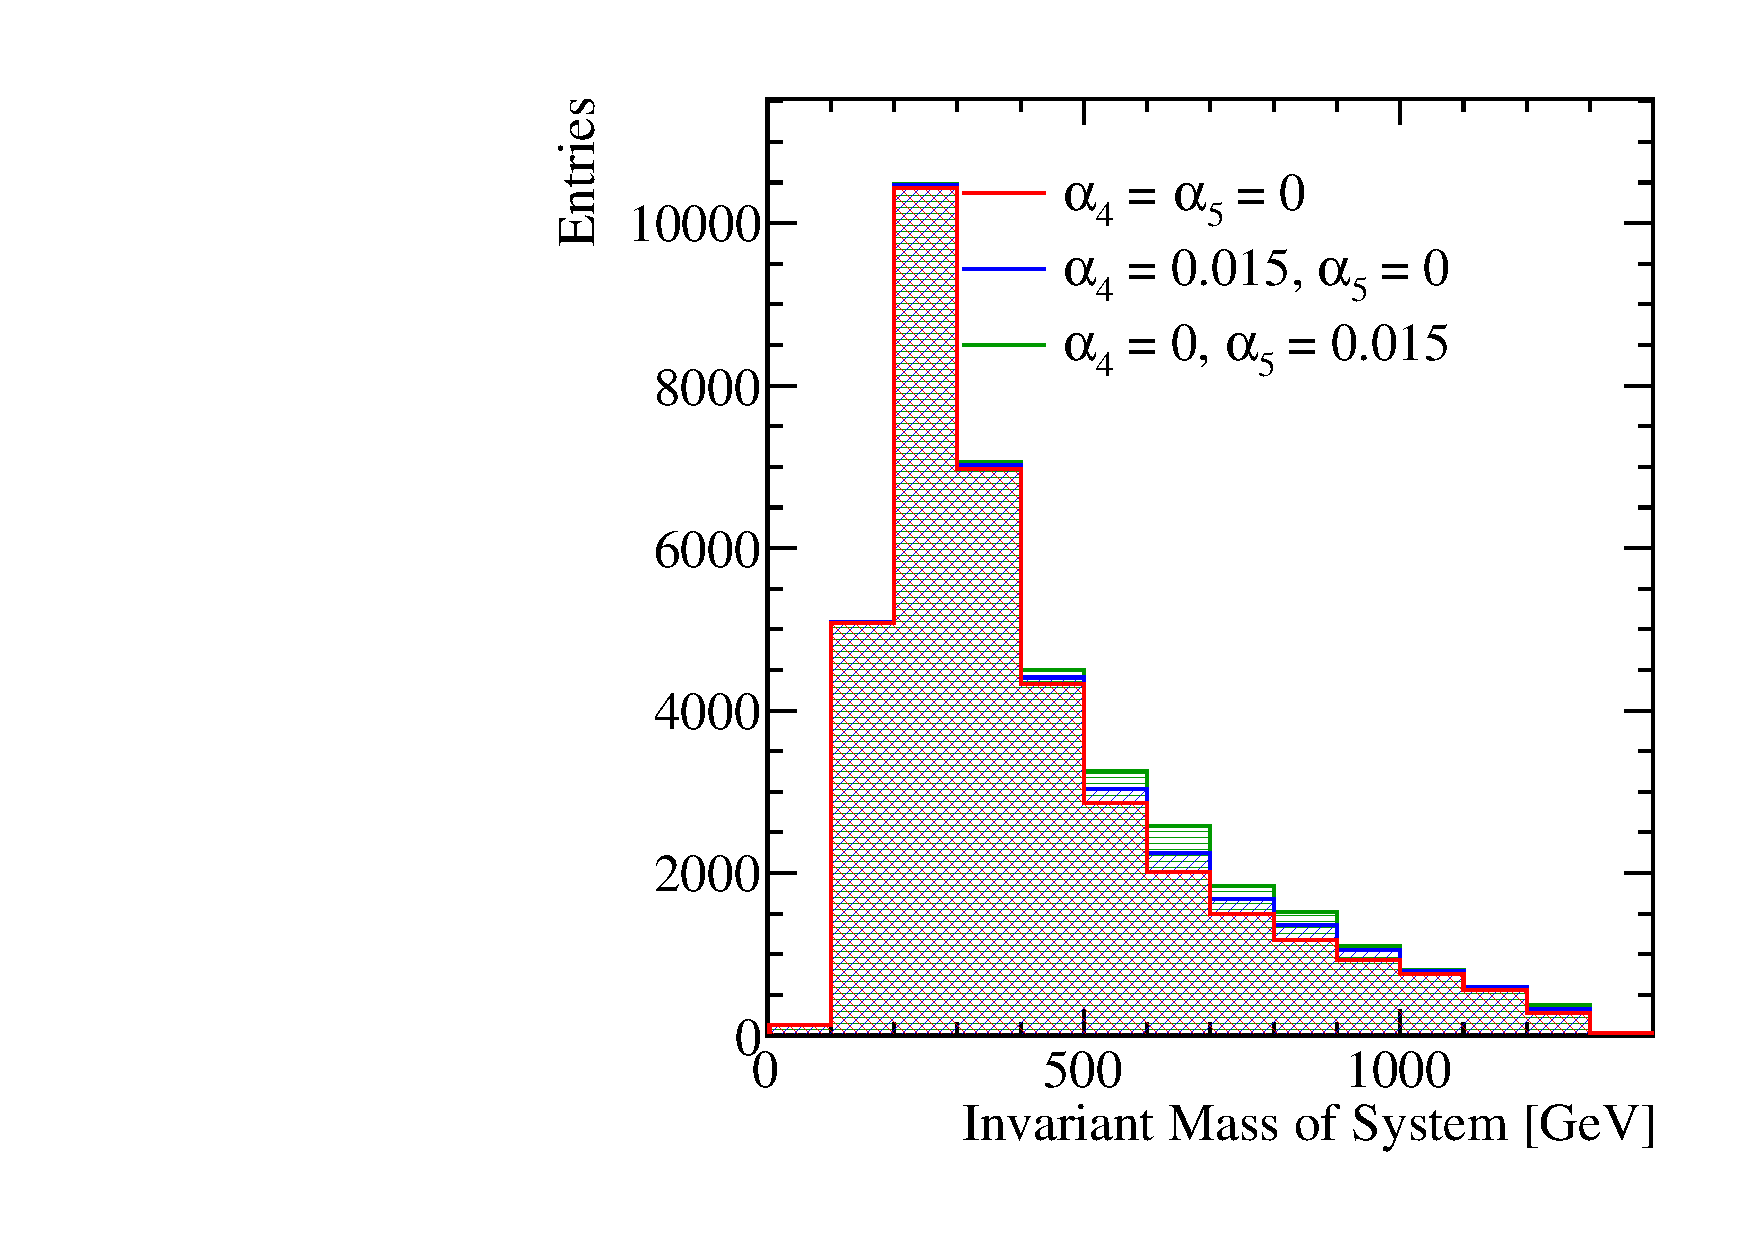
\includegraphics[width=0.5\textwidth]{PhysicsAnalysis/Plots/SensitiveDistributions/MVVs_SPFOs_kt_0p90_1400GeV.pdf}
\caption[The sensitivity of $M_{VV}$ to the anomalous gauge couplings $\alpha_{4}$ and $\alpha_{5}$ at 1.4~TeV.  The jet algorithm used was the longitudinally invariant kt algorithm with an R parameter of 0.9 and Selected PFOs were used.  This distribution is for the \nu{\nu}qqqq signal final state only.]{The sensitivity of $M_{VV}$ to the anomalous gauge couplings $\alpha_{4}$ and $\alpha_{5}$ at 1.4~TeV.  The jet algorithm used was the longitudinally invariant kt algorithm with an R parameter of 0.9 and Selected PFOs were used.  This distribution is for the \nu{\nu}qqqq signal final state only.}
\label{fig:mvv}
\end{figure}

\begin{figure}[h!]
\subfloat[]{\label{fig:costhetastarjets1400GeV} 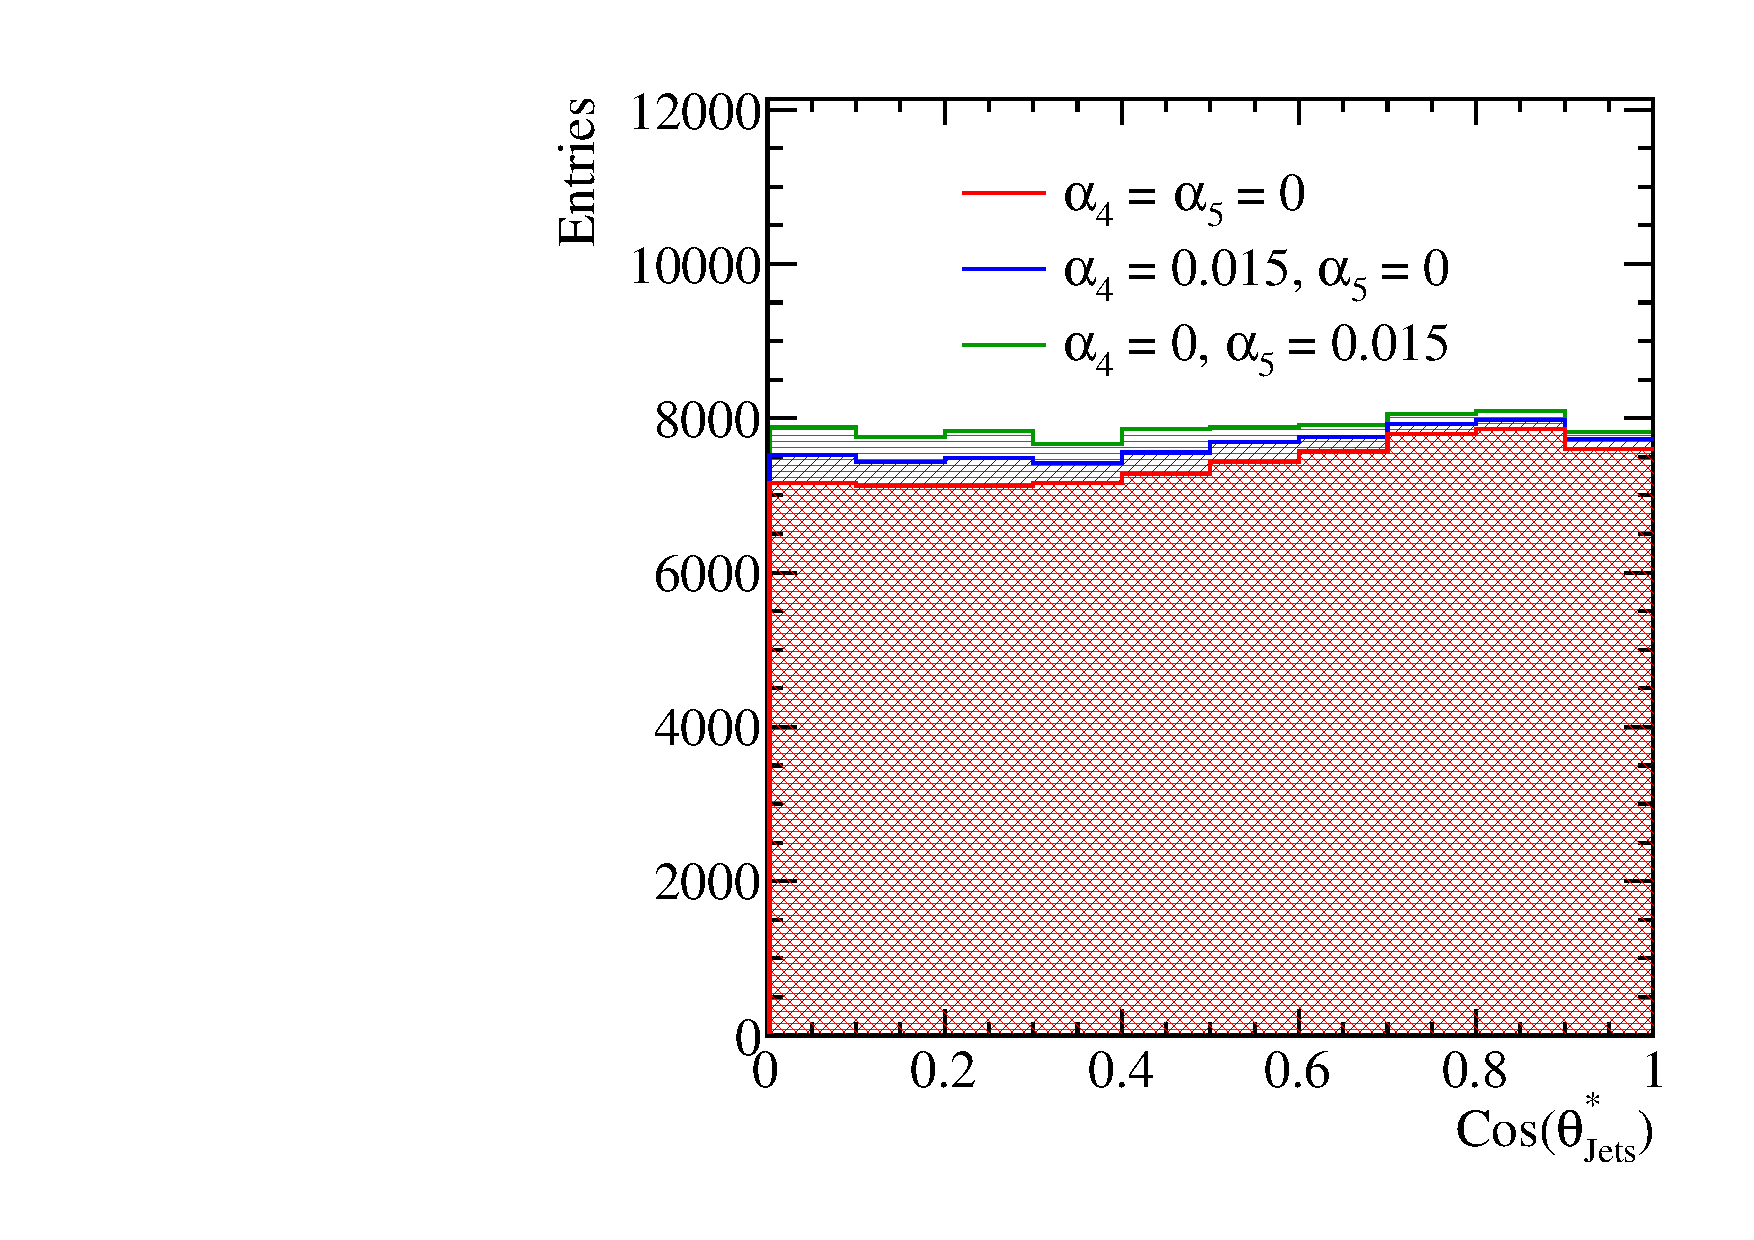
\includegraphics[width=0.5\textwidth]{PhysicsAnalysis/Plots/SensitiveDistributions/CosThetaStarSynJets_SPFOs_kt_0p90_1400GeV.pdf}}
\subfloat[]{\label{fig:costhetastarbosons1400GeV} 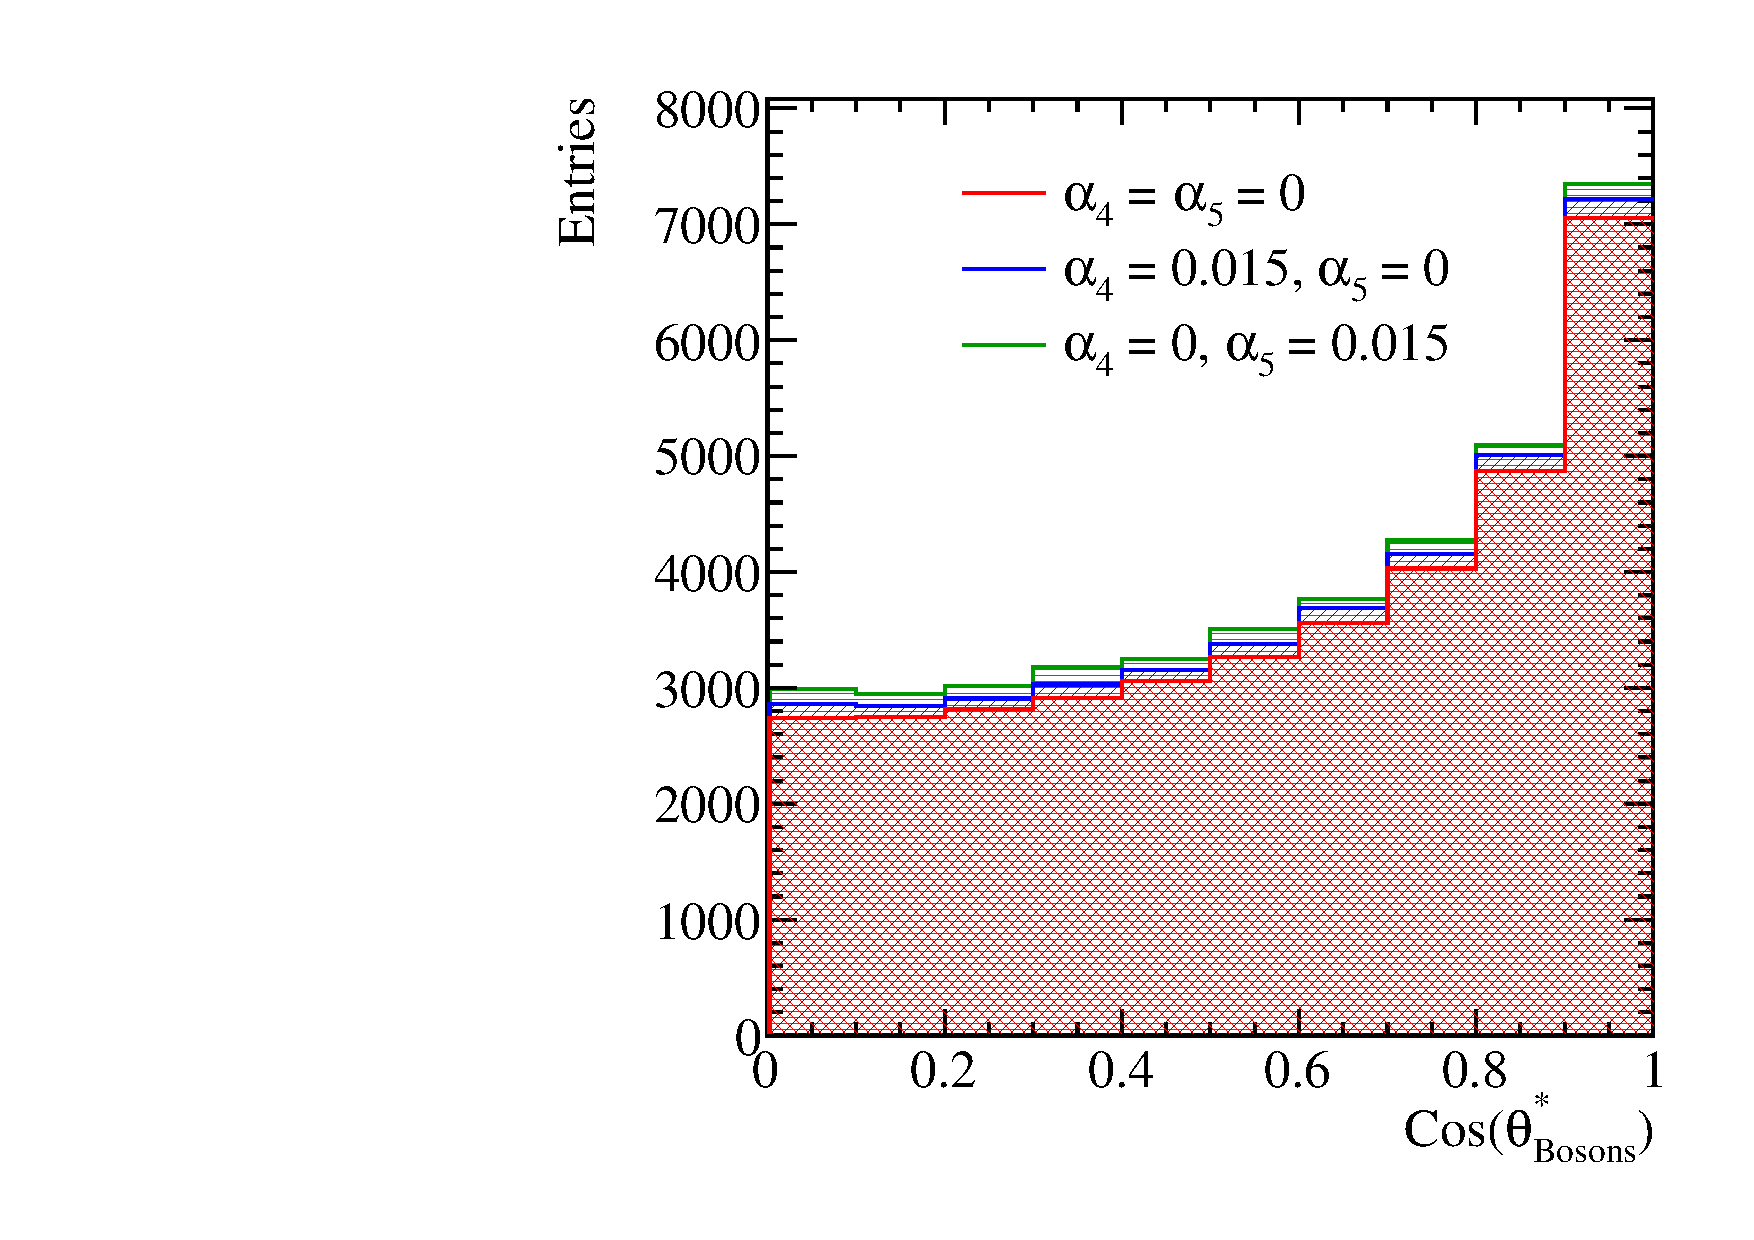
\includegraphics[width=0.5\textwidth]{PhysicsAnalysis/Plots/SensitiveDistributions/CosThetaStarSynBosons_SPFOs_kt_0p90_1400GeV.pdf}}
\caption[The sensitivity of various variables to the anomalous gauge couplings $\alpha_{4}$ and $\alpha_{5}$ at 1.4~TeV.  The jet algorithm used was the longitudinally invariant kt algorithm with an R parameter of 0.9 and Selected PFOs were used.  This distribution is for the \nu{\nu}qqqq signal final state only.  \protect\subref{fig:costhetastarjets1400GeV} shows the distribution of $\text{cos}\theta^{*}_{Jets}$ and \protect\subref{fig:costhetastarbosons1400GeV} shows the distribution of $\text{cos}\theta^{*}_{Bosons}$.]{The sensitivity of various variables to the anomalous gauge couplings $\alpha_{4}$ and $\alpha_{5}$ at 1.4~TeV.  The jet algorithm used was the longitudinally invariant kt algorithm with an R parameter of 0.9 and Selected PFOs were used.  This distribution is for the \nu{\nu}qqqq signal final state only.  \protect\subref{fig:costhetastarjets1400GeV} shows the distribution of $\text{cos}\theta^{*}_{Jets}$ and \protect\subref{fig:costhetastarbosons1400GeV} shows the distribution of $\text{cos}\theta^{*}_{Bosons}$.}
\label{fig:costhetastar}
\end{figure}

%========================================================================================

\subsection{$\chi^{2}$ Surface Definition}
\label{sec:chi2surfacedefinition}
The $\chi^{2}$ surface is defined through the following equation:

\begin{equation}
\chi^{2} = \sum_{i} \frac{(O_{i} - E_{i})^{2}}{E_{i}} \text{,}
\end{equation}

\noindent where $O_{i}$ is the observed, $\alpha_{4} = \alpha_{5} = 0$, and $E_{i}$ the expected, $\alpha_{4} \neq 0$ and $\alpha_{5} \neq 0$, bin content for bin $i$ in the distribution of $M_{VV}$.  $\Sigma_{i}$ is the sum over the bins of the $M_{VV}$ distribution.  The distribution of $M_{VV}$ was binned using 14 bins.  The first bin spanned the invariant mass range between 0 and 200~GeV, this was followed by 11 bins of width 100~GeV ranging from 200 to 1300~GeV and finally the last bin contained all invariant masses above 1300~GeV.  The expanded bin widths were chosen at the tails of the distribution to ensure the bin contents are sufficiently large to give a reliable estimate the likelihood function using the $\chi^{2}$ parameter.  This choice of binning minimises the effect of large bin by bin fluctuations arising from individual events with large event weights.

Confidence limits describing the sensitivity of the CLIC experiment to the anomalous gauge couplings were found by examining this $\chi^{2}$ surface in $\alpha_{4}$ and $\alpha_{5}$ space.  Deviations about the minima of this surface, which by construction occurs at $\alpha_{4} = \alpha_{5} = 0$, yield confidence limits that indicate the probability of observing a particular value of $\alpha_{4}$ and $\alpha_{5}$.  The confidence limits used in subsequent sections, 68\%, 90\% and 99\%, are defined using fixed deviations from the minima of $\chi^{2}$ contours of 2.28, 4.61 and 9.21 respectively.  These numbers arise from the integral of the two dimensional $\chi^{2}$ function.

It proved useful to consider the sensitivities to the individual parameters $\alpha_{4}$ and $\alpha_{5}$ independently.  This was done by projecting out the $\alpha_{4} = 0$ or $\alpha_{5} = 0$ one dimensional $\chi^{2}$ distribution from the two dimensional $\chi^{2}$ distribution as discussed in section \ref{sec:optimaljetalgorithm}.  The sensitivity to individual parameters was then extracted using confidence limits arising from the integral of the one dimensional $\chi^{2}$ function i.e. 68\% confidence limit occurs for $\chi^{2} = 0.989$.  In subsequent chapters these are the sensitivities quoted for individual anomalous gauge couplings. 

%========================================================================================

\subsection{Event Weight Interpolation Scheme}
\label{sec:eventweightsinterpolation}
As described in section \ref{sec:modellingofanomalouscouplings}, event weights are used to determine the sensitivity of CLIC to the anomalous gauge couplings.  These event weights are extracted on an event by event basis for the signal final state $\nu\nu\text{qqqq}$ from the generator Whizard.  To achieve a smooth $\chi^{2}$ distribution a fine sampling of the $M_{VV}$ distribution in the $\alpha_{4}$ and $\alpha_{5}$ space is needed.  However, as extracting the event weights is highly CPU intensive, it is unfeasible to produce a finely sampled grid of event weights on an event by event basis by calling the generator.  To resolve this issue, an interpolation scheme was applied to determine the event weights within a sampled region of the $\alpha_{4}$ and $\alpha_{5}$ space.  This allows for an infinite sampling of the $M_{VV}$ distribution in the space of $\alpha_{4}$ and $\alpha_{5}$ within the sampled region, without having to call the generator an infinite number of times.

A bicubic interpolation scheme, cubic interpolation along two dimensions, was applied to the event weights that were extracted from the generator.  This procedure is best illustrated by figure \ref{fig:eventweights1400interpolated}, which shows the interpolated event weight surface superimposed with the raw event weights from the generator for several $\nu\nu\text{qqqq}$ events at 1.4~TeV.  This interpolation scheme produces a smooth and continuous surface that is sufficiently accurate for the fitting procedure applied in this analysis.  At 1.4~TeV event weights were produced from the generator, Whizard, by stepping along $\alpha_{4}$ and $\alpha_{5}$ in steps of 0.01 ranging from -0.07 to 0.07, as shown in figure \ref{fig:eventweights1400raw}.  These range proved to be sufficient for the contours of interest for the CLIC sensitivity analysis at these energies.

\begin{figure}[h!]
\centering
\subfloat[]{\label{fig:weight1}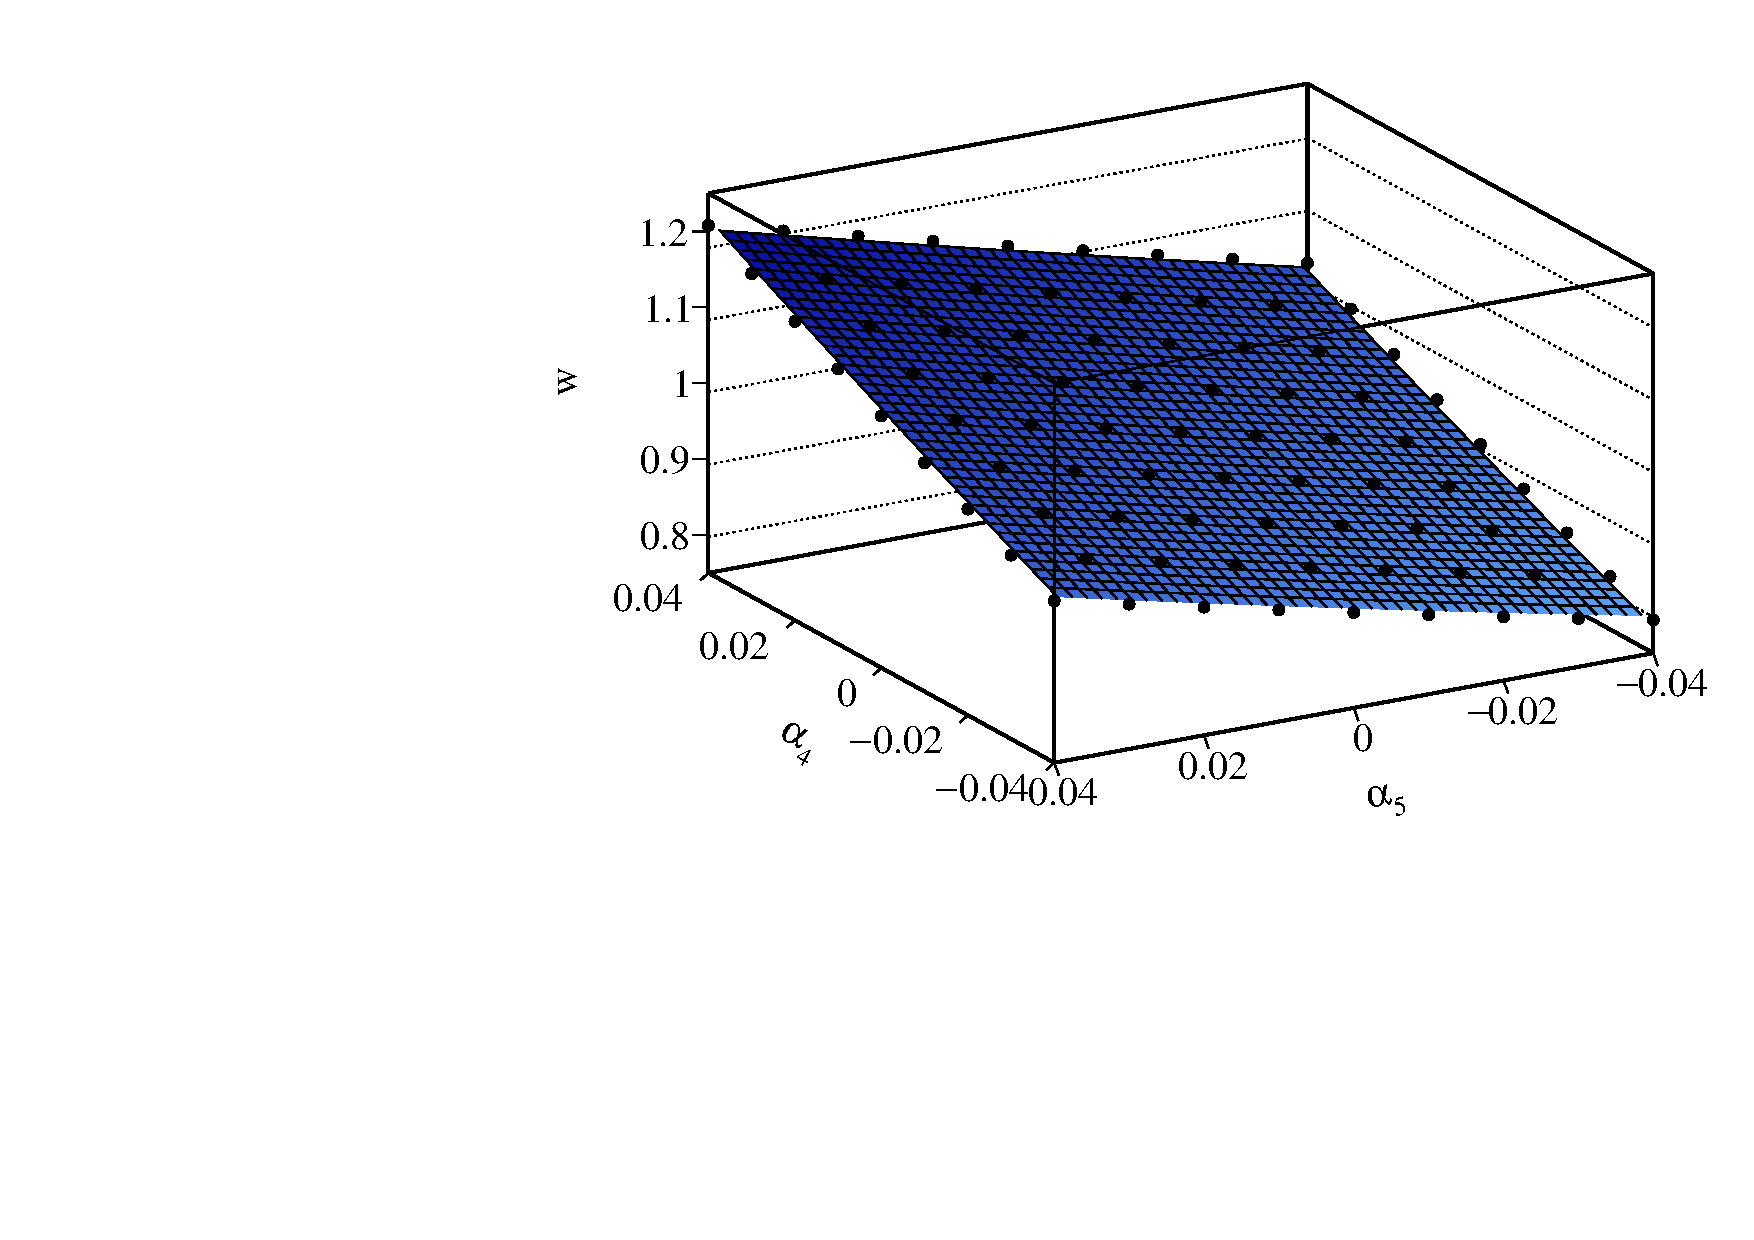
\includegraphics[width=0.5\textwidth]{PhysicsAnalysis/Plots/EventWeights/1400GeV/EventWeightsForEvent100001009_1400GeV_SPFOs_kt_0p70_10Bins_Start_0_End_10_1400GeV_Interpolated.pdf}}
\subfloat[]{\label{fig:weight2}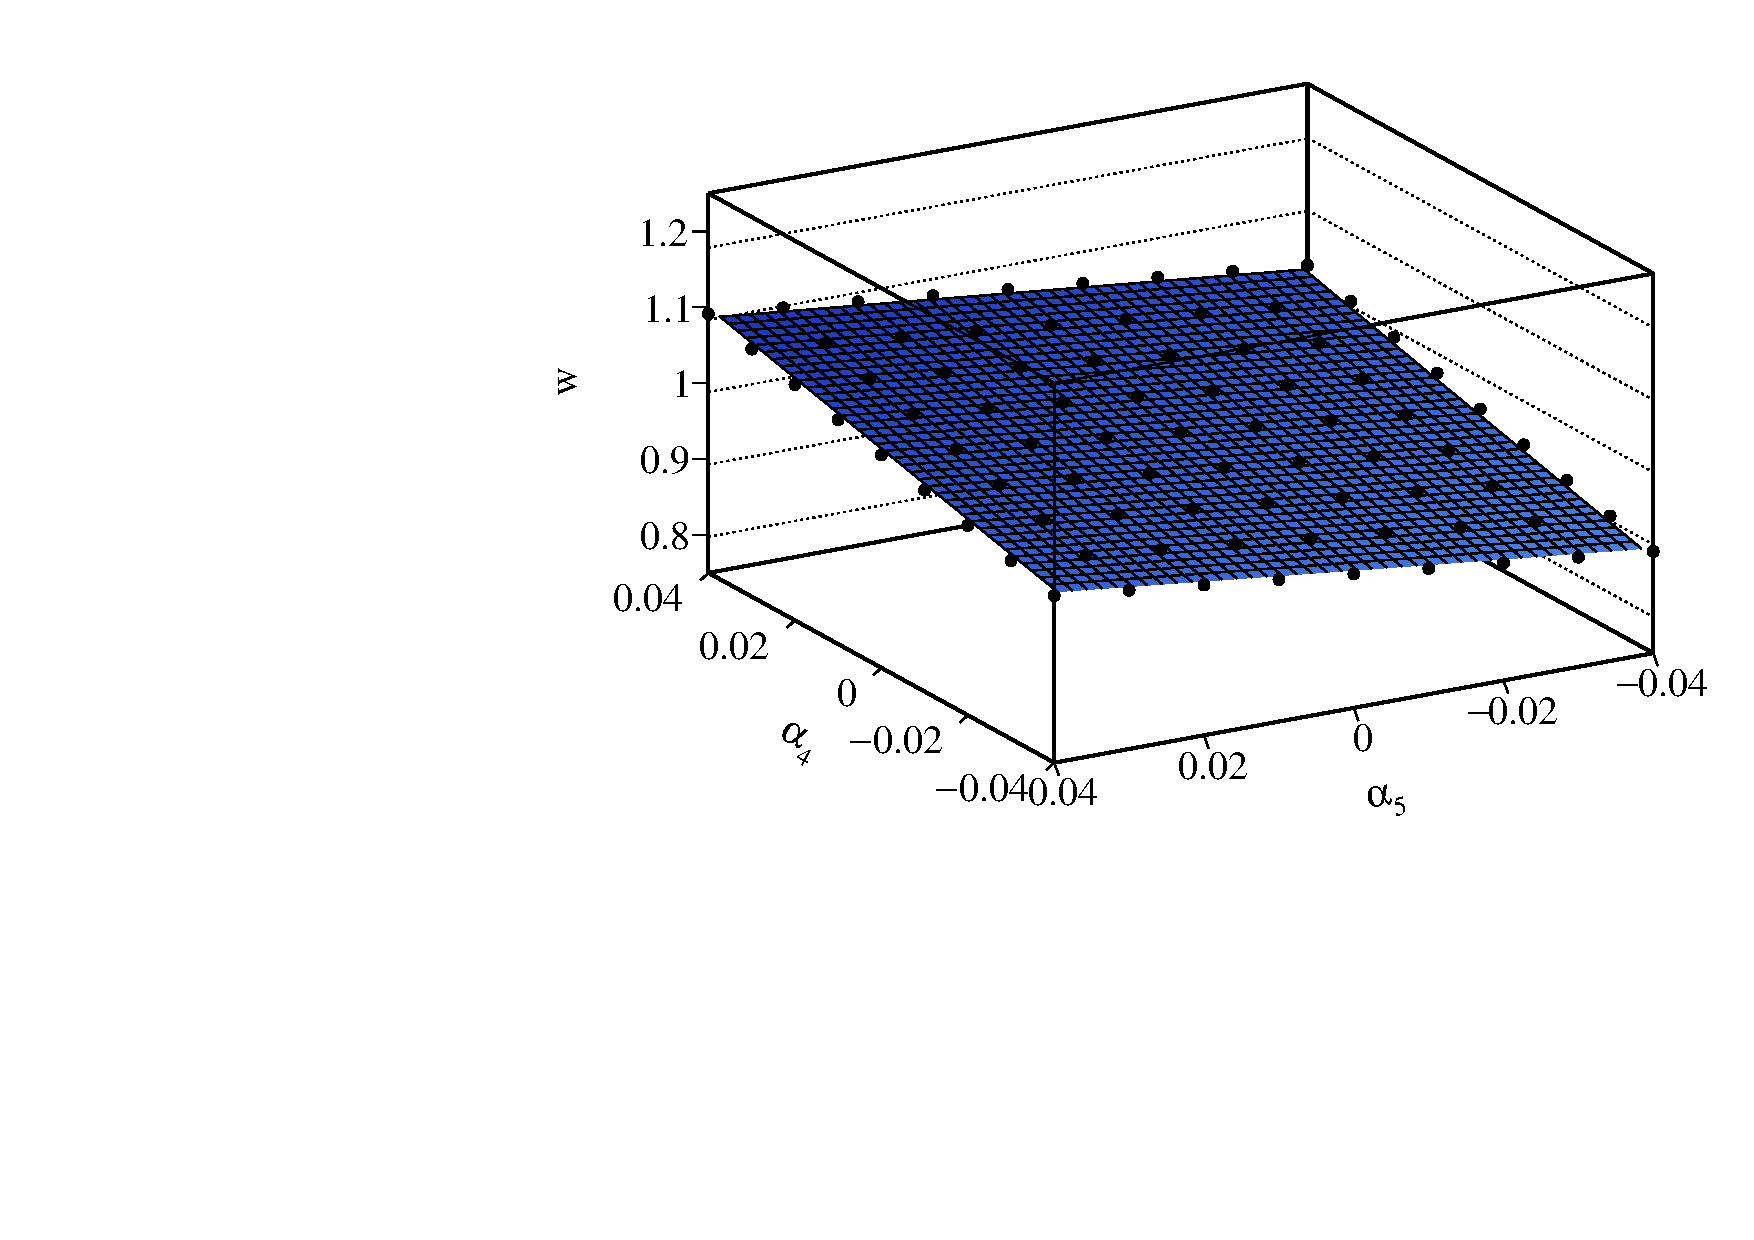
\includegraphics[width=0.5\textwidth]{PhysicsAnalysis/Plots/EventWeights/1400GeV/EventWeightsForEvent100001014_1400GeV_SPFOs_kt_0p70_10Bins_Start_0_End_10_1400GeV_Interpolated.pdf}} \hfill
\subfloat[]{\label{fig:weight3}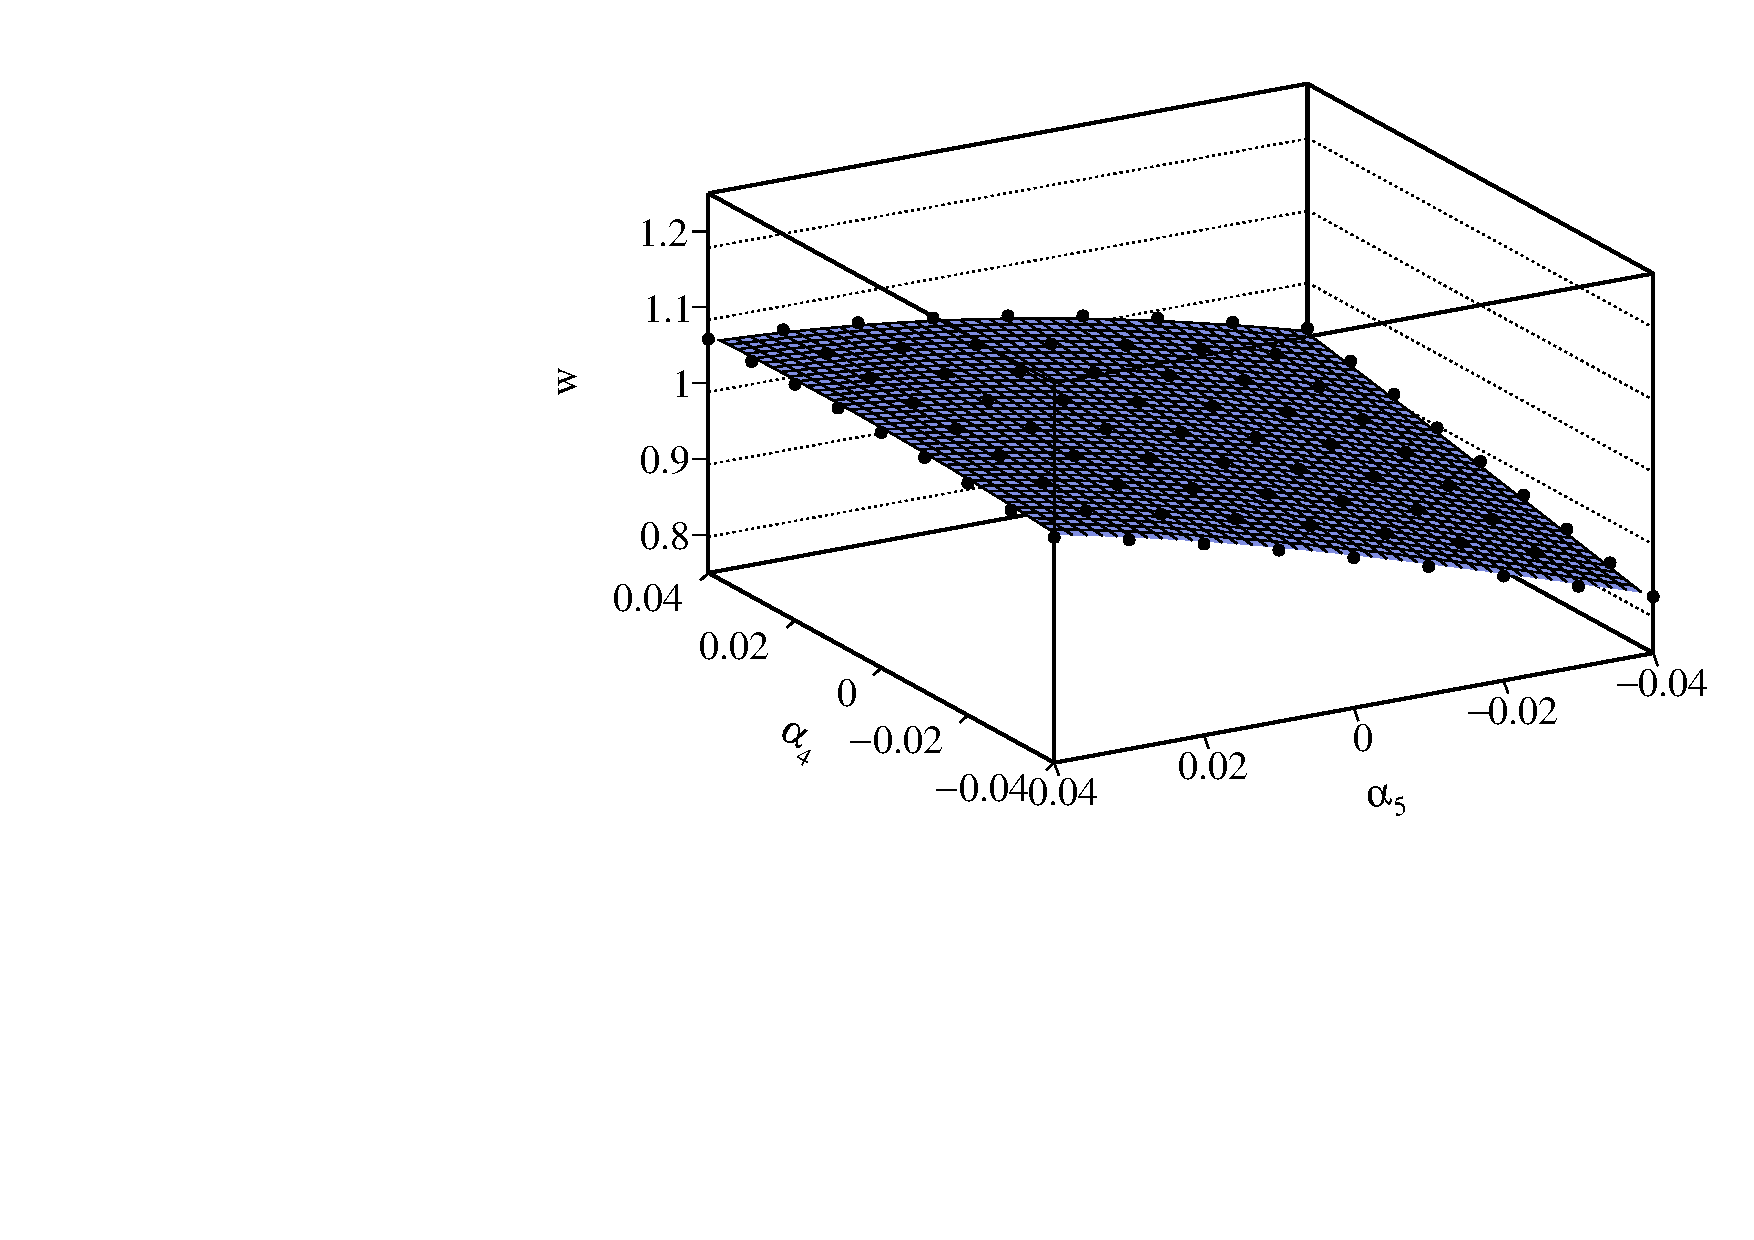
\includegraphics[width=0.5\textwidth]{PhysicsAnalysis/Plots/EventWeights/1400GeV/EventWeightsForEvent100001044_1400GeV_SPFOs_kt_0p70_10Bins_Start_0_End_10_1400GeV_Interpolated.pdf}}
\subfloat[]{\label{fig:weight4}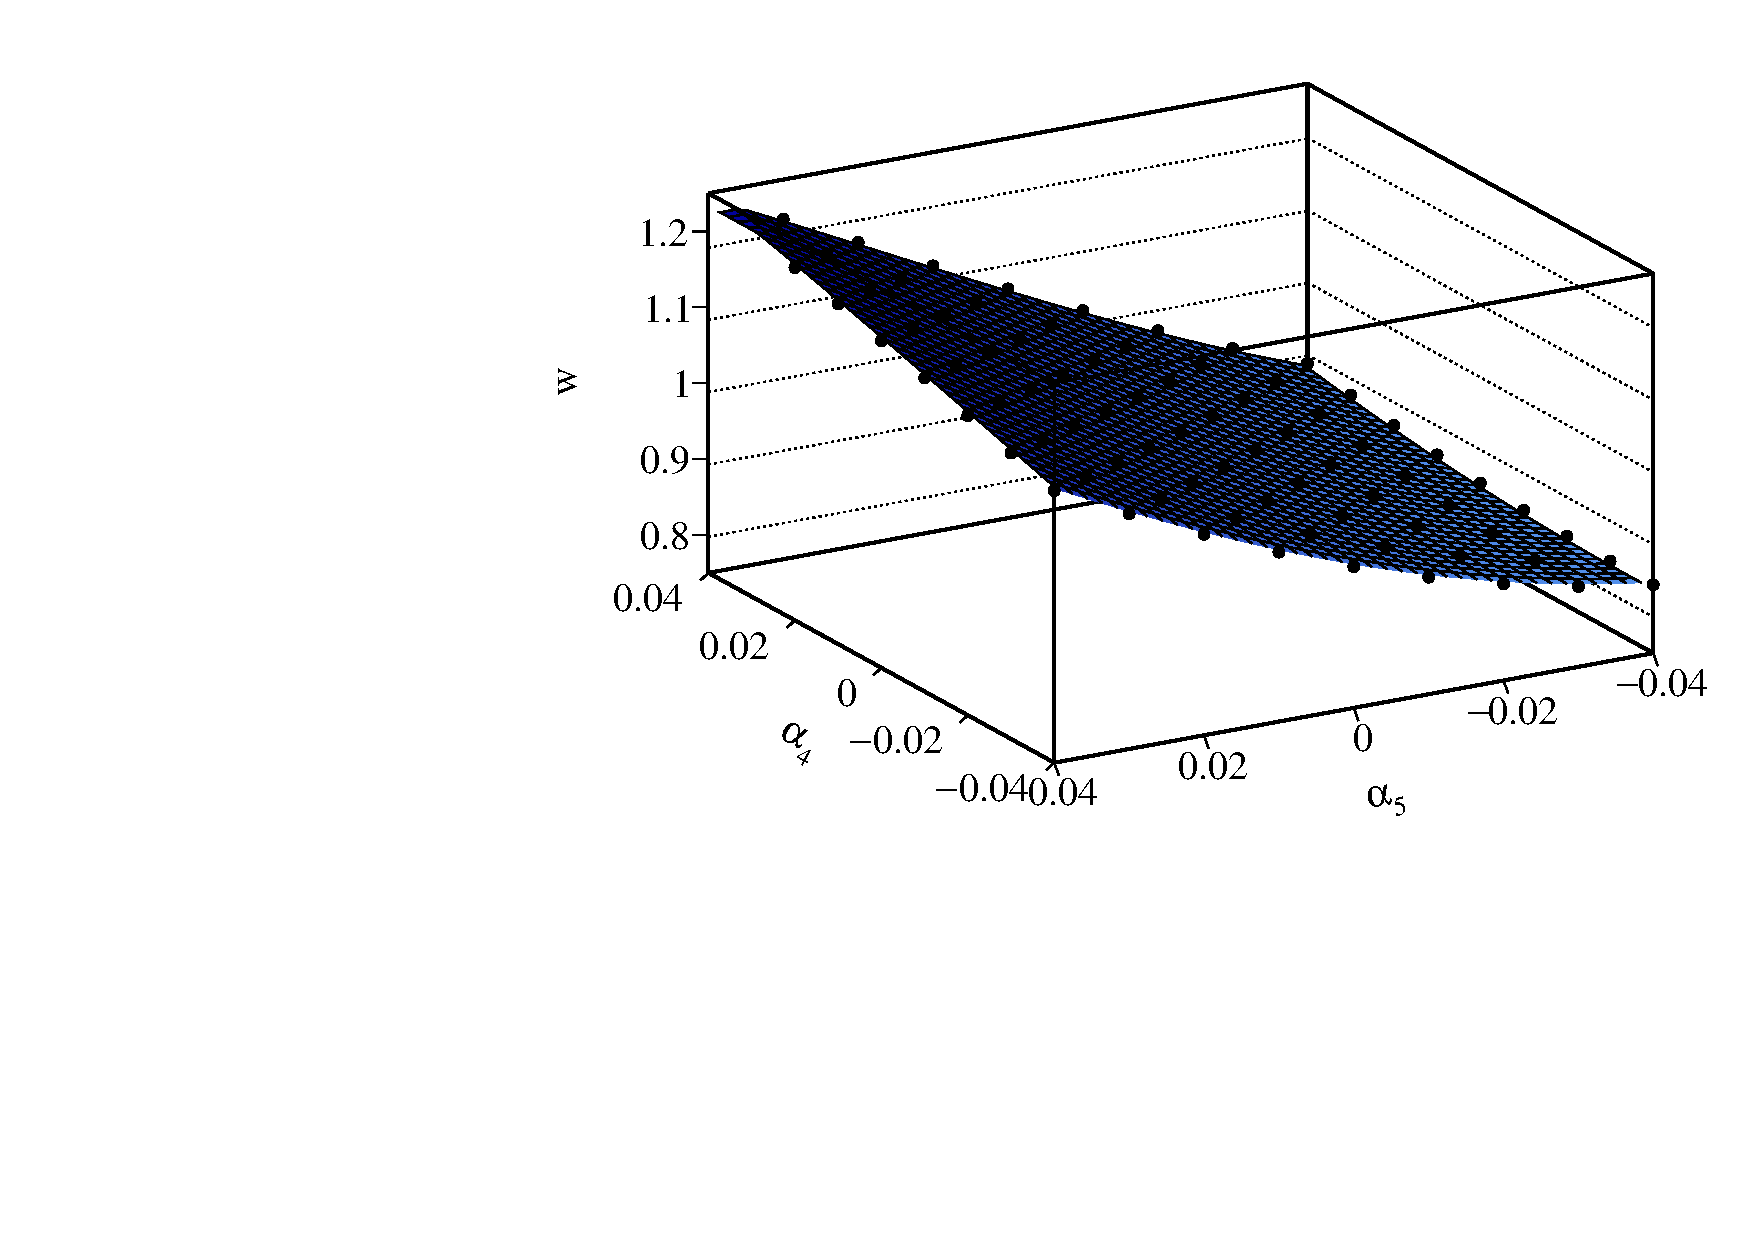
\includegraphics[width=0.5\textwidth]{PhysicsAnalysis/Plots/EventWeights/1400GeV/EventWeightsForEvent100001051_1400GeV_SPFOs_kt_0p70_10Bins_Start_0_End_10_1400GeV_Interpolated.pdf}}
\caption[A selection of plots showing how the event weight changes when varying the anomalous couplings $\alpha_{4}$ and $\alpha_{5}$ for 1.4~TeV \nu{\nu}qqqq final state events.  The hollow circles show the event weight produced from the generator, while the surface shown is found using bicubic interpolation between those points.]{A selection of plots showing how the event weight changes when varying the anomalous couplings $\alpha_{4}$ and $\alpha_{5}$ for 1.4~TeV \nu{\nu}qqqq final state events.  The hollow circles show the event weight produced from the generator, while the surface shown is found using bicubic interpolation between those points.}
\label{fig:eventweights1400interpolated}
\end{figure}

%========================================================================================
%========================================================================================

\section{Results}
The sensitivity of the CLIC experiment to the anomalous gauge couplings $\alpha_{4}$ and $\alpha_{5}$ at 1.4~TeV is shown in figure \ref{fig:finalresult1400GeV}.  This result shows the sensitivity after the application of preselection and MVA purposed to remove the included background channels.  These contours yield the one $\sigma$ confidence limit on the measurement of $\alpha_{4}$ to the range -0.0082, 0.0116 and similarly for the measurement of $\alpha_{5}$ to the range -0.0055, 0.0078.

\begin{figure}[h!]
\centering
\subfloat[]{\label{fig:finalresult1400GeV}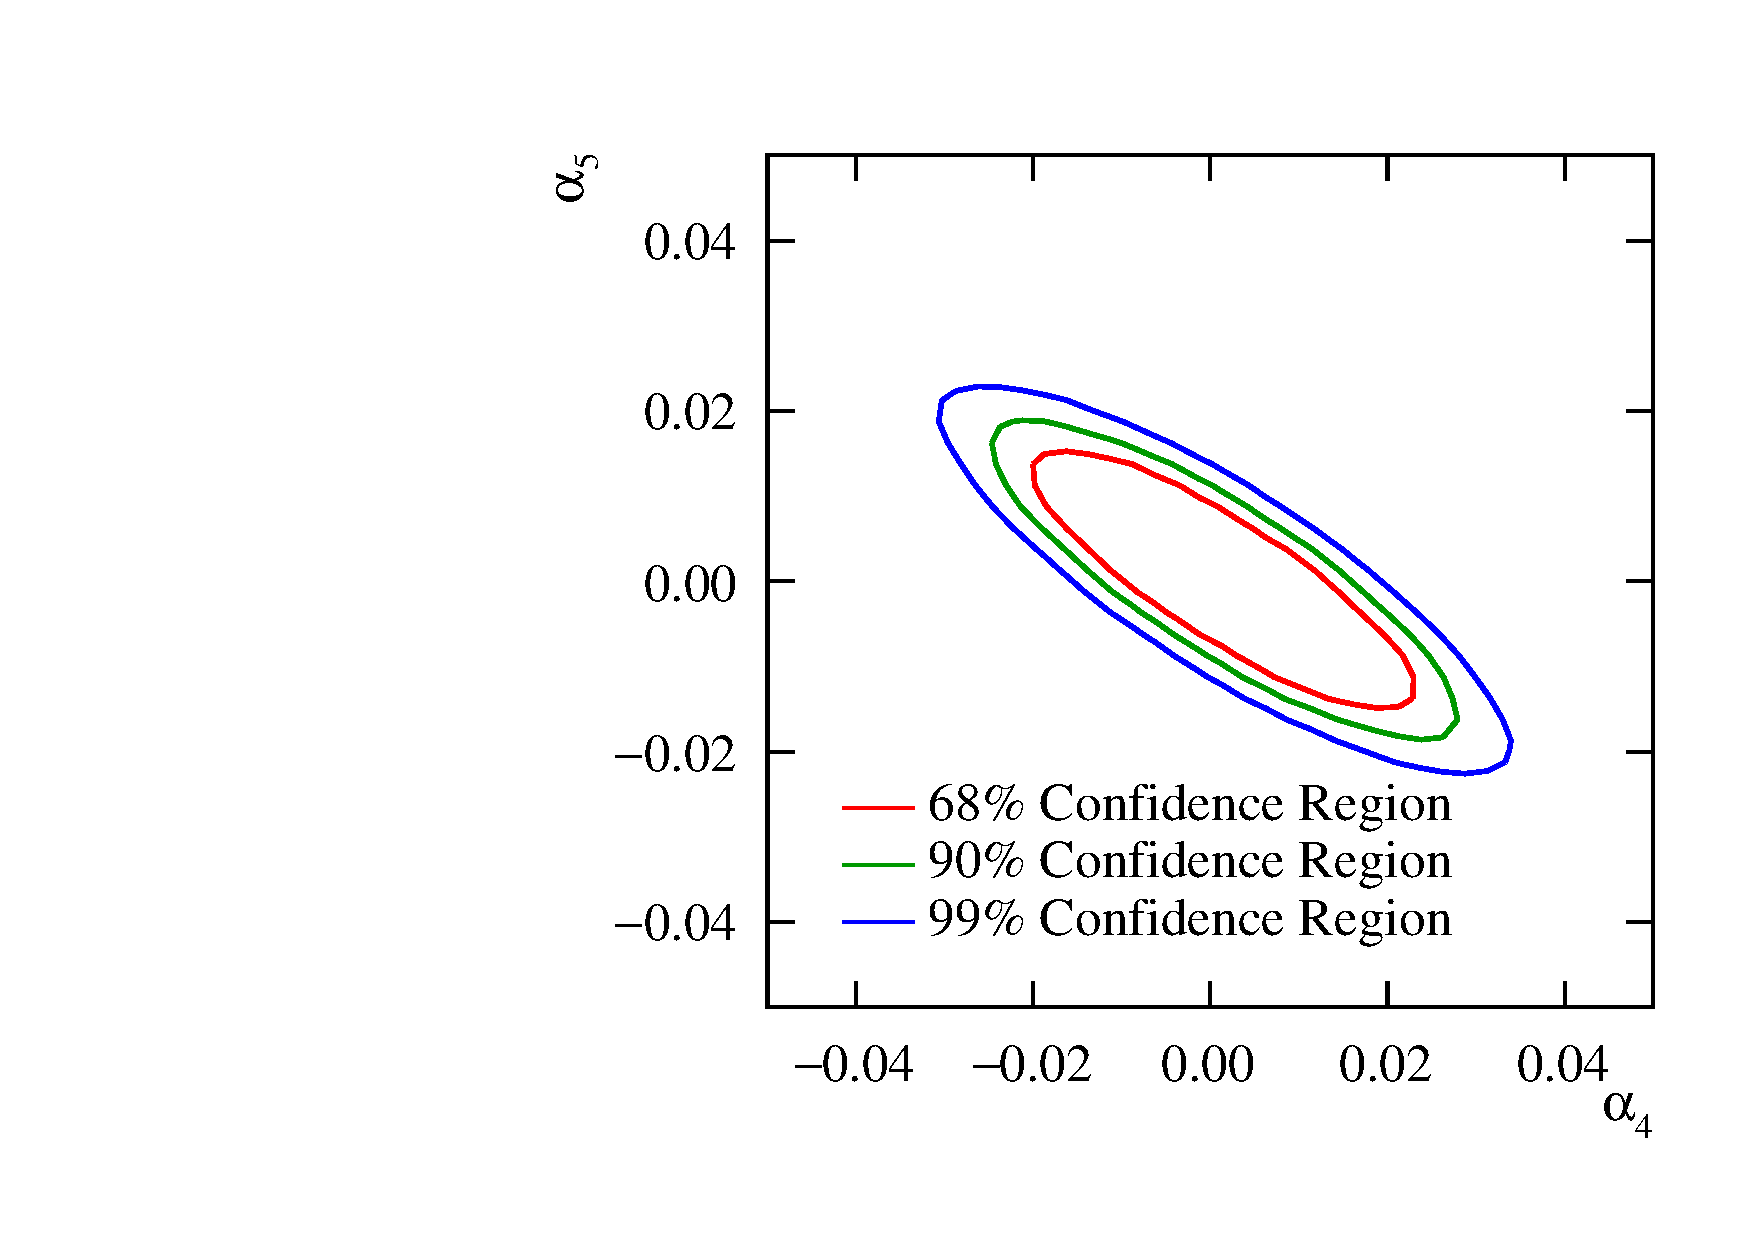
\includegraphics[width=0.5\textwidth]{PhysicsAnalysis/Plots/FinalResult/1400GeV/Final.pdf}}\hfill
\subfloat[]{\label{fig:a4finalresult1400GeV}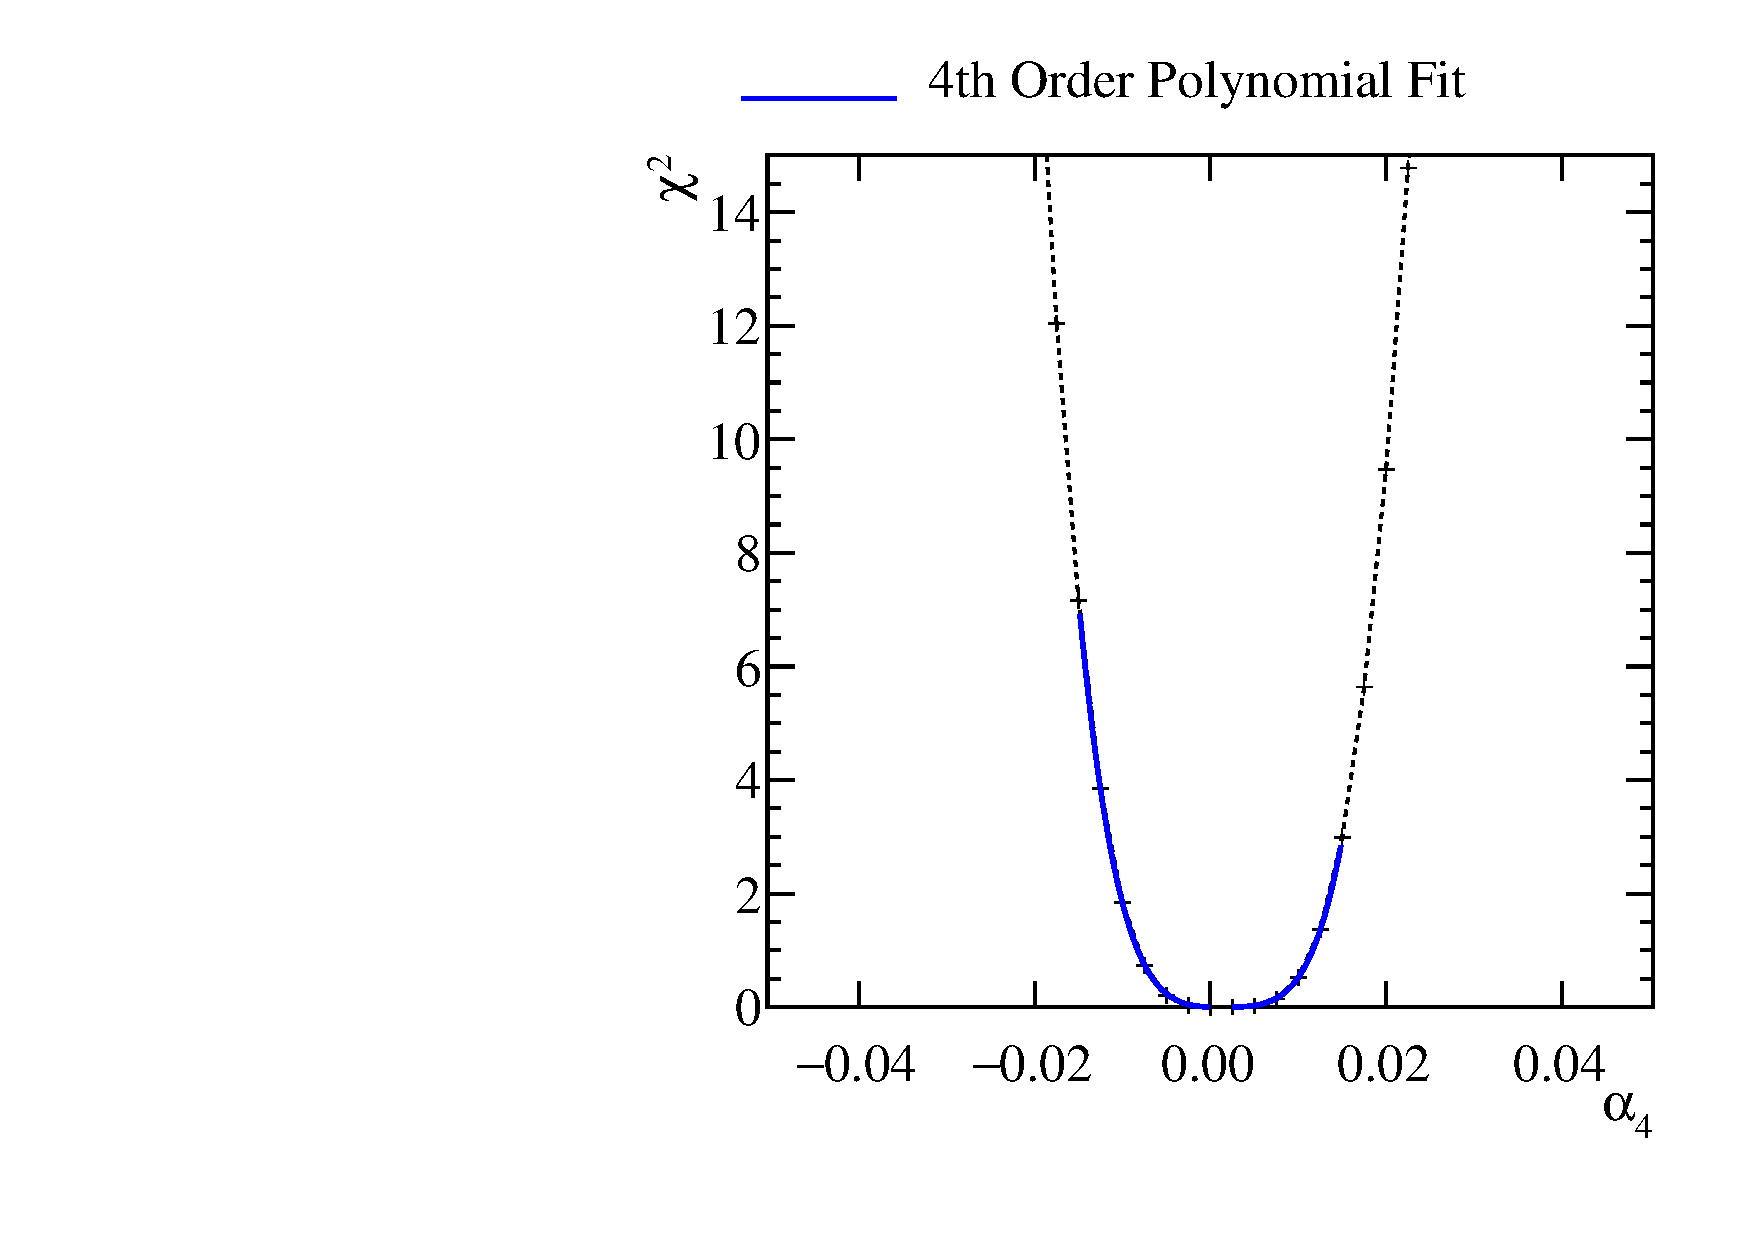
\includegraphics[width=0.5\textwidth]{PhysicsAnalysis/Plots/FinalResult/1400GeV/Final_alpha4.pdf}}
\subfloat[]{\label{fig:a5finalresult1400GeV}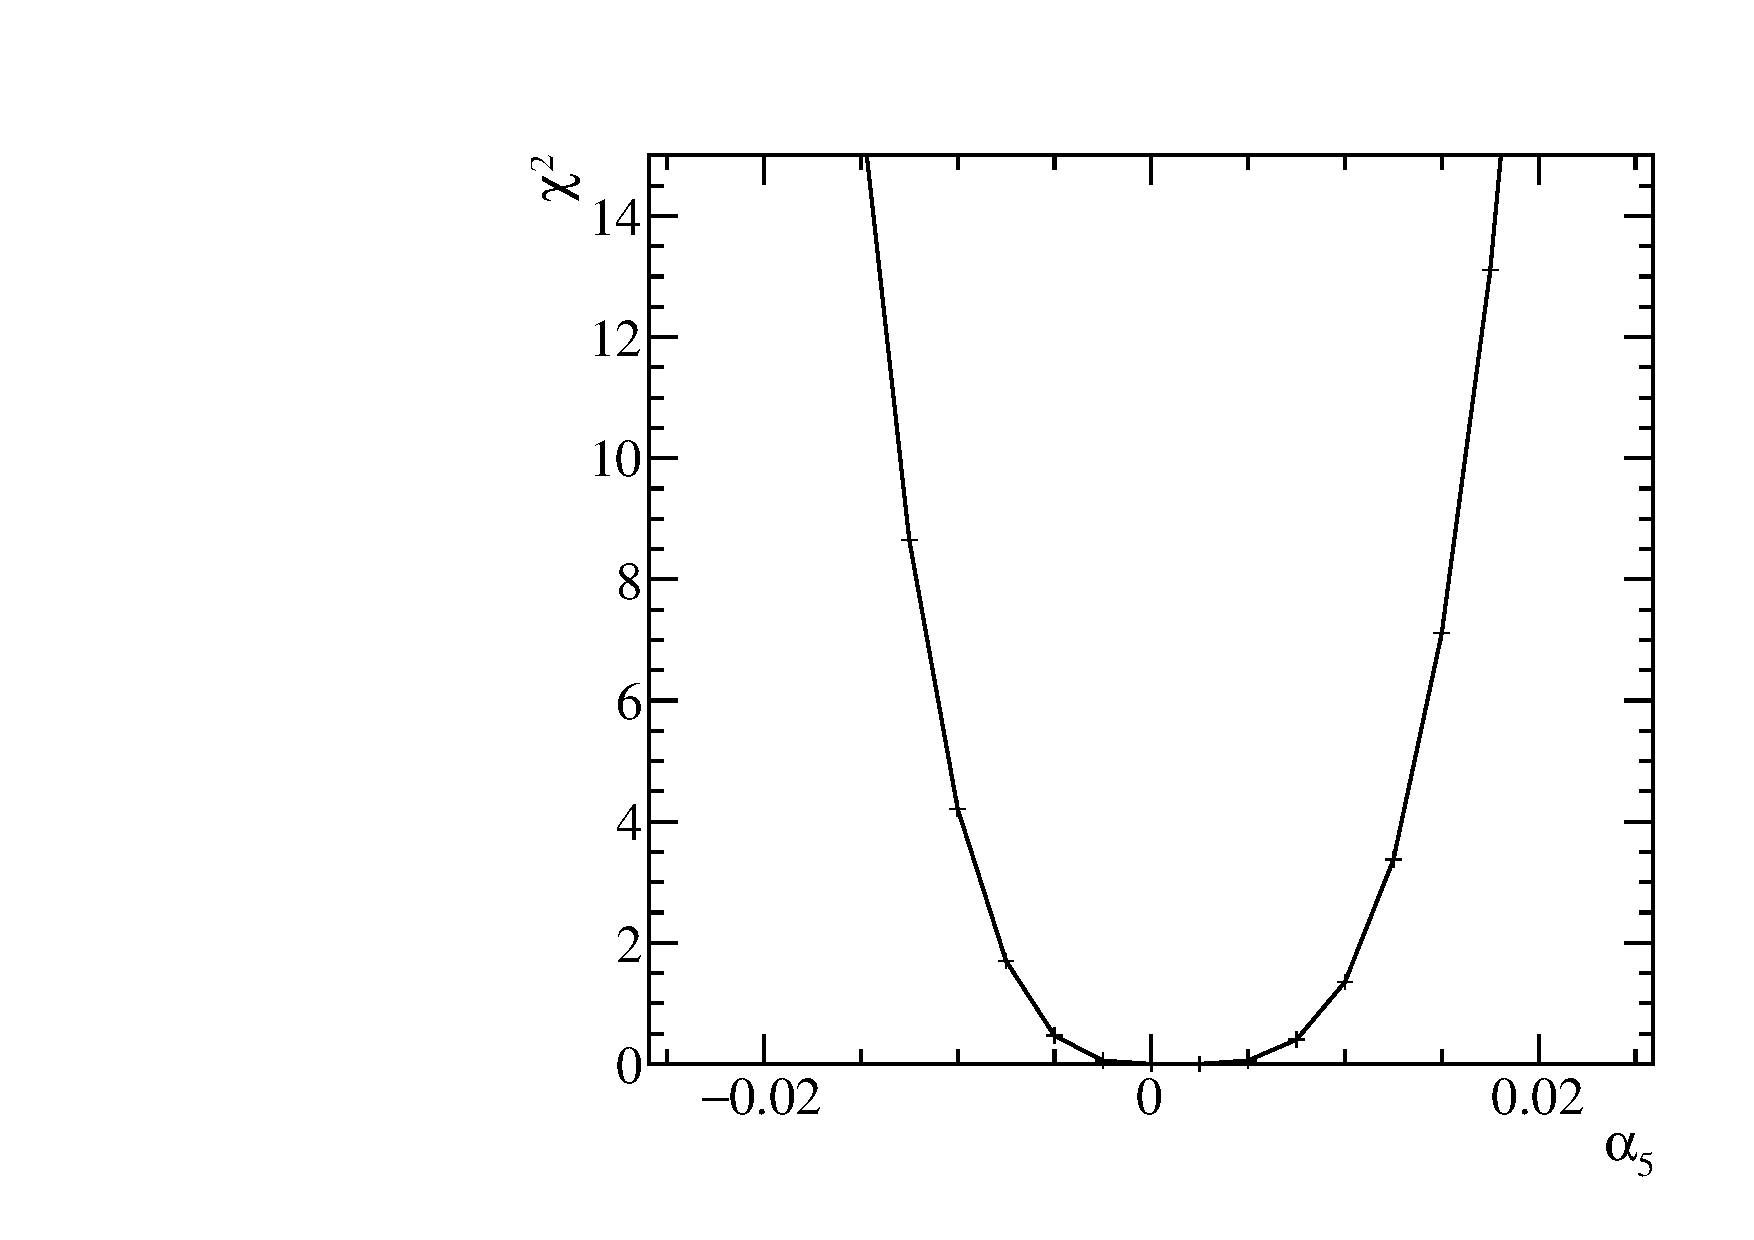
\includegraphics[width=0.5\textwidth]{PhysicsAnalysis/Plots/FinalResult/1400GeV/Final_alpha5.pdf}}
\caption[$\chi^{2}$ sensitivity distributions from a fit to $M_{VV}$ at 1.4~TeV.  Results include the effect of backgrounds after the application of a series of preselection cuts and MVA.  \protect\subref{fig:finalresult1400GeV} $\chi^{2}$ sensitivity contours in $\alpha_{4}$ and $\alpha_{5}$ space.  \protect\subref{fig:a4finalresult1400GeV} $\chi^{2}$ as a function of $\alpha_{4}$ assuming $\alpha_{5} = 0$.  \protect\subref{fig:a5finalresult1400GeV} $\chi^{2}$ as a function of $\alpha_{5}$ assuming $\alpha_{4} = 0$.]{$\chi^{2}$ sensitivity distributions from a fit to $M_{VV}$ at 1.4~TeV.  Results include the effect of backgrounds after the application of a series of preselection cuts and MVA.  \protect\subref{fig:finalresult1400GeV} $\chi^{2}$ sensitivity contours in $\alpha_{4}$ and $\alpha_{5}$ space.  \protect\subref{fig:a4finalresult1400GeV} $\chi^{2}$ as a function of $\alpha_{4}$ assuming $\alpha_{5} = 0$.  \protect\subref{fig:a5finalresult1400GeV} $\chi^{2}$ as a function of $\alpha_{5}$ assuming $\alpha_{4} = 0$.}
\label{fig:allfinalresult1400GeV}
\end{figure}

%========================================================================================

\subsection{Systematic Uncertainties}
A source of systematic error in this experiment is the uncertainty on the cross sections for the signal and background final states.  Based on the selection efficiencies given in table \ref{table:selectionsummary1400GeV}, the $\chi^{2}$ fit procedure is applied on a distribution that primarily consists of the background final states $\text{qqqq}\nu$ arising from the interaction of $\text{e}^{+}$ and $\text{e}^{-}$ with beamstrahlung photons.  Therefore, uncertainties in the cross section for these backgrounds should be considered.  A detailed study of the accuracy of the relevant cross section calculations has yet to be performed for CLIC and so a wide spectrum in the uncertainty of these cross sections is considered here.   

This systematic is included in the $\chi^{2}$ through the use of a nuisance parameter, whereby the cross section for the $\gamma_{\text{BS}}\text{e}^{\pm} \rightarrow \text{qqqq}\nu$ backgrounds are allowed to fluctuate.  The magnitude of the fluctuation of the cross section, $r$, is moderated by an additional penalty term in the $\chi^{2}$ as follows:

\begin{equation}
\chi^{2}(r) = \sum_{i} \frac{(O_{i} - E_{i}(r))^{2}}{E_{i}(r)} + \frac{(r-1)^{2}}{\sigma_{r}^{2}} \text{,}
\end{equation}

\noindent where $O_{i}$ is the observed, $\alpha_{4} = \alpha_{5} = 0$, bin content for bin $i$ in the distribution of $M_{VV}$ with no background fluctuations.  $E_{i}(r)$ is the expected, $\alpha_{4} \neq 0$ and $\alpha_{5} \neq 0$, bin content for bin $i$ in the distribution of $M_{VV}$ with the $\gamma_{\text{BS}}\text{e}^{\pm} \rightarrow \text{qqqq}\nu$ background cross sections fluctuated by the factor $r$.  $\sum_{i}$ is the sum over the bins of the $M_{VV}$ distribution.  $\sigma_{r}$ is the width of the distribution of $r$, which indicates the uncertainty on the measurement of the background cross sections.  The $\chi^{2}$ surface is constructed in the space of $\alpha_{4}$ and $\alpha_{5}$ by minimising $\chi^{2}(r)$ at each point.  The 68\% confidence contour is shown with the inclusion of this nuisance parameter for various values of $\sigma_{r}$ in figure \ref{fig:nuisance1400GeV}.   

\begin{figure}[h!]
\centering
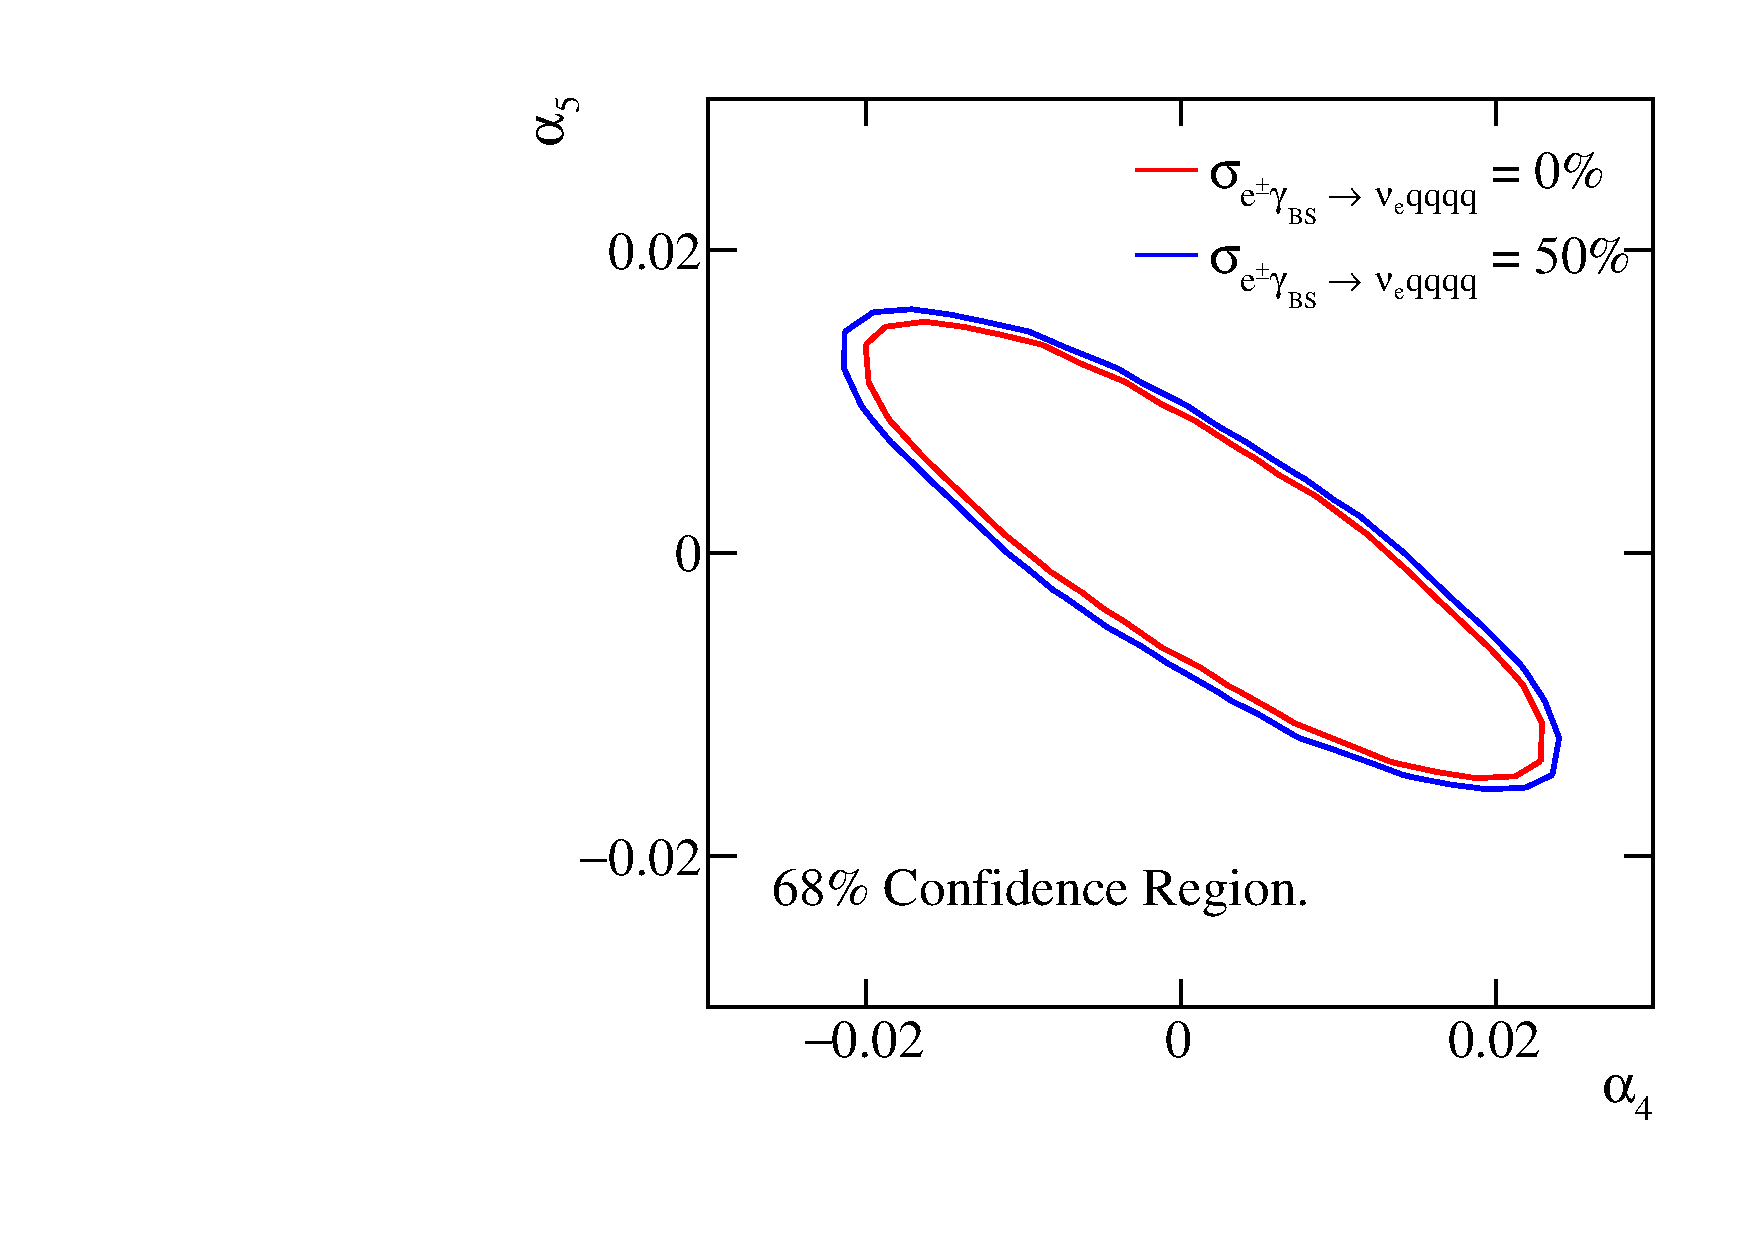
\includegraphics[width=0.5\textwidth]{PhysicsAnalysis/Plots/NuisanceFit/1400GeV/Nuisance.pdf}
\caption[68\% sensitivity contour including systematic errors, of varying magnitudes, in dominant background cross sections.]{68\% sensitivity contour including systematic errors, of varying magnitudes, in dominant background cross sections.}
\label{fig:nuisance1400GeV}
\end{figure}

Minimal changes in sensitivity are observed when allowing the backgrounds to fluctuate even up to the 50\% level.  This can be understood by considering the shape of the $M_{VV}$ distribution for the signal, with and without the effect of anomalous couplings, and the $\gamma_{\text{BS}}\text{e}^{\pm} \rightarrow \text{qqqq}\nu$ backgrounds, which is shown in figure \ref{fig:nuisanceexplanation1400GeV}.  These distribution shows that anomalous couplings primarily affect events with large invariant masses, while these backgrounds peak at low invariant masses.  Therefore, by fluctuating the cross-section for the background processes it is not possible to gain a significantly better match between the observed and expected bin contents in the $M_{VV}$ distribution.  This is encouraging as despite these backgrounds dominating the fit being used to determine the sensitivity of CLIC to the anomalous gauge couplings, precise knowledge of their cross-section is not essential.

\begin{figure}[h!]
\centering
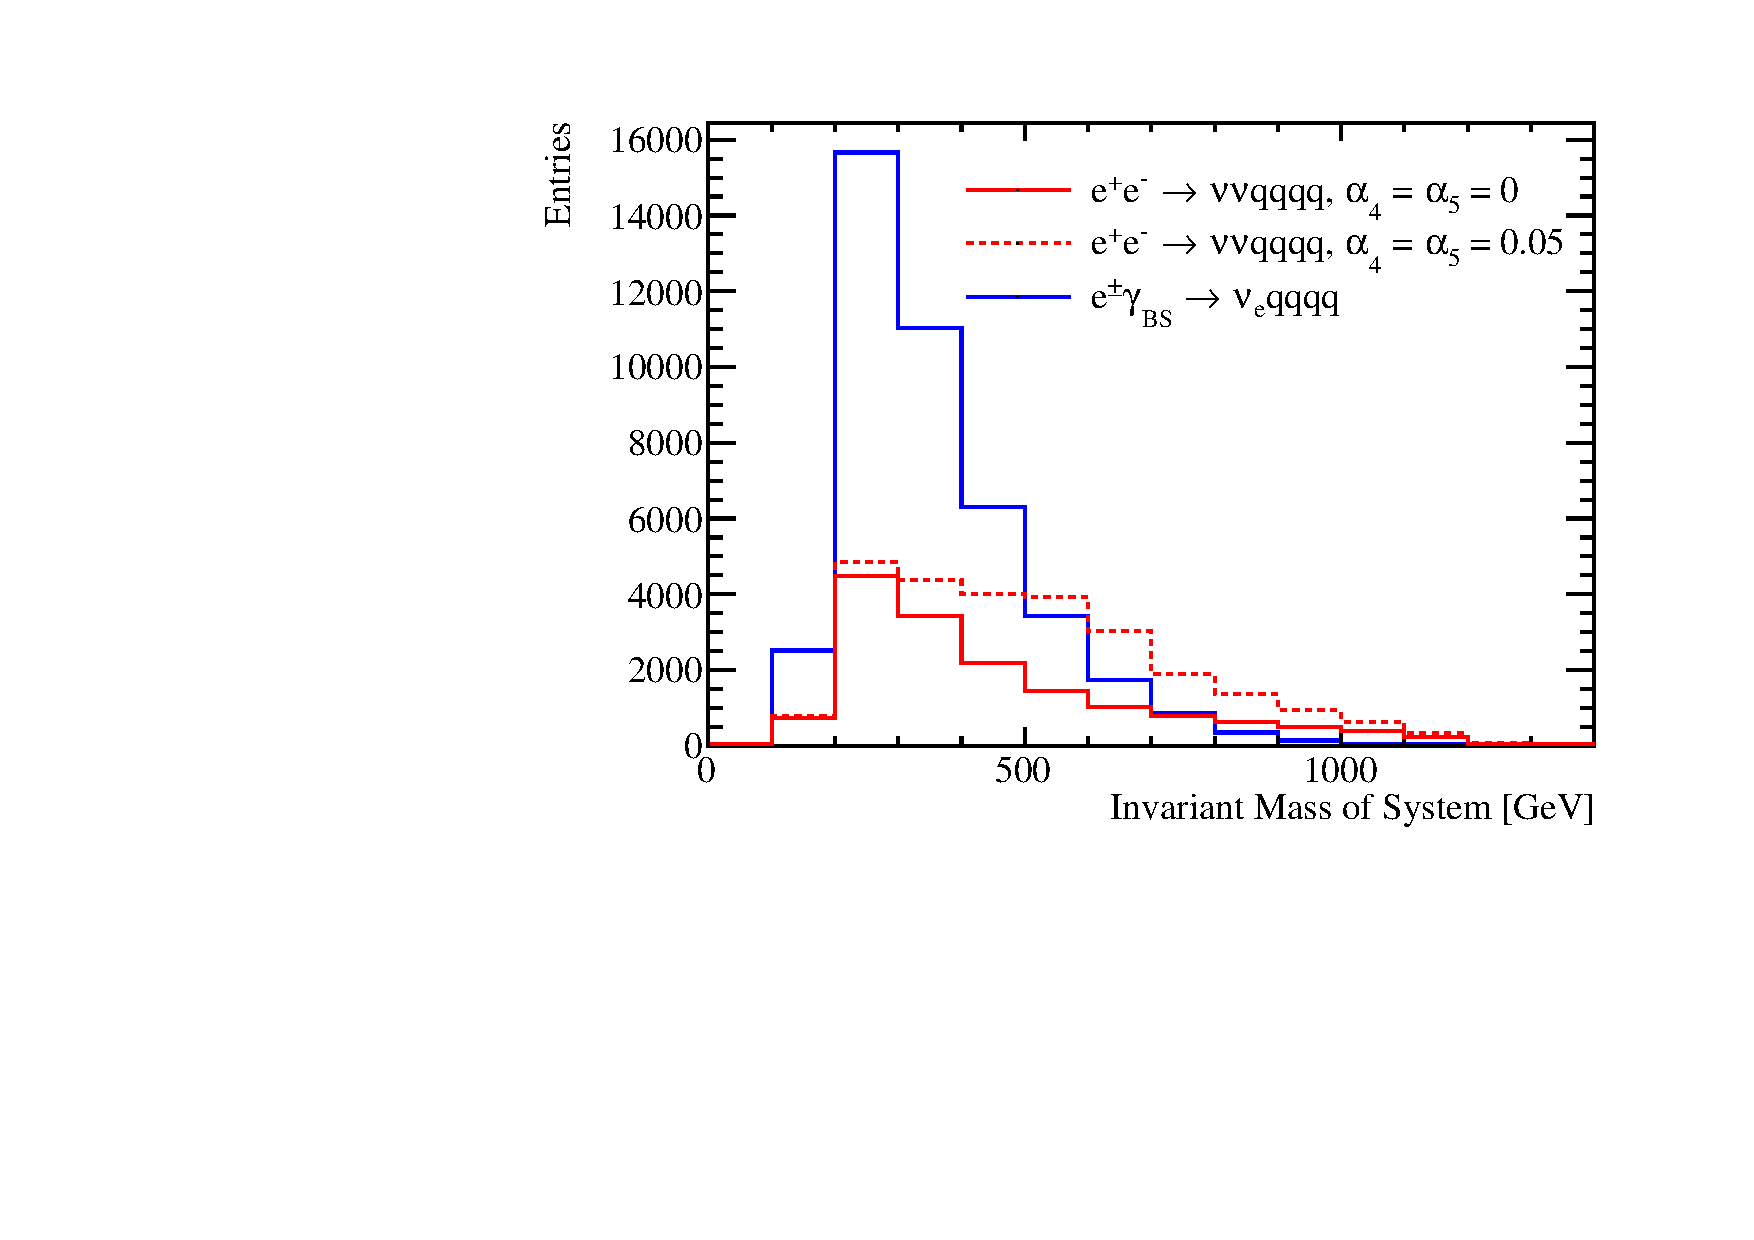
\includegraphics[width=0.75\textwidth]{PhysicsAnalysis/Plots/NuisanceFit/1400GeV/NuisanceExplanation.pdf}
\caption[Distributions of $M_{VV}$ for the $\nu\nu\text{qqqq}$, with and without the effect from anomalous couplings, and the combined dominant background processes $\gamma_{\text{BS}}\text{e}^{\pm} \rightarrow \text{qqqq}\nu$.]{Distributions of $M_{VV}$ for the $\nu\nu\text{qqqq}$, with and without the effect from anomalous couplings, and the combined dominant background processes $\gamma_{\text{BS}}\text{e}^{\pm} \rightarrow \text{qqqq}\nu$.}
\label{fig:nuisanceexplanation1400GeV}
\end{figure}

%========================================================================================
%========================================================================================

\section{Sensitivity at 3~TeV}
The anomalous gauge coupling sensitivity study described in this chapter was reproduced for CLIC operating at 3~TeV.  The procedure for the 3~TeV analysis largely mirrors that of the 1.4~TeV analysis, therefore, in this section only the differences between the analyses are highlighted.  

The signal and background final states for the 3~TeV analysis were identical to those used for the 1.4~TeV analysis as described in section \ref{sec:eventgenerationandbackgrounds}.  The cross sections at 3~TeV for those signal and background final states can be found in table \ref{table:crosssection3000GeV}.  

\begin{table}[h!]
\centering
\begin{tabular}{ l r r }
\hline
Final State & Cross Section 3~TeV [fb]  \\ 
\hline
$\text{e}^{+}\text{e}^{-} \rightarrow \nu{\nu}\text{qqqq}$ & 71.5 \\
$\text{e}^{+}\text{e}^{-} \rightarrow \text{l}\nu\text{qqqq}$ & 106.6 \\
$\text{e}^{+}\text{e}^{-} \rightarrow \text{llqqqq}$ & 169.3 \\
$\text{e}^{+}\text{e}^{-} \rightarrow \text{qqqq}$ & 546.5 \\
$\text{e}^{+}\text{e}^{-} \rightarrow \nu{\nu}\text{qq}$ & 1317.5 \\
$\text{e}^{+}\text{e}^{-} \rightarrow \text{l}\nu\text{qq}$ & 5560.9 \\
$\text{e}^{+}\text{e}^{-} \rightarrow \text{llqq}$ & 3319.6 \\
$\text{e}^{+}\text{e}^{-} \rightarrow \text{qq}$ & 2948.9 \\
$\gamma_{\text{EPA}}\text{e}^{-} \rightarrow \text{qqqq}\text{e}^{-}$ & 287.8 \\
$\gamma_{\text{BS}}\text{e}^{-} \rightarrow \text{qqqq}\text{e}^{-}$ & 1268.6 \\
$\text{e}^{+}\gamma_{\text{EPA}} \rightarrow \text{qqqq}\text{e}^{+}$ & 287.8 \\
$\text{e}^{+}\gamma_{\text{BS}} \rightarrow \text{qqqq}\text{e}^{+}$ & 1267.3 \\
$\gamma_{\text{EPA}}\text{e}^{-} \rightarrow \text{qqqq}\nu$ & 54.2 \\
$\gamma_{\text{BS}}\text{e}^{-} \rightarrow \text{qqqq}\nu$ & 262.5 \\
$\text{e}^{+}\gamma_{\text{EPA}} \rightarrow \text{qqqq}\nu$ & 54.2 \\
$\text{e}^{+}\gamma_{\text{BS}} \rightarrow \text{qqqq}\nu$ & 262.3 \\
$\gamma_{\text{EPA}}\gamma_{\text{EPA}} \rightarrow \text{qqqq}$ & 402.7 \\
$\gamma_{\text{EPA}}\gamma_{\text{BS}} \rightarrow \text{qqqq}$ & 2423.1 \\
$\gamma_{\text{BS}}\gamma_{\text{EPA}} \rightarrow \text{qqqq}$ & 2420.6 \\
$\gamma_{\text{BS}}\gamma_{\text{BS}} \rightarrow \text{qqqq}$ & 13050.3 \\
\hline
\end{tabular}
\caption[Cross sections of signal and background processes at 3~TeV]{Cross sections of signal and background processes at 3~TeV.  In the above table q represents u, $\bar{\text{u}}$, d, $\bar{\text{d}}$, s, $\bar{\text{s}}$, c, $\bar{\text{c}}$, b or $\bar{\text{b}}$;  l represents $\text{e}^{\pm}$, $\mu^{\pm}$ or $\tau^{\pm}$; and $\nu$ represents $\nu_{e}$, $\overline{\nu_{e}}$, $\nu_{\mu}$, $\overline{\nu_{\mu}}$, $\nu_{\tau}$ and $\overline{\nu_{\tau}}$.  The EPA and BS subscript on the incoming photon indicates whether the photon is generated from the equivalent photon approximation or beamstrahlung.}
\label{table:crosssection3000GeV}
\end{table}

The data analysis and event selection procedures used at 3~TeV mirrored those used at 1.4~TeV.  Descriptions of both can be found in sections \ref{sec:dataanalysis} and \ref{sec:eventselection} respectively.  

Jet finding was performed using the longitudinally invariant $k_{t}$ algorithm as described in section \label{sec:jetpairing}.  Optimisation of the jet algorithm configuration, which uses pure signal only as described in section \ref{sec:optimaljetalgorithm}, found the optimal configuration at 3~TeV to be tight selected PFOs and an R parameter of 1.1.  As the cross section for the $\gamma\gamma \rightarrow \text{Hadrons}$ increases with energy the impact of these background is more problematic at 3~TeV than 1.4~TeV \cite{arXiv:1209.4039}.  Therefore, it is to be expected that the optimal PFO selection at 3~TeV is more aggressive, tight selected PFOs, at vetoing these backgrounds than at 1.4~TeV, selected PFOs, which is what is observed.   

As opposed to training the MVA using 50\% of the signal and background samples, as was done for the 1.4~TeV analysis, the 3~TeV analysis trained the MVA using 10\% of the signal and background samples.  This change was made to increase the sample size going forward to the sensitivity study to minimise the impact of a small number of events with very large anomalous coupling event weights that would otherwise skew the $M_{VV}$ distribution and bias the fit applied to it.  No such effect was seen at 1.4~TeV where the sensitivity to anomalous couplings is much lower than at 3~TeV.  The sample sizes were sufficiently large that training on 10\% of the total sample was sufficient to achieve good MVA performance.  

The event selection for the 3~TeV analysis is summarised in table \ref{table:selectionsummary3000GeV}.

\begin{table}[h!]
\centering
\begin{tabular}{ l r r r }
\hline
Final State & $\epsilon_{\text{presel}}$ & $\epsilon_{\text{BDT}}$ & $N_{\text{BDT}}$ \\ 
\hline
$\text{e}^{+}\text{e}^{-} \rightarrow \nu{\nu}\text{qqqq}$ & 74.4\% & 46.0\% & 65,740 \\
$\text{e}^{+}\text{e}^{-} \rightarrow \text{l}\nu\text{qqqq}$ & 40.0\% & 12.0\% & 25,660 \\
$\text{e}^{+}\text{e}^{-} \rightarrow \text{llqqqq}$ & 7.5\% & 1.1\% & 3,570 \\
$\text{e}^{+}\text{e}^{-} \rightarrow \text{qqqq}$ & 3.7\% & 0.3\% & 3,224 \\
$\text{e}^{+}\text{e}^{-} \rightarrow \nu{\nu}\text{qq}$ & 50.5\% & 1.2\% & 30,510 \\
$\text{e}^{+}\text{e}^{-} \rightarrow \text{l}\nu\text{qq}$ & 32.0\% & 0.4\% & 48,320 \\
$\text{e}^{+}\text{e}^{-} \rightarrow \text{llqq}$ & 1.4\% & - & 1,028 \\
$\text{e}^{+}\text{e}^{-} \rightarrow \text{qq}$ & 1.4\% & 0.1\% & 3,268 \\
$\gamma_{\text{EPA}}\text{e}^{-} \rightarrow \text{qqqq}\text{e}^{-}$ & 6.6\% & 0.8\% & 4,736 \\
$\gamma_{\text{BS}}\text{e}^{-} \rightarrow \text{qqqq}\text{e}^{-}$ & 4.6\% & 0.7\% & 13,660 \\
$\text{e}^{+}\gamma_{\text{EPA}} \rightarrow \text{qqqq}\text{e}^{+}$ & 6.5\% & 0.8\% & 4,686 \\
$\text{e}^{+}\gamma_{\text{BS}} \rightarrow \text{qqqq}\text{e}^{+}$ & 4.7\% & 0.7\% & 13,310 \\
$\gamma_{\text{EPA}}\text{e}^{-} \rightarrow \text{qqqq}\nu$ & 45.6\% & 17.2\% & 18,610 \\
$\gamma_{\text{BS}}\text{e}^{-} \rightarrow \text{qqqq}\nu$ & 55.9\% & 26.7\% & 110,900 \\
$\text{e}^{+}\gamma_{\text{EPA}} \rightarrow \text{qqqq}\nu$ & 45.9\% & 17.3\% & 18,750 \\
$\text{e}^{+}\gamma_{\text{BS}} \rightarrow \text{qqqq}\nu$ & 56.5\% & 27.4\% & 113,700 \\
$\gamma_{\text{EPA}}\gamma_{\text{EPA}} \rightarrow \text{qqqq}$ & 5.3\% & 0.7\% & 5,531 \\
$\gamma_{\text{EPA}}\gamma_{\text{BS}} \rightarrow \text{qqqq}$ & 3.5\% & 0.4\% & 16,640 \\
$\gamma_{\text{BS}}\gamma_{\text{EPA}} \rightarrow \text{qqqq}$ & 3.5\% & 0.4\% & 15,900 \\
$\gamma_{\text{BS}}\gamma_{\text{BS}} \rightarrow \text{qqqq}$ & 0.6\% & - & 4,124 \\
\hline
\end{tabular}
\caption[Selection summary at 3~TeV.  The EPA and BS subscript on the incoming photon indicates whether the photon is generated from the equivalent photon approximation or beamstrahlung.  Cells omitting the efficiency indicate an efficiency of less than 0.1\%.]{Selection summary at 3~TeV.  The EPA and BS subscript on the incoming photon indicates whether the photon is generated from the equivalent photon approximation or beamstrahlung.  Cells omitting the efficiency indicate an efficiency of less than 0.1\%.}
\label{table:selectionsummary3000GeV}
\end{table}

Due to the increased sensitivity of the signal sample at 3~TeV, the stepping along $\alpha_{4}$ and $\alpha_{5}$ to extract the event weights from the generator was much finer than that used for the 1.4~TeV analysis.  At 3~TeV event weights were taken from the generator in steps of 0.00025 ranging from 0.0065 to -0.0065.  Bicubic interpolation was again used to make a continuous surface for the event weights.  These event weight surfaces were then used to construct the $M_{VV}$ distribution and the $\chi^{2}$ surface used to determine the reported sensitivities.

The sensitivity of the CLIC experiment to the anomalous gauge couplings $\alpha_{4}$ and $\alpha_{5}$ at 3~TeV is shown in figure \ref{fig:finalresult3000GeV}.  This result shows the sensitivity after the application of preselection and MVA, described in sections \ref{sec:preselection1400GeV} and \ref{sec:mva1400GeV}, purposed to remove the included background channels.  These contours yield the one $\sigma$ confidence limit on the measurement of $\alpha_{4}$ to the range -0.0010 to 0.0011 and similarly for the measurement of $\alpha_{5}$ the range is -0.0007 to 0.0007.

\begin{figure}[h!]
\centering
\subfloat[]{\label{fig:finalresult3000GeV}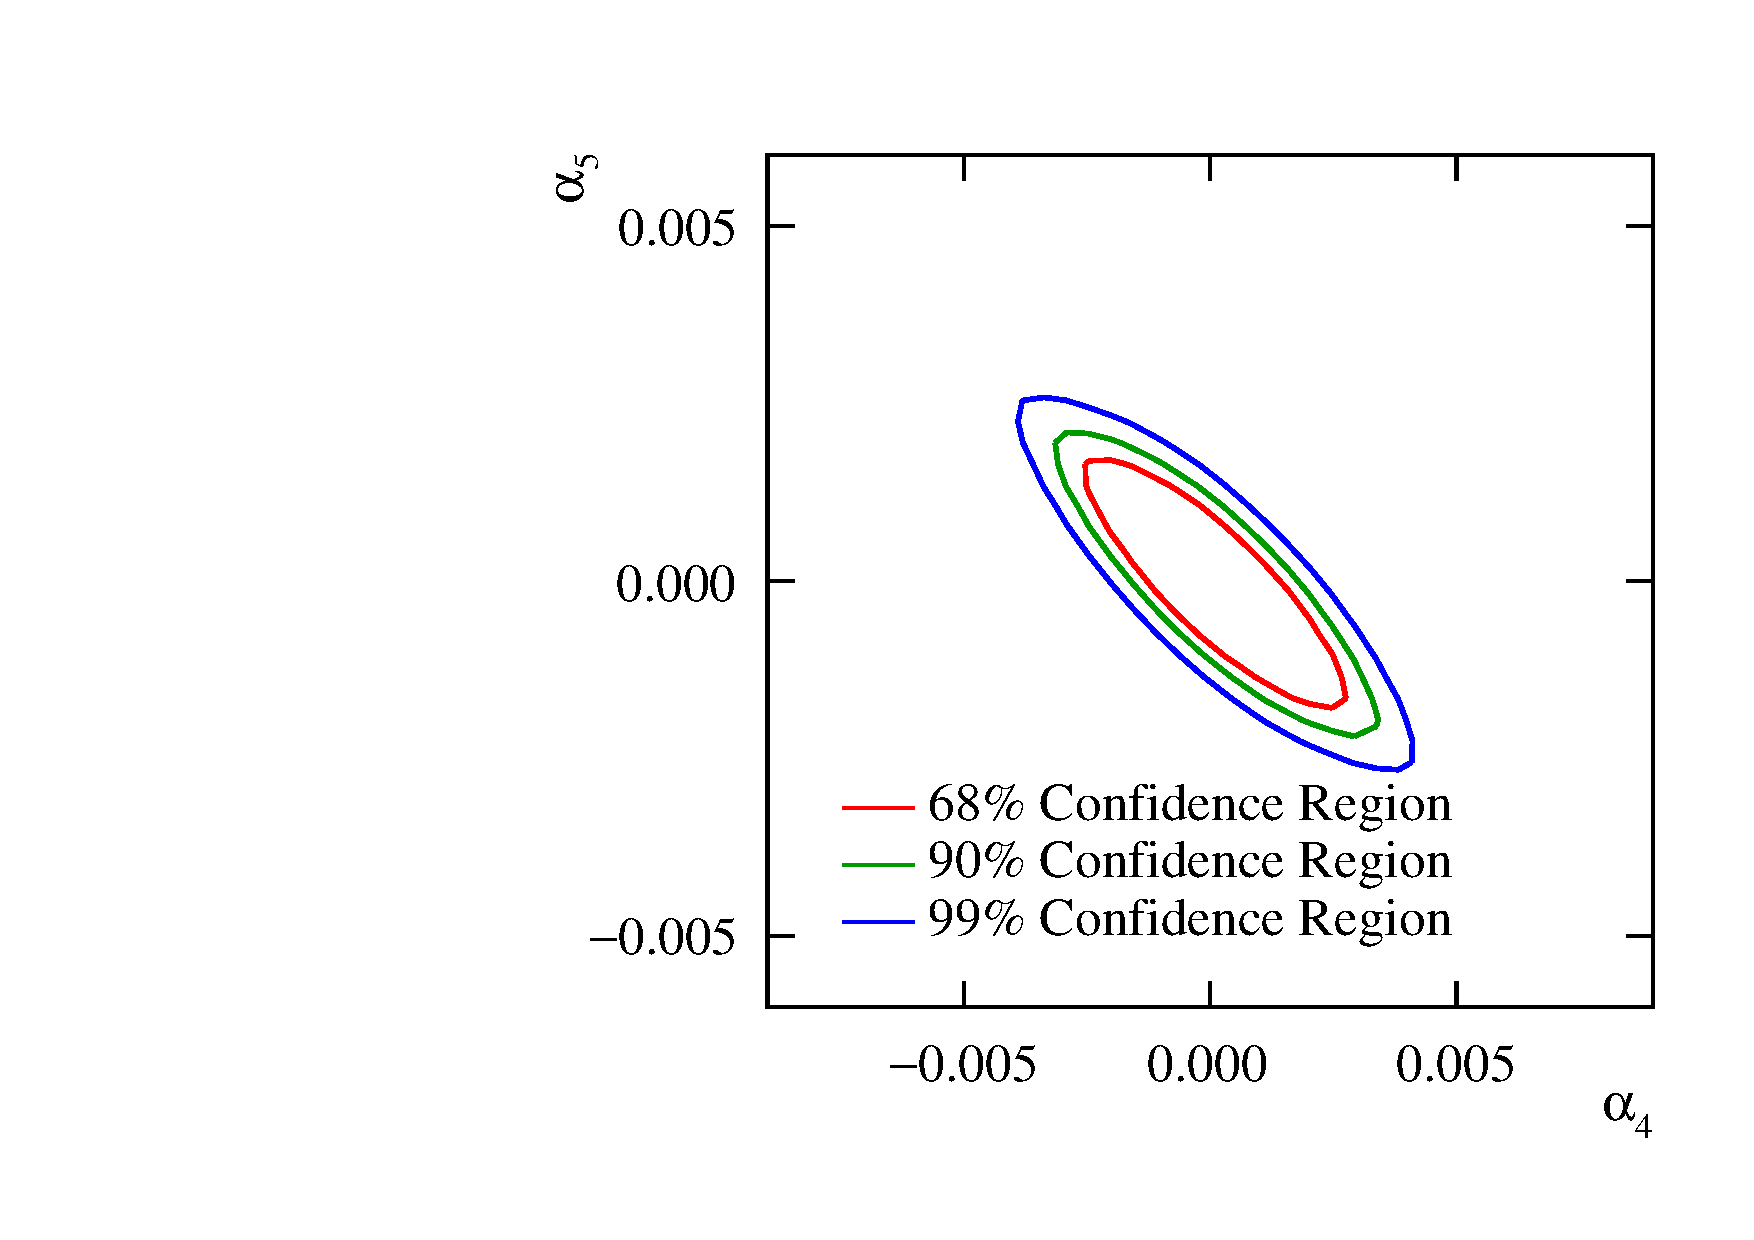
\includegraphics[width=0.5\textwidth]{PhysicsAnalysis/Plots/FinalResult/3000GeV/Final.pdf}}\hfill
\subfloat[]{\label{fig:a4finalresult3000GeV}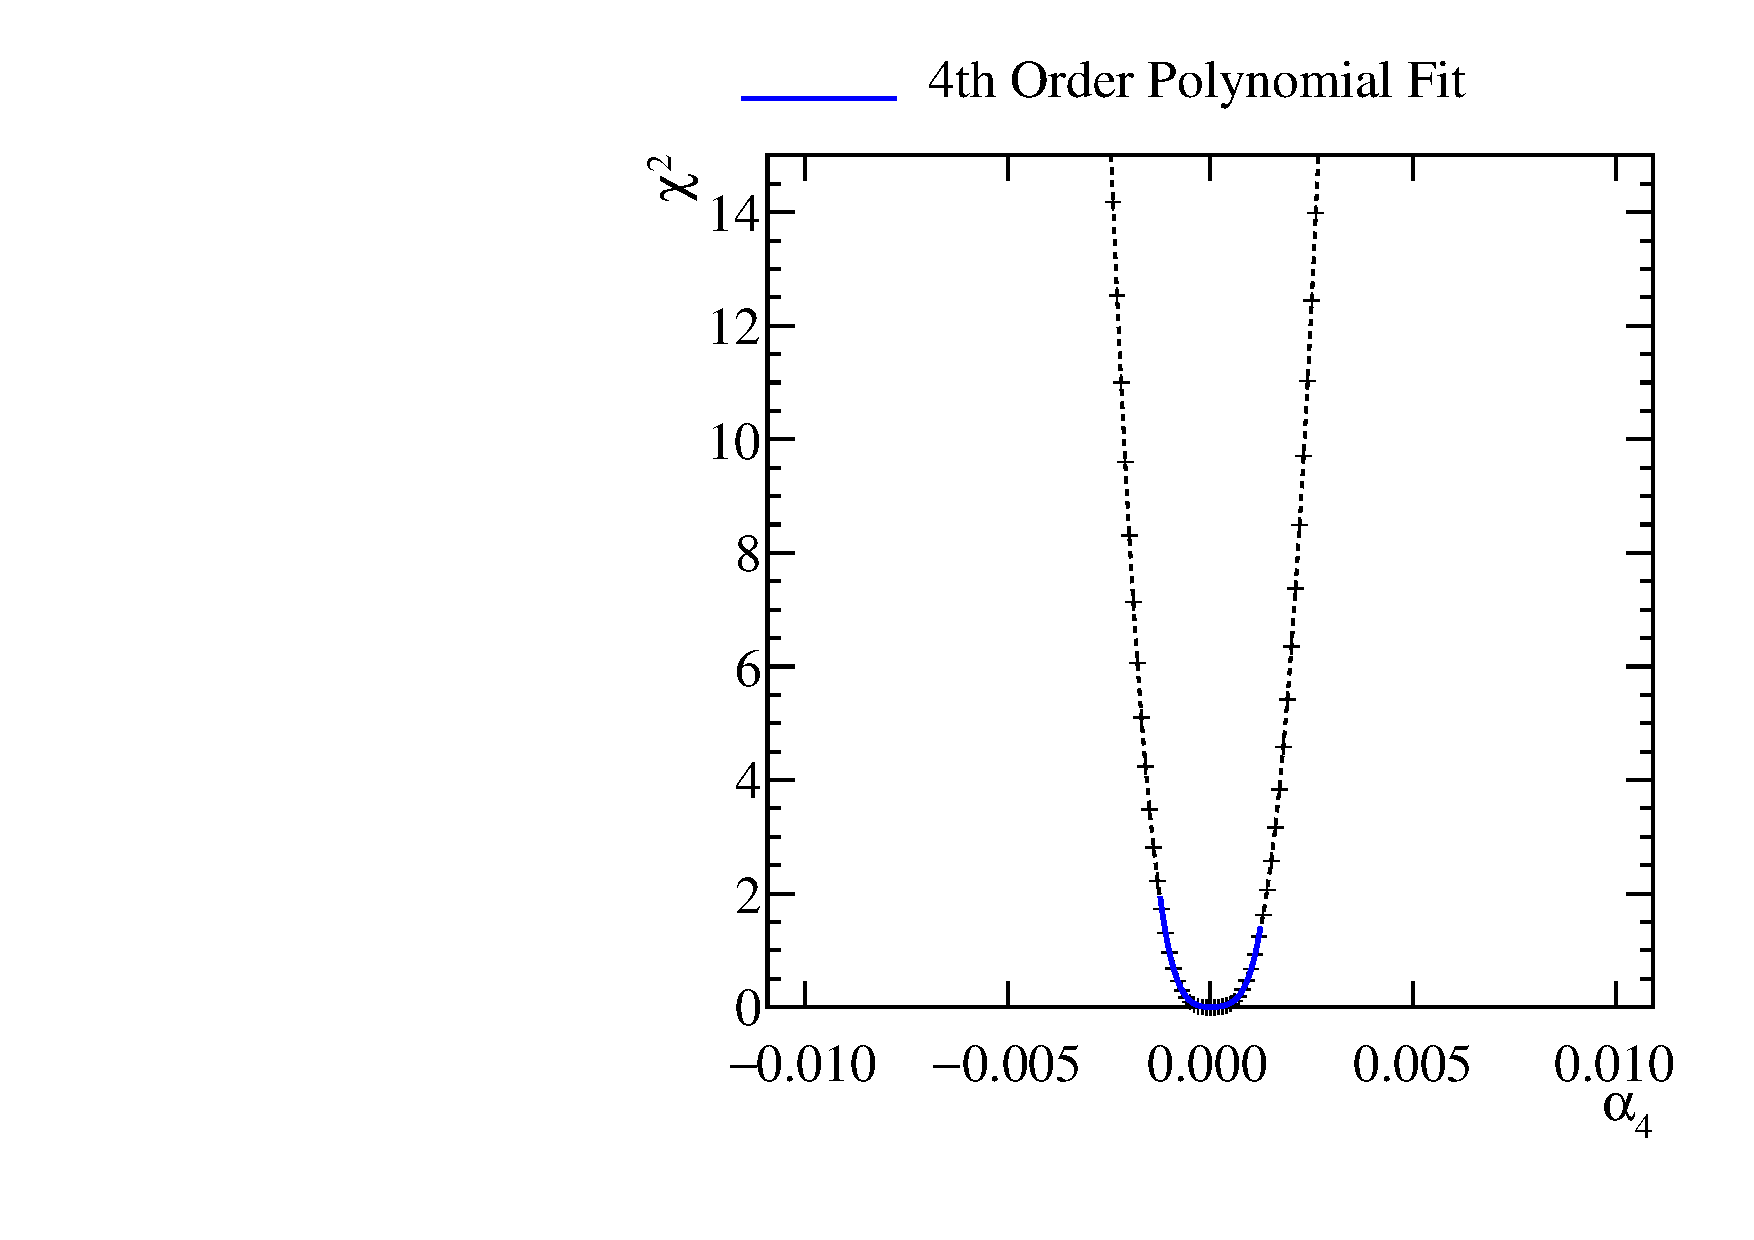
\includegraphics[width=0.5\textwidth]{PhysicsAnalysis/Plots/FinalResult/3000GeV/Final_alpha4.pdf}}
\subfloat[]{\label{fig:a5finalresult3000GeV}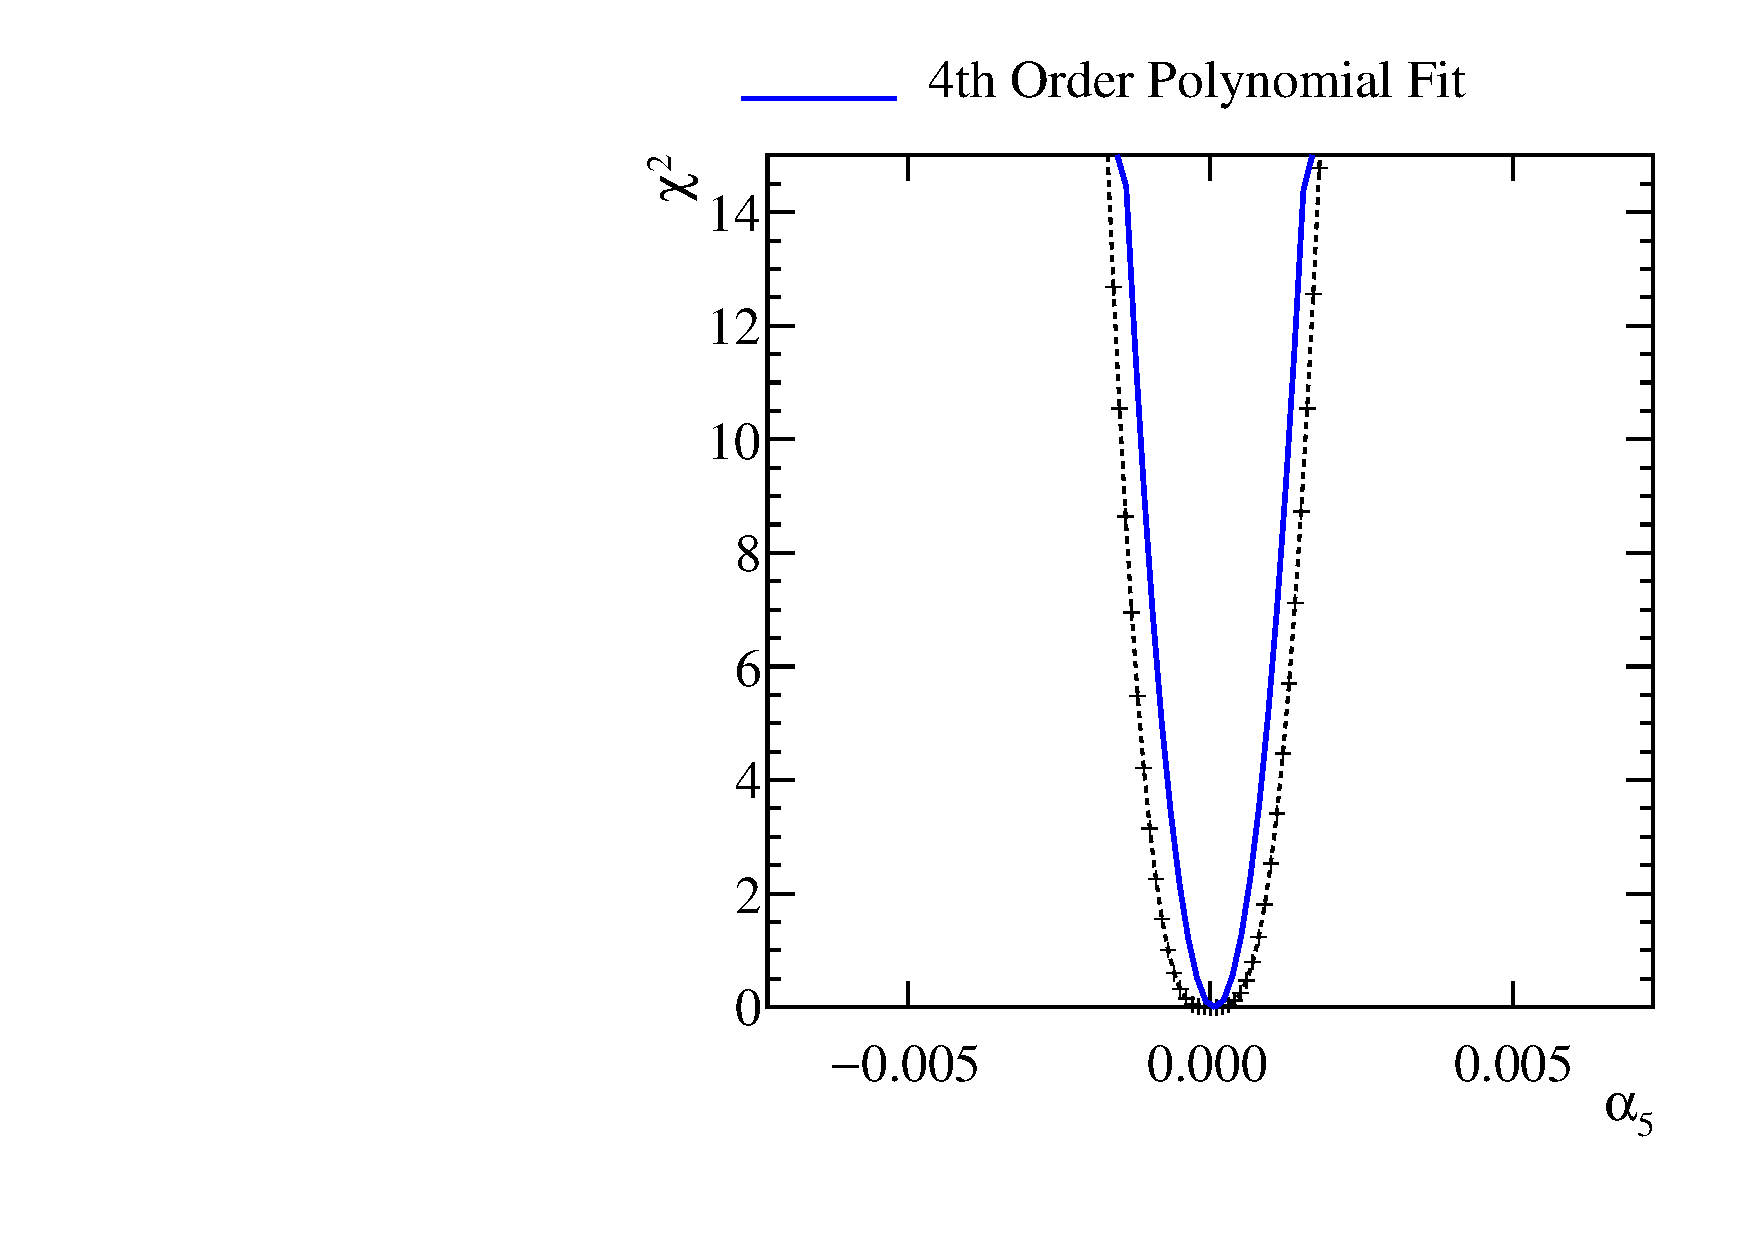
\includegraphics[width=0.5\textwidth]{PhysicsAnalysis/Plots/FinalResult/3000GeV/Final_alpha5.pdf}}
\caption[$\chi^{2}$ sensitivity distributions from a fit to $M_{VV}$ at 3~TeV.  Results include the effect of backgrounds after the application of a series of preselection cuts and MVA.  \protect\subref{fig:finalresult3000GeV} $\chi^{2}$ sensitivity contours in $\alpha_{4}$ and $\alpha_{5}$ space.  \protect\subref{fig:a4finalresult3000GeV} $\chi^{2}$ as a function of $\alpha_{4}$ assuming $\alpha_{5} = 0$.  \protect\subref{fig:a5finalresult3000GeV} $\chi^{2}$ as a function of $\alpha_{5}$ assuming $\alpha_{4} = 0$.]{$\chi^{2}$ sensitivity distributions from a fit to $M_{VV}$ at 3~TeV.  Results include the effect of backgrounds after the application of a series of preselection cuts and MVA.  \protect\subref{fig:finalresult3000GeV} $\chi^{2}$ sensitivity contours in $\alpha_{4}$ and $\alpha_{5}$ space.  \protect\subref{fig:a4finalresult3000GeV} $\chi^{2}$ as a function of $\alpha_{4}$ assuming $\alpha_{5} = 0$.  \protect\subref{fig:a5finalresult3000GeV} $\chi^{2}$ as a function of $\alpha_{5}$ assuming $\alpha_{4} = 0$.}
\label{fig:allfinalresult3000GeV}
\end{figure}

%========================================================================================
%========================================================================================
\iffalse
% Currently not including as not sure it adds much

%The sensitivity contours and the one dimensional $\chi^{2}$ distributions for $\alpha_{4}$ and $\alpha_{5}$, assuming $\alpha_{5} = 0$ and $\alpha_{4} = 0$ respectively, for the optimal jet configuration at 3~TeV using the {\nu}{\nu}qqqq signal final state are shown in figure \ref{fig:allchi2jetalgoideal3000GeV}.  Using these distributions the one sigma confidence limits on $\alpha_{4}$ is -0.000299 to 0.000300 and on $\alpha_{5}$ is -0.000178 to 0.000195.

\begin{figure}[h!]
\centering
\subfloat[]{\label{fig:chi2jetalgoideal3000GeV}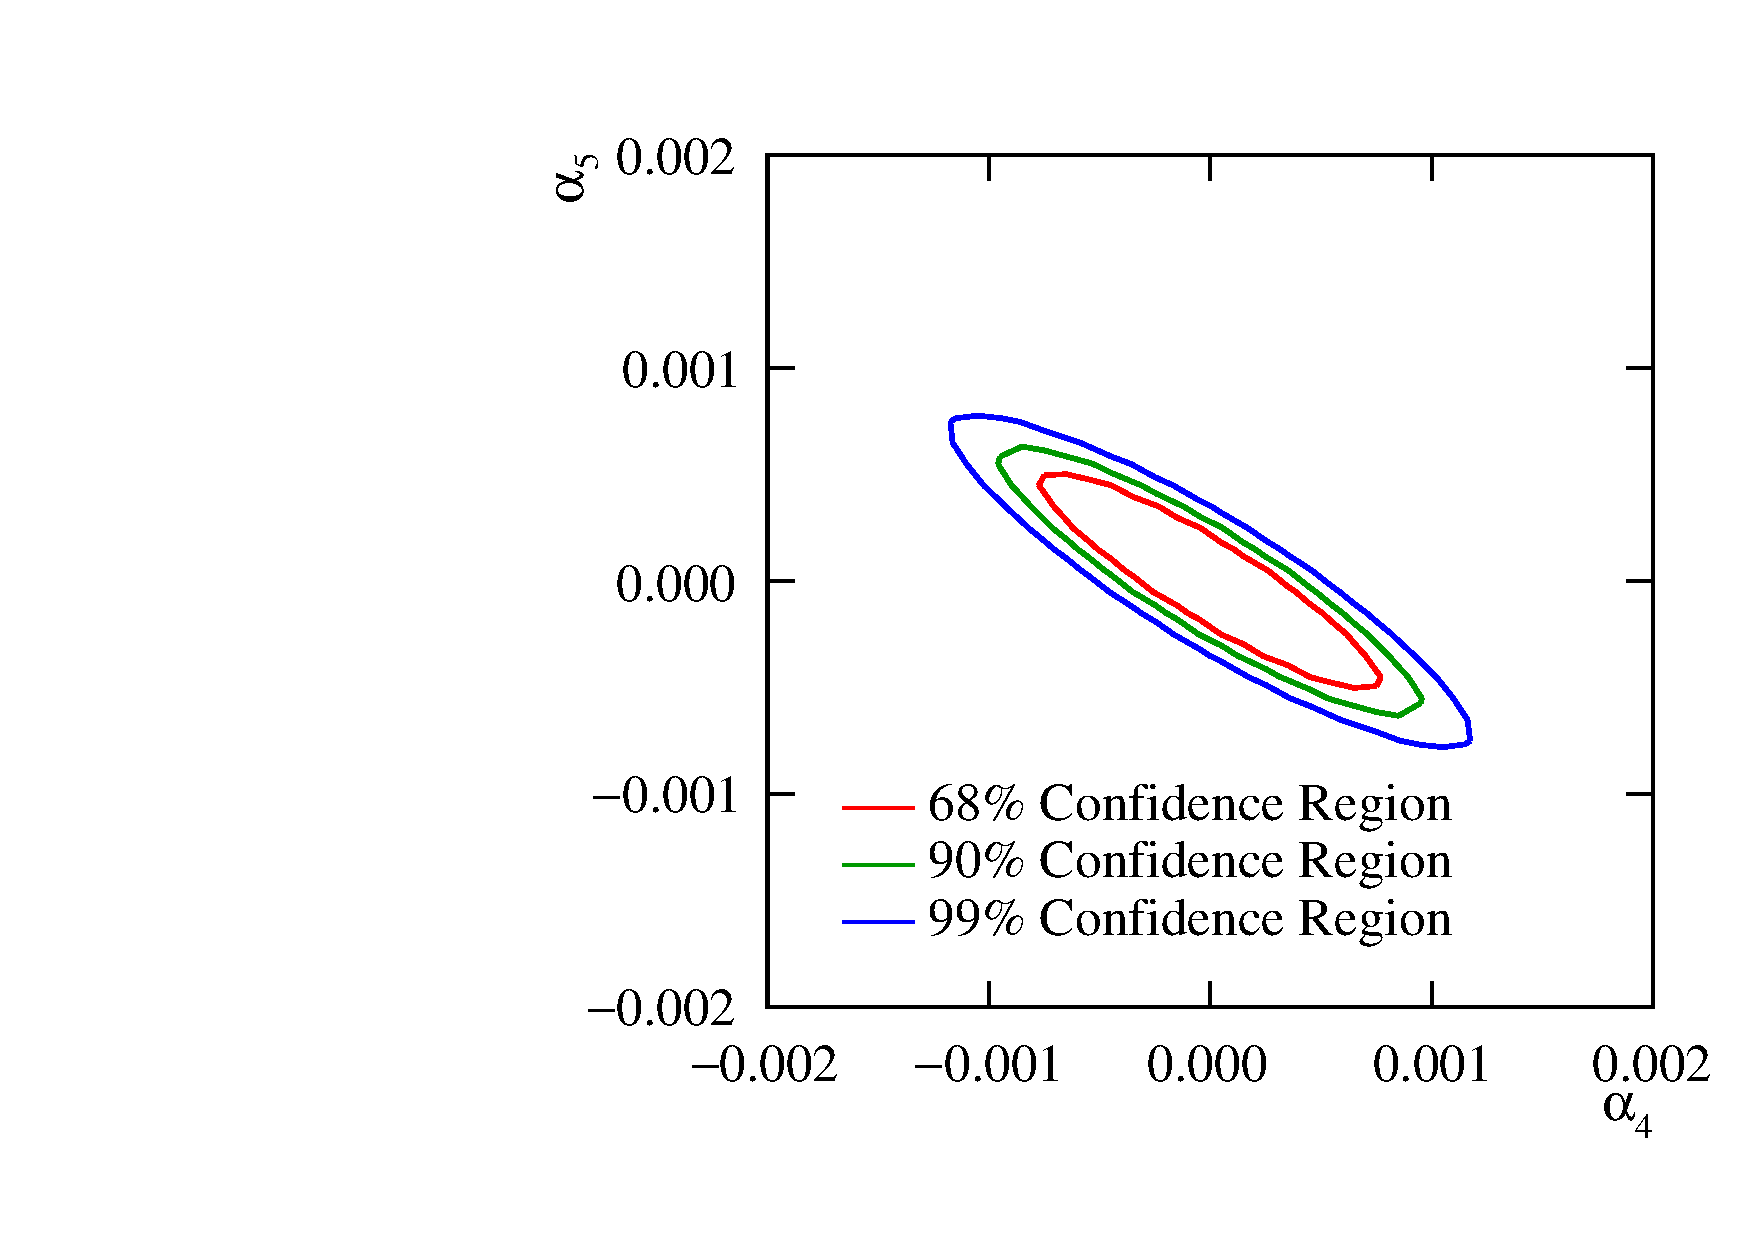
\includegraphics[width=0.5\textwidth]{PhysicsAnalysis/Plots/Chi2ContoursOptimisation/3000GeV/KtTPFOsR1p10_Optimal.pdf}}\hfill
\subfloat[]{\label{fig:a4chi2jetalgoideal3000GeV}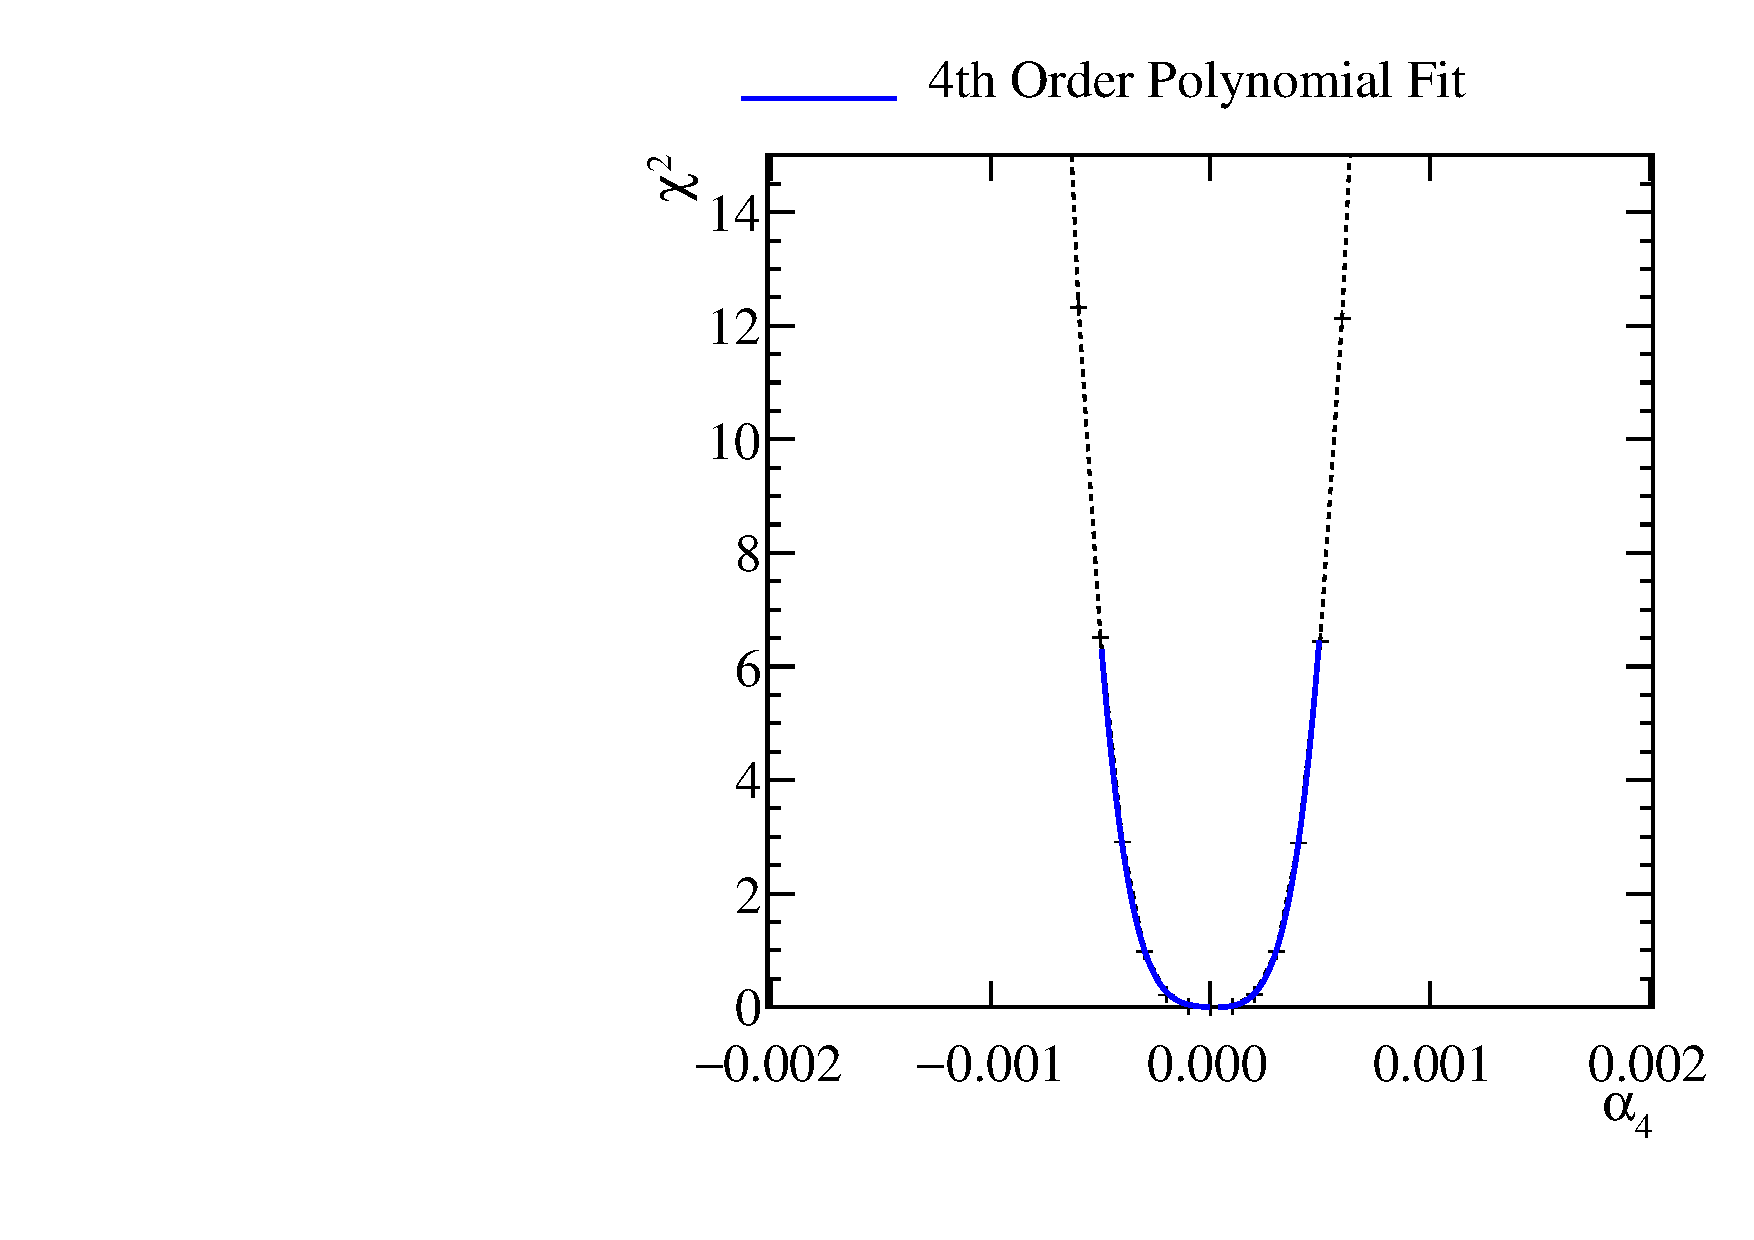
\includegraphics[width=0.5\textwidth]{PhysicsAnalysis/Plots/Chi2ContoursOptimisation/3000GeV/KtTPFOsR1p10_alpha4_Optimal.pdf}}
\subfloat[]{\label{fig:a5chi2jetalgoideal3000GeV}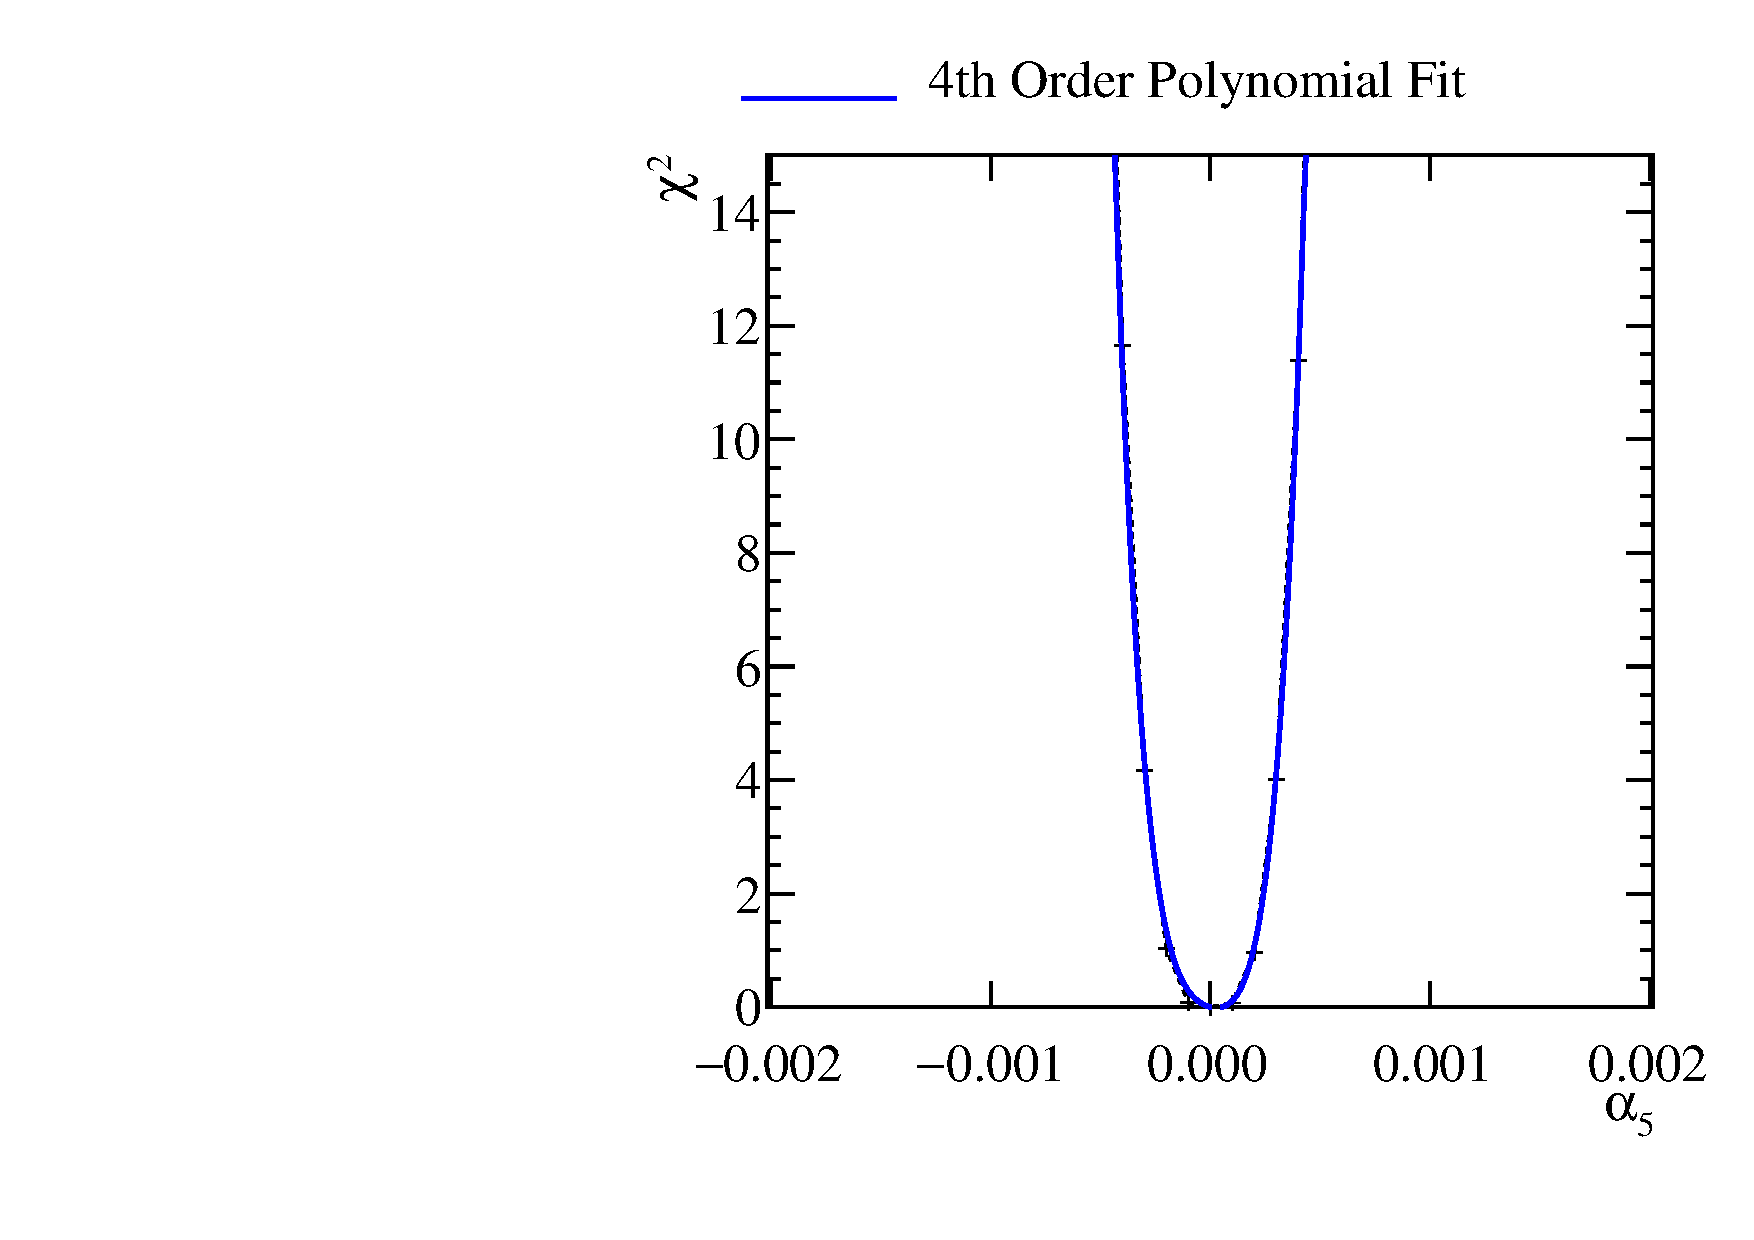
\includegraphics[width=0.5\textwidth]{PhysicsAnalysis/Plots/Chi2ContoursOptimisation/3000GeV/KtTPFOsR1p10_alpha5_Optimal.pdf}}

\caption[$\chi^{2}$ sensitivity distributions from a fit to $M_{VV}$ for the signal $\text{qqqq}\nu\nu$ final state only at 3~TeV.  These results use the optimal jet algorithm configuration of tight selected PFOs and an R parameter of 1.1 in the $k_{t}$ algorithm.  \protect\subref{fig:chi2jetalgoideal3000GeV} $\chi^{2}$ sensitivity contours in $\alpha_{4}$ and $\alpha_{5}$ space.  \protect\subref{fig:a4chi2jetalgoideal3000GeV} $\chi^{2}$ as a function of $\alpha_{4}$ assuming $\alpha_{5} = 0$.  \protect\subref{fig:a5chi2jetalgoideal3000GeV} $\chi^{2}$ as a function of $\alpha_{5}$ assuming $\alpha_{4} = 0$.]{$\chi^{2}$ sensitivity distributions from a fit to $M_{VV}$ for the signal $\text{qqqq}\nu\nu$ final state only at 3~TeV.  These results use the optimal jet algorithm configuration of tight selected PFOs and an R parameter of 1.1 in the $k_{t}$ algorithm.  \protect\subref{fig:chi2jetalgoideal3000GeV} $\chi^{2}$ sensitivity contours in $\alpha_{4}$ and $\alpha_{5}$ space.  \protect\subref{fig:a4chi2jetalgoideal3000GeV} $\chi^{2}$ as a function of $\alpha_{4}$ assuming $\alpha_{5} = 0$.  \protect\subref{fig:a5chi2jetalgoideal3000GeV} $\chi^{2}$ as a function of $\alpha_{5}$ assuming $\alpha_{4} = 0$.}
\label{fig:allchi2jetalgoideal3000GeV}
\end{figure}
\fi
%========================================================================================
%========================================================================================
